\documentclass[12pt,a4paper]{report}
\usepackage[utf8]{inputenc}
\usepackage[T1]{fontenc}
\usepackage[french]{babel}
\usepackage{geometry}
\geometry{a4paper, left=2.5cm, right=2.5cm, top=3cm, bottom=2.5cm, headheight=1.5cm}
\usepackage{eurosym}
\usepackage{amssymb}
\usepackage{graphicx}
\usepackage{hyperref}
\usepackage[table]{xcolor}
\usepackage{tabularx}
\usepackage{booktabs}
\usepackage{float}
\usepackage{fancyhdr}
\usepackage{titlesec}
\usepackage{enumitem}
\usepackage{caption}
\usepackage{longtable}
\usepackage{array}
\usepackage{setspace}
\usepackage{microtype}
\usepackage{mathptmx}
\usepackage{minitoc}
\usepackage{listings}
\lstset{
  literate={é}{{\\'e}}1 {è}{{\`e}}1 {à}{{\`a}}1 {ç}{{\c{c}}}1 {É}{{\\'E}}1 {Ê}{{\^E}}1 {Î}{{\^I}}1 {ô}{{\^o}}1 {œ}{{\oe}}1 {°}{{\textdegree}}1 {'}{{'}}1 {«}{{\guillemotleft}}1 {»}{{\guillemotright}}1
}
\usepackage{subcaption}
\usepackage{tcolorbox}
\usepackage{lastpage}
\usepackage{pdfpages}
\usepackage{tikz}
\usetikzlibrary{shapes.geometric, arrows.meta, positioning, fit, backgrounds, calc, matrix}
\newcolumntype{R}{>{\raggedright\arraybackslash}X}
\sloppy

% ── Graphics path ──
\graphicspath{{pdf_images/}{report-images/}{screenshots/}}

% ── QA Report Colors ──
\definecolor{primary}{HTML}{1e293b}
\definecolor{secondary}{HTML}{E94560}
\definecolor{success}{HTML}{2E7D32}
\definecolor{successbg}{HTML}{4CAF50}
\definecolor{warning}{HTML}{F57C00}
\definecolor{warningbg}{HTML}{F59E0B}
\definecolor{danger}{HTML}{D32F2F}
\definecolor{dangerbg}{HTML}{DC2626}
\definecolor{codebg}{HTML}{1E1E2E}
\definecolor{codefg}{HTML}{CDD6F4}
\definecolor{linkblue}{HTML}{1565C0}
\definecolor{expectedbg}{HTML}{E6F9ED}
\definecolor{actualbg}{HTML}{FEF2F2}
\definecolor{expectedhdr}{HTML}{238636}

% ── Dashboard Diagram Colors ──
\definecolor{accent}{HTML}{0d9668}
\definecolor{blueC}{HTML}{2563eb}
\definecolor{purpleC}{HTML}{7c3aed}
\definecolor{orangeC}{HTML}{ea580c}
\definecolor{pinkC}{HTML}{db2777}
\definecolor{greenC}{HTML}{16a34a}
\definecolor{grayC}{HTML}{64748b}
\definecolor{graylight}{HTML}{f1f5f9}
\definecolor{bgcode}{HTML}{f8fafc}
\definecolor{yellowC}{HTML}{ca8a04}

% ── TikZ Styles ──
\tikzset{
    ndGreen/.style={rectangle, rounded corners=4pt, draw=accent, fill=accent!8, minimum width=3.5cm, minimum height=1cm, align=center, font=\footnotesize, text=primary, line width=0.8pt},
    ndBlue/.style={rectangle, rounded corners=4pt, draw=blueC, fill=blueC!8, minimum width=3.5cm, minimum height=1cm, align=center, font=\footnotesize, text=primary, line width=0.8pt},
    ndPurple/.style={rectangle, rounded corners=4pt, draw=purpleC, fill=purpleC!8, minimum width=3.5cm, minimum height=1cm, align=center, font=\footnotesize, text=primary, line width=0.8pt},
    ndOrange/.style={rectangle, rounded corners=4pt, draw=orangeC, fill=orangeC!8, minimum width=3.5cm, minimum height=1cm, align=center, font=\footnotesize, text=primary, line width=0.8pt},
    ndPink/.style={rectangle, rounded corners=4pt, draw=pinkC, fill=pinkC!8, minimum width=3.5cm, minimum height=1cm, align=center, font=\footnotesize, text=primary, line width=0.8pt},
    ndGreenC/.style={rectangle, rounded corners=4pt, draw=greenC, fill=greenC!8, minimum width=3.5cm, minimum height=1cm, align=center, font=\footnotesize, text=primary, line width=0.8pt},
    ndGray/.style={rectangle, rounded corners=4pt, draw=grayC, fill=grayC!8, minimum width=3.5cm, minimum height=1cm, align=center, font=\footnotesize, text=primary, line width=0.8pt},
    ndGrayS/.style={rectangle, rounded corners=4pt, draw=grayC, fill=grayC!8, minimum width=2.2cm, minimum height=0.9cm, align=center, font=\footnotesize, text=primary, line width=0.8pt},
    ndYellow/.style={rectangle, rounded corners=4pt, draw=yellowC, fill=yellowC!8, minimum width=3.5cm, minimum height=1cm, align=center, font=\footnotesize, text=primary, line width=0.8pt},
    bxGreen/.style={rectangle, rounded corners=6pt, draw=accent, fill=accent!4, inner sep=10pt, line width=1.2pt},
    bxBlue/.style={rectangle, rounded corners=6pt, draw=blueC, fill=blueC!4, inner sep=10pt, line width=1.2pt},
    bxPurple/.style={rectangle, rounded corners=6pt, draw=purpleC, fill=purpleC!4, inner sep=10pt, line width=1.2pt},
    bxOrange/.style={rectangle, rounded corners=6pt, draw=orangeC, fill=orangeC!4, inner sep=10pt, line width=1.2pt},
    bxPink/.style={rectangle, rounded corners=6pt, draw=pinkC, fill=pinkC!4, inner sep=10pt, line width=1.2pt},
    bxGreenC/.style={rectangle, rounded corners=6pt, draw=greenC, fill=greenC!4, inner sep=10pt, line width=1.2pt},
    bxGray/.style={rectangle, rounded corners=6pt, draw=grayC, fill=grayC!4, inner sep=10pt, line width=1.2pt},
    bxYellow/.style={rectangle, rounded corners=6pt, draw=yellowC, fill=yellowC!4, inner sep=10pt, line width=1.2pt},
    lG/.style={font=\small\bfseries, text=accent},
    lB/.style={font=\small\bfseries, text=blueC},
    lP/.style={font=\small\bfseries, text=purpleC},
    lO/.style={font=\small\bfseries, text=orangeC},
    lPk/.style={font=\small\bfseries, text=pinkC},
    lGC/.style={font=\small\bfseries, text=greenC},
    lGr/.style={font=\small\bfseries, text=grayC},
    lY/.style={font=\small\bfseries, text=yellowC},
    arw/.style={-{Stealth[length=5pt]}, line width=0.8pt, color=primary},
    lbl/.style={font=\tiny, text=primary, fill=white, inner sep=1pt},
    darw/.style={-{Stealth[length=5pt]}, dashed, line width=0.8pt, color=primary},
    ucG/.style={ellipse, draw=accent, fill=accent!8, minimum width=3.2cm, minimum height=0.7cm, align=center, font=\tiny, text=primary, line width=0.6pt},
    ucB/.style={ellipse, draw=blueC, fill=blueC!8, minimum width=3.2cm, minimum height=0.7cm, align=center, font=\tiny, text=primary, line width=0.6pt},
    actG/.style={circle, draw=accent, fill=accent!10, minimum size=0.9cm, font=\tiny\bfseries, text=primary, line width=0.8pt, align=center},
    actB/.style={circle, draw=blueC, fill=blueC!10, minimum size=0.9cm, font=\tiny\bfseries, text=primary, line width=0.8pt, align=center},
    actP/.style={circle, draw=purpleC, fill=purpleC!10, minimum size=0.9cm, font=\tiny\bfseries, text=primary, line width=0.8pt, align=center},
    cls/.style={rectangle, rounded corners=2pt, draw=blueC, fill=blueC!5, text width=5cm, align=left, font=\tiny, line width=0.8pt},
    spG/.style={rectangle, rounded corners=3pt, draw=accent, fill=accent!10, minimum width=2cm, minimum height=0.6cm, font=\tiny\bfseries, text=primary, line width=0.8pt, align=center},
    spB/.style={rectangle, rounded corners=3pt, draw=blueC, fill=blueC!10, minimum width=2cm, minimum height=0.6cm, font=\tiny\bfseries, text=primary, line width=0.8pt, align=center},
    spP/.style={rectangle, rounded corners=3pt, draw=purpleC, fill=purpleC!10, minimum width=2cm, minimum height=0.6cm, font=\tiny\bfseries, text=primary, line width=0.8pt, align=center},
    spO/.style={rectangle, rounded corners=3pt, draw=orangeC, fill=orangeC!10, minimum width=2cm, minimum height=0.6cm, font=\tiny\bfseries, text=primary, line width=0.8pt, align=center},
    spGr/.style={rectangle, rounded corners=3pt, draw=grayC, fill=grayC!10, minimum width=2cm, minimum height=0.6cm, font=\tiny\bfseries, text=primary, line width=0.8pt, align=center},
    snote/.style={rectangle, rounded corners=2pt, draw=grayC!40, fill=graylight, font=\tiny\bfseries, text=primary, align=center, inner sep=3pt},
}

% ── Code listings ──
\lstset{
    backgroundcolor=\color{codebg},
    basicstyle=\ttfamily\small\color{codefg},
    breaklines=true,
    frame=single,
    rulecolor=\color{gray!30},
    showstringspaces=false
}

% ── QA Report macros ──
\newcommand{\twoimages}[4]{%
\begin{figure}[H]
    \centering
    \begin{subfigure}[b]{0.48\textwidth}
        \includegraphics[width=\textwidth]{#1}
        \caption{#2}
    \end{subfigure}
    \hfill
    \begin{subfigure}[b]{0.48\textwidth}
        \includegraphics[width=\textwidth]{#3}
        \caption{#4}
    \end{subfigure}
\end{figure}
}

\newcommand{\bugtable}[2]{%
\begin{center}
\begin{tabular}{|p{0.47\textwidth}|p{0.47\textwidth}|}
\hline
\cellcolor{expectedhdr}\textcolor{white}{\textbf{Expected}} & \cellcolor{dangerbg}\textcolor{white}{\textbf{Obtained}} \\
\hline
\cellcolor{expectedbg} #1 & \cellcolor{actualbg} #2 \\
\hline
\end{tabular}
\end{center}
}

% ── Colors ──
\definecolor{chaptercolor}{HTML}{1B75BC}
\definecolor{sectioncolor}{HTML}{1B75BC}
\definecolor{captioncolor}{HTML}{1B75BC}
\definecolor{linkcolor}{HTML}{1B75BC}
\definecolor{rulecolor}{HTML}{C0C0C0}

% ── Hyperref ──
\hypersetup{colorlinks=true, linkcolor=linkcolor, urlcolor=linkcolor, citecolor=linkcolor}

% ── Setup Marks for Chapter ──
\makeatletter
\renewcommand{\chaptermark}[1]{\markboth{Chapitre \thechapter. #1}{}}
\makeatother

% ── Headers/Footers ──
\pagestyle{fancy}
\fancyhf{}
\fancyhead[C]{\textbf{\leftmark}}
\fancyfoot[L]{\textbf{HPS}}
\fancyfoot[C]{\textbf{\thepage}}
\fancyfoot[R]{\textbf{Année universitaire 2025--2026}}
\renewcommand{\headrulewidth}{1pt}
\renewcommand{\footrulewidth}{1pt}

% Redéfinir le style 'plain' (utilisé par défaut sur les pages de chapitres) pour avoir le même header/footer
\fancypagestyle{plain}{
  \fancyhf{}
  \fancyhead[C]{\textbf{\leftmark}}
  \fancyfoot[L]{\textbf{HPS}}
  \fancyfoot[C]{\textbf{\thepage}}
  \fancyfoot[R]{\textbf{Année universitaire 2025--2026}}
  \renewcommand{\headrulewidth}{1pt}
  \renewcommand{\footrulewidth}{1pt}
}

% ── Chapter/Section styling ──
\definecolor{mygreen}{HTML}{1A8438}
\titleformat{\chapter}[display]
  {\vspace*{\fill}\centering\color{black}\Huge\bfseries}
  {\textcolor{mygreen}{\rule{\textwidth}{1.5pt}}\vspace{10pt}\\ \textbf{Chapitre \thechapter\ :}}
  {10pt}
  {\Huge}[\vspace{10pt}\textcolor{mygreen}{\rule{\textwidth}{1.5pt}}\vspace*{\fill}\newpage]

\titleformat{name=\chapter,numberless}[display]
  {\normalfont\Huge\bfseries\centering}
  {}
  {0pt}
  {\Huge}

\titlespacing*{\chapter}{0pt}{0pt}{0pt}

\titleformat{\section}
  {\fontsize{18}{22}\bfseries\color{sectioncolor}\raggedright}
  {\thesection}{1em}{}
\titleformat{\subsection}
  {\normalsize\bfseries\color{sectioncolor}\raggedright}
  {\thesubsection}{1em}{}
\titleformat{\subsubsection}
  {\normalsize\color{sectioncolor}\raggedright}
  {\thesubsubsection}{1em}{}

% ── Caption styling ──
\captionsetup{labelsep=colon, labelfont={bf,color=captioncolor}, textfont={color=captioncolor}, justification=centering}

% ── Custom frontmatter commands ──
\newcommand{\frontmattertitle}[1]{%
  \vspace*{1cm}
  \begin{center}
    \fontsize{24}{28}\bfseries\selectfont #1
  \end{center}
  \vspace{1.5cm}
}

% ── Custom chapter header bar ──
\newcommand{\chapterbar}[1]{%
  \noindent\makebox[\textwidth]{\textcolor{rulecolor}{\rule{\textwidth}{1pt}}}\\[2pt]
  \centering{\color{chaptercolor}\fontsize{18}{22}\bfseries\selectfont #1}\\[2pt]
  \noindent\makebox[\textwidth]{\textcolor{rulecolor}{\rule{\textwidth}{1pt}}}
  \vspace{10pt}
}

% ── Reduce spacing ──
\setlength{\parindent}{0pt}
\setlength{\parskip}{6pt}

\setstretch{1.5}

% ══════════════════════════════════════════════════════════════════
% DOCUMENT
% ══════════════════════════════════════════════════════════════════
\begin{document}
\pagenumbering{arabic}
\dominitoc
\nomtcrule

% ── Frontmatter: Cover, Dédicace, Remerciements, Abstract, Résumé, Glossaire, ToC ──
% ══════════════════════════════════════════════════════════════════
% COVER PAGE
% ══════════════════════════════════════════════════════════════════
% --- Page Réseaux ou autre PDF

\includepdf{IIR.pdf}

% ══════════════════════════════════════════════════════════════════
% DÉDICACE
% ══════════════════════════════════════════════════════════════════
\newpage
\chapter*{Dédicace}
\addcontentsline{toc}{chapter}{Dédicace}

\begin{center}
\fontsize{16}{19}\itshape\selectfont
À mes chers parents,\\
pour tous leurs sacrifices, leur amour, leur tendresse, leur soutien et leurs prières tout au long de mes études.\\
À ma chère famille, pour leur encouragement permanent.\\
À mes professeurs et amis, pour leur aide et leur soutien.\\
Je vous dédie ce travail.
\end{center}

% ══════════════════════════════════════════════════════════════════
% REMERCIEMENTS
% ══════════════════════════════════════════════════════════════════
\newpage
\chapter*{Remerciements}
\addcontentsline{toc}{chapter}{Remerciements}

\begin{center}
\fontsize{16}{19}\itshape\selectfont
Je tiens tout d'abord à remercier Madame Salima MISSOUR, mon encadrante de stage pour son suivi et son accompagnement tout au long de ce stage, ainsi que Madame Meryem Fouzair de m'avoir accueilli dans le premier jour de mon stage.\\[10pt]

Mes remerciements vont également à Monsieur Fabrice Soto et Jérôme PEIGNIEN, pour leurs encadrements techniques qui m'a permis de monter en compétences sur différents sujets et pour leurs présences et leurs disponibilités.\\[10pt]

Je tiens également à exprimer ma gratitude à l'ensemble de l'équipe de tests, de m'avoir accueilli, accompagné et pris de temps de répondre à mes questions.\\[10pt]

Je tiens également à exprimer ma reconnaissance à Mr. Ali IDMANSOUR pour avoir supervisé mon stage, pour ses remarques et ses conseils. Mes remerciements vont aussi à l'ensemble du corps professoral de l'université EMSI pour leurs efforts afin de réussir cette année exceptionnelle.\\[10pt]

Enfin, un chaleureux remerciement à ma famille, particulièrement, mes parents qui m'ont apporté, sans réserve, tout le soutien et l'affection nécessaires pour le bon déroulement de mon stage.
\end{center}

% ══════════════════════════════════════════════════════════════════
% RÉSUMÉ
% ══════════════════════════════════════════════════════════════════
\newpage
\chapter*{Résumé}
\addcontentsline{toc}{chapter}{Résumé}

{\fontsize{14}{17}\selectfont
Ce présent document résume tous les travaux effectués pendant mon stage PFE, qui s'intitule « Automatisation des tests », au titre du projet de fin d'études.

L'automatisation des tests est un moyen qui est de plus en plus apprécié par les organisations. Elle se présente comme une solution efficace permettant d'éviter les erreurs humaines lors de la répétition d'exécution des tests et gagner du temps. D'où l'idée d'intégrer une équipe d'automatisation de test du groupe HPS qui compte parmi les grands éditeurs de logiciel monétique. Ma mission durant ce stage est l'automatisation des tests de quelques fonctionnalités de la solution monétique d'HPS.

Pour aboutir à mes fins et accomplir ma mission, il a été indispensable de suivre un ensemble d'étapes : en commençant par les formations puis définition de l'environnement de test, l'analyse des cahiers de spécification technique, la conception des tests et des jeux de données, l'implémentation des scénarios de test, l'exécution manuellement des tests avant de les automatisés et enfin la rédaction du rapport au fur et à mesure de la réalisation de la mission.

Au-delà de l'automatisation classique, ce projet introduit une approche innovante : le développement d'un \textbf{QA Cypress Generator Dashboard}, une plateforme full-stack alimentée par l'\textbf{IA (Mistral)} et l'\textbf{orchestration de workflows (n8n)}, permettant aux testeurs QA de générer, exécuter et surveiller des scripts de tests Cypress E2E sans écrire une seule ligne de code.

\vspace{10pt}
\textbf{Mots clés :} Automatisation des tests, Cypress, React, Node.js, PowerCARD, Assurance Qualité, IA, n8n, Microservices
}

% ══════════════════════════════════════════════════════════════════
% GLOSSAIRE
% ══════════════════════════════════════════════════════════════════
\newpage
\chapter*{Glossaire}
\addcontentsline{toc}{chapter}{Glossaire}

{\fontsize{14}{17}\selectfont
\begin{description}[leftmargin=3cm,style=nextline]
\item[AI] Artificial Intelligence (Intelligence Artificielle)
\item[API] Application Programming Interface
\item[ATM] Automated Teller Machine
\item[BRD] Business Requirement Description
\item[BSD] Business Solution Description
\item[DB] Data Base
\item[E2E] End-To-End (Test de bout en bout)
\item[EMSI] Ecole Marocaine des Sciences de l'Ingénieur
\item[FTP] File Transfer Protocole
\item[FTPS] File Transfer Protocole Secure
\item[HPS] Hightech Payment Systems
\item[HSBC] Hong-Kong and Shanghai Banking Corporation
\item[ISTQB] International Software Testing Qualifications Board
\item[JEE] Java Entreprise Edition
\item[JSF] Java Server Faces
\item[JWT] JSON Web Token
\item[LLM] Large Language Model
\item[MCP] Model Context Protocol
\item[n8n] Outil d'automatisation de workflows open-source
\item[PTT] PowerTools Tests
\item[PWC] PowerCARD
\item[QA] Quality Assurance (Assurance Qualité)
\item[REST] Representational State Transfer
\item[SFTP] SSH File Transfer Protocol
\item[SPA] Single Page Application
\item[SQL] Structured Query Language
\item[SSE] Server-Sent Events
\item[UI] User Interface
\item[UNIX] Unix
\item[WS] Web Service
\item[XML] Extensible Markup Language
\end{description}
}

% ══════════════════════════════════════════════════════════════════
% TABLE DES MATIÈRES
% ══════════════════════════════════════════════════════════════════
\newpage
\tableofcontents

% ══════════════════════════════════════════════════════════════════
% LISTE DES FIGURES ET TABLEAUX
% ══════════════════════════════════════════════════════════════════
\newpage
\listoffigures
\newpage
\listoftables


% ── Introduction Générale ──
% ══════════════════════════════════════════════════════════════════
% INTRODUCTION GÉNÉRALE
% ══════════════════════════════════════════════════════════════════
\newpage
\pagenumbering{arabic}
\setcounter{page}{1}
\chapter*{Introduction Générale}
\addcontentsline{toc}{chapter}{Introduction Générale}

L'informatique a bel et bien révolutionné le monde actuel où nous vivons, particulièrement à partir des années quatre-vingt-dix. Elle est présente partout : dans le travail, les communications, les transports, le commerce, les services, etc. On est devenu presque dépendant de cet outil qui a pratiquement envahit notre existence. Certes, l'informatique a beaucoup contribué à l'amélioration des conditions de notre vie. Elle nous a permis d'exécuter rapidement et efficacement des tâches, autrefois très lentes et compliquées. C'est pourquoi, elle est intégrée dans quasiment tous les secteurs d'activité : l'administration, l'industrie, le commerce, la finance, etc.

Dans le cadre de ma formation à l'université EMSI en génie Informatique, j'ai effectué un stage de fin d'études de 6 mois chez HPS.

HPS est un leader mondialement reconnu dans l'édition de solutions de paiement électronique dédiées aux institutions financières, elle fournit des solutions et des services à haute valeur ajoutée autour de sa suite de solutions de paiement électronique PowerCARD.

Ce stage a pour but de valider mes compétences et savoir acquis durant ma formation en accompagnant l'équipe de test d'HPS dans leurs activités de test, d'automatisation de test.

Cette expérience m'a permis de mettre en pratique tout ce que j'ai appris durant ma formation et aussi d'avoir une vision globale sur les activités de l'équipe de test de HPS.

Le rapport présente en premier lieu l'entreprise, le service d'accueil et l'équipe avec laquelle j'ai travaillé, puis le contexte global des missions réalisées ainsi que les détails de chacune d'elle en expliquant le contexte, problématique, la méthodologie utilisée et les résultats obtenus pour enfin finir avec une conclusion.


% ── Chapitre I: Présentation de l'organisme d'accueil ──
% ══════════════════════════════════════════════════════════════════
% CHAPITRE I — Présentation de l'organisme d'accueil
% ══════════════════════════════════════════════════════════════════
\newpage
\setcounter{chapter}{0}
\chapter{Présentation de l'organisme d'accueil}
\vspace{1cm}
\minitoc
\newpage

\textbf{Introduction}

Dans le cadre de l'industrie financière mondiale, le traitement sécurisé et efficace des transactions est d'une importance capitale. HPS Group s'inscrit dans ce contexte en tant qu'acteur majeur fournissant des solutions de paiement électronique de pointe. Ce chapitre a pour objectif de présenter la société d'accueil, HPS, ainsi que sa filiale ACPQUALIFE. Nous examinerons la structure organisationnelle, les secteurs d'activité, et les valeurs fondamentales de l'entreprise, afin de comprendre l'environnement professionnel dans lequel s'est déroulé ce stage de fin d'études et les exigences de qualité rigoureuses qui y sont appliquées.
\vspace{10pt}

\section{HPS Group}

HPS (Hightech Payment Systems) est un groupe compté parmi les leaders mondiaux dans l'édition et le développement des solutions de paiements électroniques, qui sont dédiées aux institutions financières. Son siège se trouve à Nearshore Park de Casablanca au Maroc HPS fournit des solutions progicielles basées sur la famille de produits PowerCARD, ainsi que les différents services associés, tels que l'implémentation du système et sa maintenance. Elle conçoit et fournit des solutions complètes, modulaires et intégrées. Grâce à PowerCARD, hautement paramétrable, HPS traite tous les types de cartes (cartes de crédit, cartes de débit, cartes prépayées, cartes de fidélité, cartes d'entreprises, ...), via tous les canaux (GAB, TPE, internet et mobile, ...) et pour toutes les catégories de commerçants (banques, sociétés, compagnies, opérateurs, ...)

\section{Historique d'HPS}

Fondée en 1995 par un groupe de consultants et d'experts, HPS est un fournisseur de solution monétique permettant la gestion du paiement électronique multi canal prenant en charge le terminal de paiement électronique, le guichet automatique bancaire, Internet et le mobile. Elle est certifiée par les principaux organismes internationaux tels que Visa, MasterCard, Diners Club, JCB et American Express.

HPS a progressivement étendu sa présence géographique en créant HPS Dubaï en 2003, puis HPS Europe en 2008. L'objectif premier de ces deux bureaux était de développer l'activité commerciale dans ces régions en délocalisant une force de vente dédiée, chargée de la commercialisation en direct et de l'animation d'un réseau de partenaires régionaux. En 2017, deux nouveaux bureaux sont ouverts à Singapore et Lausanne.

\section{Secteur d'activité}

Le progiciel PowerCARD offert par HPS est une solution de paiement électronique évoluée et hautement sécurisée. Il toute la chaîne de valeur du paiement et offre aux clients une panoplie de solutions à forte valeur ajoutée pour piloter et gérer leurs risques :

\begin{itemize}[leftmargin=*]
\item \textbf{PowerCARD-eSecure} : étape supplémentaire pour les paiements en ligne afin de lier une autorisation financière avec une authentification en ligne (ACS - 3D Secure).
\item \textbf{PowerCARD-ACH} : solution pour la gestion des autorisations et compensation entre différentes chambres.
\item \textbf{PowerCARD-Issuer} : services complets pour l'émission et la gestion de toutes les cartes sous tous les formats.
\item \textbf{PowerCARD-ATM} : solution self-service globale qui permet aux institutions financières et aux détaillants une gestion et une optimisation des GAB.
\item \textbf{PowerCARD-xPOS} : système de gestion des demandes d'autorisation et de gestion des transactions pour tout type de terminal de paiement électronique.
\item \textbf{PowerCARD-Tokenisation} : solution complète qui supporte l'émission, le provisionnement et le stockage de jetons de la part d'un demandeur de jeton.
\item \textbf{PowerCARD-Fraud} : solution de gestion de fraude autonome, qui contrôle en temps réel ou différé les autorisations venant d'un quelconque système.
\item \textbf{PowerCARD-eCommerce} : solution multi-commerçants et multi-acquéreurs pour une gestion de paiement e-commerce.
\item \textbf{PowerCARD-Switch} : routing, stand-in et autorisation dans un environnement à haute disponibilité.
\item \textbf{PowerCARD-Dashboard} : ensemble de tableaux de bord qui fournissent une vision claire aux utilisateurs en se basant sur leurs indicateurs clés de performance.
\item \textbf{PowerCARD-Acquirer} : plateforme globale de gestion des commerçants permettant aux acquéreurs d'adapter des solutions spécifiques.
\item \textbf{PowerCARD-WebPublisher} : solution portail web avec des fonctions administratives efficaces, qui permettent de gérer et de personnaliser de nombreux portails web.
\item \textbf{Retailer Open Payment Platform} : plateforme offrant un parcours client sans faille et sécurisé, acceptant les transactions de tout canal de paiement.
\end{itemize}

\section{Stratégie}

HPS a défini 4 axes stratégiques pour porter sa vision et lui permettre de maintenir sa position d'entreprise mondialement reconnue dans l'industrie du paiement électronique : privilégier une croissance durable, développer des solutions innovantes, renforcer l'excellence opérationnelle et impliquer fortement les collaborateurs.

\section{Mission de l'entreprise}

Après plus de 20 ans d'activité, HPS est l'un des leaders mondiaux de l'industrie. Il accompagne plus de 500 institutions à travers 98 pays dans le monde en développant des offres à même de couvrir tous les aspects liés à l'activité de paiement multicanal. Ces offres sont structurées autour de 3 Business Units qui agissent de manière complémentaire : HPS Solutions, HPS Processing et HPS Services. La figure suivante représente l'organigramme d'HPS.

\begin{figure}[H]
\centering
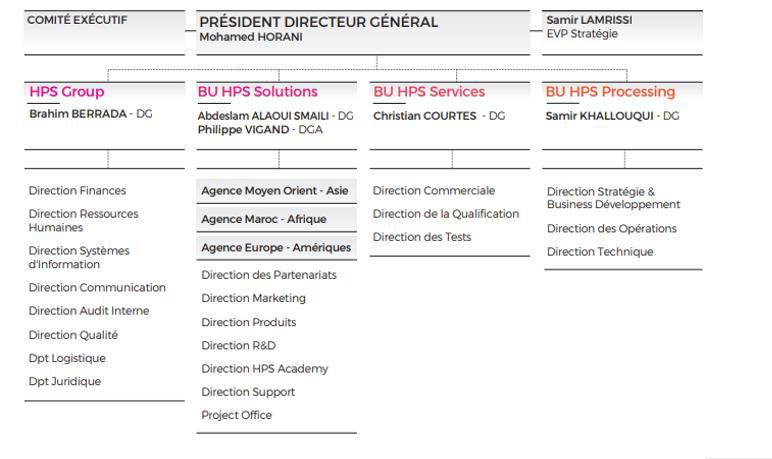
\includegraphics[width=0.6\textwidth]{page12_img02.jpeg}
\caption{Organigramme d'HPS}
\end{figure}

\subsection{HPS Solutions}

Entité historique du Groupe, HPS Solutions conçoit, développe, commercialise, installe et supporte une suite de solutions de paiement électronique multicanal. Leur suite logicielle PowerCARD propose des solutions complètes, paramétrables et évolutives, à même de répondre aux besoins les plus spécifiques des utilisateurs. Évalué « Positive » par le Gartner durant 3 années consécutives, PowerCARD se positionne dans le Top 5 mondial des meilleures solutions de l'industrie monétique.

\subsection{HPS Services}

Au sein du Groupe, les activités de services IT sont portées par HPS Services, qui \oe uvre pour la maîtrise et la performance des systèmes d'informations pour le compte de grands groupes internationaux. HPS Services repose sur la structure et les équipes de la société Acpqualife, créée en 2002 et filiale à 100\% du Groupe HPS depuis 2010.

Les activités de HPS Services se basent sur l'expertise internationale de plus de 75 consultants dans les domaines du test et de la qualification logicielle. HPS Services offre également des services d'assistance à maîtrise d'ouvrage dans le cadre de projets de transformation des SI et des services d'ingénierie IT autour des technologies JEE, Spring, JBOSS, Angular Js ou encore JSF, et associés à l'implémentation de méthodologies de type agile.

\subsection{HPS Processing}

HPS Processing, créée en 2016, met en \oe uvre des moyens humains et matériels, des services à forte valeur ajoutée et son expertise autour de PowerCARD pour offrir à ses clients les solutions du Groupe en mode externalisé. L'activité Processing couvre 3 secteurs d'activité distincts :

\begin{itemize}[leftmargin=*]
\item Le Processing de solutions de paiement qui s'adresse aux institutions financières et opérateurs de paiement pour gérer l'ensemble de leurs activités monétiques.
\item La gestion des activités de Switching à l'échelle nationale ou régionale qui consiste à gérer les demandes d'autorisation et à traiter la compensation des flux entre différents opérateurs.
\item Le Processing de solutions pour les acteurs de micro finance pour la gestion complète de leur activité et la dématérialisation des flux financiers liés au déblocage et au remboursement des crédits.
\end{itemize}

\section{Chiffres clés}

Avec une croissance continue et de récentes acquisitions, HPS Group compte plus de 1 500 collaborateurs et dessert plus de 500 institutions dans plus de 98 pays sur 5 continents.

\begin{table}[H]
\centering
\caption{Chiffres clés d'HPS (2024)}
\begin{tabularx}{0.9\textwidth}{l X}
\toprule
\textbf{Indicateur} & \textbf{Valeur} \\
\midrule
Clients & Plus de 500 \\
Pays & Plus de 98 \\
Continents & 5 \\
Employés & Plus de 1 500 \\
Bureaux & Casablanca, Paris, Aix-en-Provence, Dublin, Dubaï, Jordanie, Singapour, Pune, Sydney, Le Cap, Maurice, Montréal \\
\bottomrule
\end{tabularx}
\end{table}

\section{ACPQUALIFE - HPS Group}

ACPQUALIFE est une société spécialisée dans les systèmes d'informations (SI), particulièrement dans le domaine de test et qualification logicielle, relatif à la monétique et à la gestion des transactions électroniques. ACPQUALIFE met toute son expertise pour des systèmes d'informations performants. Elle s'illustre notamment pour son expertise internationale dans le domaine du Test et de la Qualification logicielle. ACPQUALIFE est un expert des systèmes d'informations, il fournit une offre de services complète et sur-mesure, possède une structure entièrement dédiée aux métiers du test et un centre d'expertise dans le secteur des moyens de paiement électroniques. Elle dispense une formation pragmatique et certifiante.

\section{Historique}

La société ACPQUALIFE a été créée en 2002, suite à la fusion de deux entreprises :
\begin{itemize}[leftmargin=*]
\item ACP (Architect \& Consulting Partners), fondée par M. Christian COURTES, son Directeur Général actuel, en charge des activités services,
\item QUALIFE, spécialisée dans la qualification de systèmes d'information, fondée par M. Marc DURUPT, son Directeur Associé actuel, en charge des expertises sur les métiers du test, en collaboration avec Mme Véronique THEAULT, sa Directrice Associée actuelle, en charge des offres de qualification.
\end{itemize}

En 2010, la société ACPQUALIFE a fusionnée avec le groupe HPS (Hightech Payment Systems), spécialisé dans les paiements électroniques, dont le siège se trouve à Casablanca au Maroc.

\section{Mission}

La société ACPQUALIFE a pour mission principale d'apporter à ses clients des solutions performantes et pérennes ; afin de maîtriser leur système d'information. Et ce, depuis la conception jusqu'à la mise en production, en passant par les phases d'architectures, de réalisations et de tests.

ACPQUALIFE veille sur la sécurité des transactions électroniques, l'adaptabilité simplifiée aux standards internationaux, le développement des solutions mobiles, \ldots

\section{Valeurs (ACPQ)}

ACPQUALIFE fonde son identité et affirme son image auprès de ses clients et collaborateurs à travers quatre valeurs principales :
\begin{itemize}[leftmargin=*]
\item \textbf{Anticipation} : une capacité d'innovation qui permet de proposer aux clients des solutions adaptées et performantes,
\item \textbf{Professionnalisme} : des propositions bâties sur des savoir-faire éprouvés qui sont le résultat d'une capitalisation des expériences,
\item \textbf{Contrôle} : Un développement ancré autour de la culture de l'engagement qui permet une optimisation de la maîtrise des interventions,
\item \textbf{Qualité} : Dans toutes les interventions, application de la démarche « Qualife », qui vise à garantir un véritable label de qualité.
\end{itemize}

\section{Expertises}

Propose une offre de services complète et sur-mesure dont la maîtrise technique est mise au service des activités métiers de ses clients,
\begin{itemize}[leftmargin=*]
\item Maîtrise des réalisations dans le domaine des NTIC et de l'Ingénierie Mobile (Architecture, Méthodologie, Réalisation, Recette)
\item Maîtrise des environnements de production et des processus à mettre en \oe uvre pour garantir leur productivité (Expertise ITIL, Mise en \OE uvre de SLA, Devops, Cloud, Hadoop\ldots)
\item Expertise dans le domaine des Tests et de la Qualification Logicielle : Conseil, Formation, Mise en \OE uvre, Assistance MOA 2 et MOE3, Expertise Outils, Tierce Recette Applicative.
\end{itemize}

\section{Services}

\begin{itemize}[leftmargin=*]
\item \textbf{Maîtrise d'ouvrage AMOA} : ACPQUALIFE est un partenaire qui apporte des idées innovantes dans le cadre des évolutions et de la transformation des SI, en s'appuyant sur une parfaite connaissance du secteur métier ainsi que sur son expertise technique et méthodologique,
\item \textbf{Qualification} : ACPQUALIFE possède un département entièrement dédié aux métiers du test. Il s'appuie notamment sur « Qualitest », une méthodologie pragmatique, rodée et adaptable,
\item \textbf{Ingénierie d'Infrastructure} : ACPQUALIFE accompagne ses clients dans la continuité de services et la performance de leur Système d'Information,
\item \textbf{Ingénierie IT} : Au travers d'une activité concentrée sur les Nouvelles Technologies de l'Information et des Communications, ACPQUALIFE a acquis une spécialisation reconnue dans la réalisation d'applications en Architectures.
\end{itemize}

\section{Chiffres Clés}

\begin{table}[H]
\centering
\caption{Chiffres clés ACPQUALIFE - HPS Group}
\begin{tabularx}{0.9\textwidth}{l X}
\toprule
\textbf{ACPQUALIFE - HPS Group} & \\
\midrule
Adresse & ACPQUALIFE, 805 Av. J.R.G Gautier De La Lauzière 13290 Aix En Provence - France \\
Activité & Gestion d'installations informatiques \\
Forme juridique & Société par actions simplifiée \\
Date immatriculation & Le 09-07-2002 \\
Tranche d'effectif & 50 à 99 salariés \\
Chiffre d'affaires 2016 & 12 938 700,00 \euro \\
Implantation & Aix en Provence, Paris, Toulouse, Lausanne, Lille et Sophia Antipolis. \\
\midrule
\multicolumn{2}{l}{Plus de 100 consultants} \\
\multicolumn{2}{l}{Plus 28\% de croissance} \\
\multicolumn{2}{l}{Plus de 25\% d'activité à l'international} \\
\bottomrule
\end{tabularx}
\end{table}

\vspace{10pt}
\textbf{Conclusion}

En somme, HPS et sa filiale ACPQUALIFE constituent un environnement hautement spécialisé et exigeant, dédié à la performance et à la sécurité des systèmes d'information monétiques. L'expertise internationale du groupe et sa culture de la qualité fournissent un cadre idéal pour l'apprentissage et l'application des meilleures pratiques en ingénierie logicielle. La compréhension de cette organisation permet de mieux appréhender les défis techniques et opérationnels du projet d'automatisation des tests, dont le contexte et les objectifs spécifiques seront détaillés dans le chapitre suivant.


% ── Chapitre II: Contexte et problématique ──
% ══════════════════════════════════════════════════════════════════
% CHAPITRE II — Contexte et problématique
% ══════════════════════════════════════════════════════════════════
\newpage
\chapter{Contexte et problématique}
\vspace{1cm}
\minitoc
\newpage

\textit{La présentation et la gestion du projet revêt un caractère important pour la suite du rapport. La description du contexte, de la problématique, des missions et de la gestion du projet nous permet de mieux comprendre sa réalisation et sa concrétisation.}

\vspace{10pt}
\textbf{Introduction}

La complexité croissante des solutions monétiques comme PowerCARD nécessite une gestion de projet rigoureuse et des processus de validation infaillibles. Dans un contexte multi-clients où les mêmes modules logiciels sont déployés avec des paramétrages spécifiques, le risque de régression lors des mises à jour est élevé. Ce chapitre présente le contexte spécifique du projet de stage, en détaillant la problématique liée aux tests manuels répétitifs, les objectifs fixés pour l'automatisation des processus de validation, ainsi que la planification et la gestion du projet adoptées pour mener à bien cette mission.
\vspace{10pt}

L'usage de l'informatique s'est généralisé dans tous les secteurs d'activité. Le secteur de la monétique, qui connait une très forte évolution de son périmètre, de ses applications et de ses usages, s'accompagne de vulnérabilités qui n'existaient pas avec le paiement de proximité. Les paiements électroniques sont caractérisés par trois éléments constitutifs :

\begin{itemize}[leftmargin=*]
\item Un élément technique, consistant à l'utilisation des procédés informatiques, magnétiques, électroniques et télématiques au lieu du papier,
\item Un élément monétique, à savoir la circulation de la monnaie d'un compte à un autre de manière instantanée,
\item Un élément organique, impliquant l'intervention des banques, du commerce et consommateurs pour la mise en \oe uvre des paiements électroniques.
\end{itemize}

Dans la partie présentation de la société, nous avons vu que HPS apporte des solutions logicielles standards PowerCARD qui assurent la sécurité et la fiabilité dans le processus de la monétique. Etant donné que l'entreprise commercialise ses solutions à l'international, les clients demandent une adaptation (modification) de la solution en termes de fonctionnalités par rapport à leurs besoins spécifiques.

HPS s'occupe plusieurs projets de même client (banque internationale) notamment dans des zones géographiques différents, ces projets partagent des parties de code commun. Donc on est dans l'obligation de maîtriser les impacts qui pouvant résulter des changements associés aux évolutions et corrections de code entre chaque projet. Il est devenu indispensable de réaliser des campagnes de test automatisé qui détectent les futures régressions.

Mon projet s'inscrit dans ce contexte critique d'Assurance Qualité (QA). Bien que les étapes de test manuel soient maîtrisées et exécutées normalement, la charge de travail répétitive qu'elles imposent pousse vers l'automatisation. Cependant, l'automatisation classique avec des outils comme Cypress exige des compétences avancées en programmation Javascript, créant un goulet d'étranglement pour les testeurs fonctionnels. C'est ici qu'intervient la véritable valeur ajoutée de ce projet : concevoir et développer une solution innovante, le « QA Cypress Generator Dashboard », visant à automatiser le processus de création des tests automatisés eux-mêmes, sans écrire une seule ligne de code.

\section{Missions et objectifs}

Les missions et objectifs de mon stage sont comme suit :

\begin{itemize}[leftmargin=*]
\item Identification et capture des exigences client, fonctionnelles, techniques et standards,
\item Préparation du plan de tests,
\item Identification et conception des cas de tests,
\item Préparation des jeux de données des tests,
\item Implémentation des cas de tests step-to-step,
\item Assurance de la couverture totale des exigences,
\item Préparation et exécution des campagnes de tests,
\item Automatisation des cas de test.
\end{itemize}

Certes, un projet de stage est susceptible de changement en fonction des imprévus, délais et résultats attendus. La phase de réalisation représente l'aboutissement des objectifs décrits et fixés auparavant. Elle doit être bien planifiée en fonction des tâches à effectuer et des temps alloués.

\section{Cahier de charges}

Pour effectuer un stage de PFE, il faut bien entendu une entreprise, un stagiaire, une mission, un délai, un encadrement ainsi que des besoins légitimes pour la réalisation de ce projet.

\begin{table}[H]
\centering
\caption{Cahier de charges du stage}
\begin{tabularx}{0.9\textwidth}{l X}
\toprule
\textbf{Rubrique} & \textbf{Détails} \\
\midrule
Entreprise & HPS \\
Adresse & Casablanca Nearshore, Shore 3 - Sector A \\
Contact & Fax 05290-45000 \\
Stagiaire & Mohamed KARKACHI, Ingénieure d'état en informatique et réseaux \\
Durée & De 01 Mars Au 31 Aout. 2022 \\
Encadrement & Mme. Salima MISSOUR, HPS / Mr. Ali IDMANSOUR, (Université EMSI) \\
\bottomrule
\end{tabularx}
\end{table}

Pour la réalisation de ce projet, il est normal de mettre à la disposition du stagiaire un ensemble de moyens matériel, logiciels et financiers.

\begin{itemize}[leftmargin=*]
\item[$\checkmark$] \textbf{Moyens matériels} : Un PC portable et un écran supplémentaire configuré ``entreprise'' qui permet un certain nombre de privilèges de manipulation, d'accéder aux logiciels, outils et bases de données requises, \ldots
\item[$\checkmark$] \textbf{Moyens logiciels} : Des outils de travail de la société, accompagnés d'une formation et documentation, sont nécessaires pour la réalisation du projet de Fin d'études.
\item[$\checkmark$] \textbf{Moyens financiers} : Des gratifications mensuelles qui permettent au stagiaire de supporter les frais de logement, transport, restauration, ...
\end{itemize}

\section{Planning global du stage}

Afin de réaliser ma mission, il fallait de suivre une suite de formation sur les bases de la chaîne monétique et les outils de tests utilisés par l'entreprise, analyser les cahiers spécification du chaque composant, faire la conception des tests, élaborer un scénario de test, l'exécution manuellement de ce scénario puis l'automatisation.

Tout au long de cette période de stage, j'avais trois réunions par semaine avec mon équipe pour discuter de mon avancement et les difficultés rencontrées. La figure ci-dessous représente le diagramme de GANTT de mon projet, en illustrant les différentes tâches réalisées.

\begin{figure}[H]
\centering
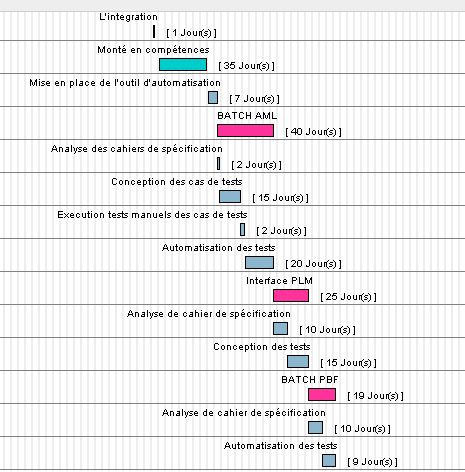
\includegraphics[width=\textwidth]{page18_img02.png}
\caption{Diagramme de Gantt}
\end{figure}

\section{Gestion du projet}

\subsection{Description}

Le client utilisera les solutions standards PowerCARD suivantes :
\begin{itemize}[leftmargin=*]
\item PowerCARD Issuer,
\item PowerCARD switch.
\end{itemize}

Mon projet de stage concernera les tests menés sur les changements effectués au niveau la solution PowerCARD Issuer.

\subsection{Organisation de projets}

\begin{figure}[H]
\centering
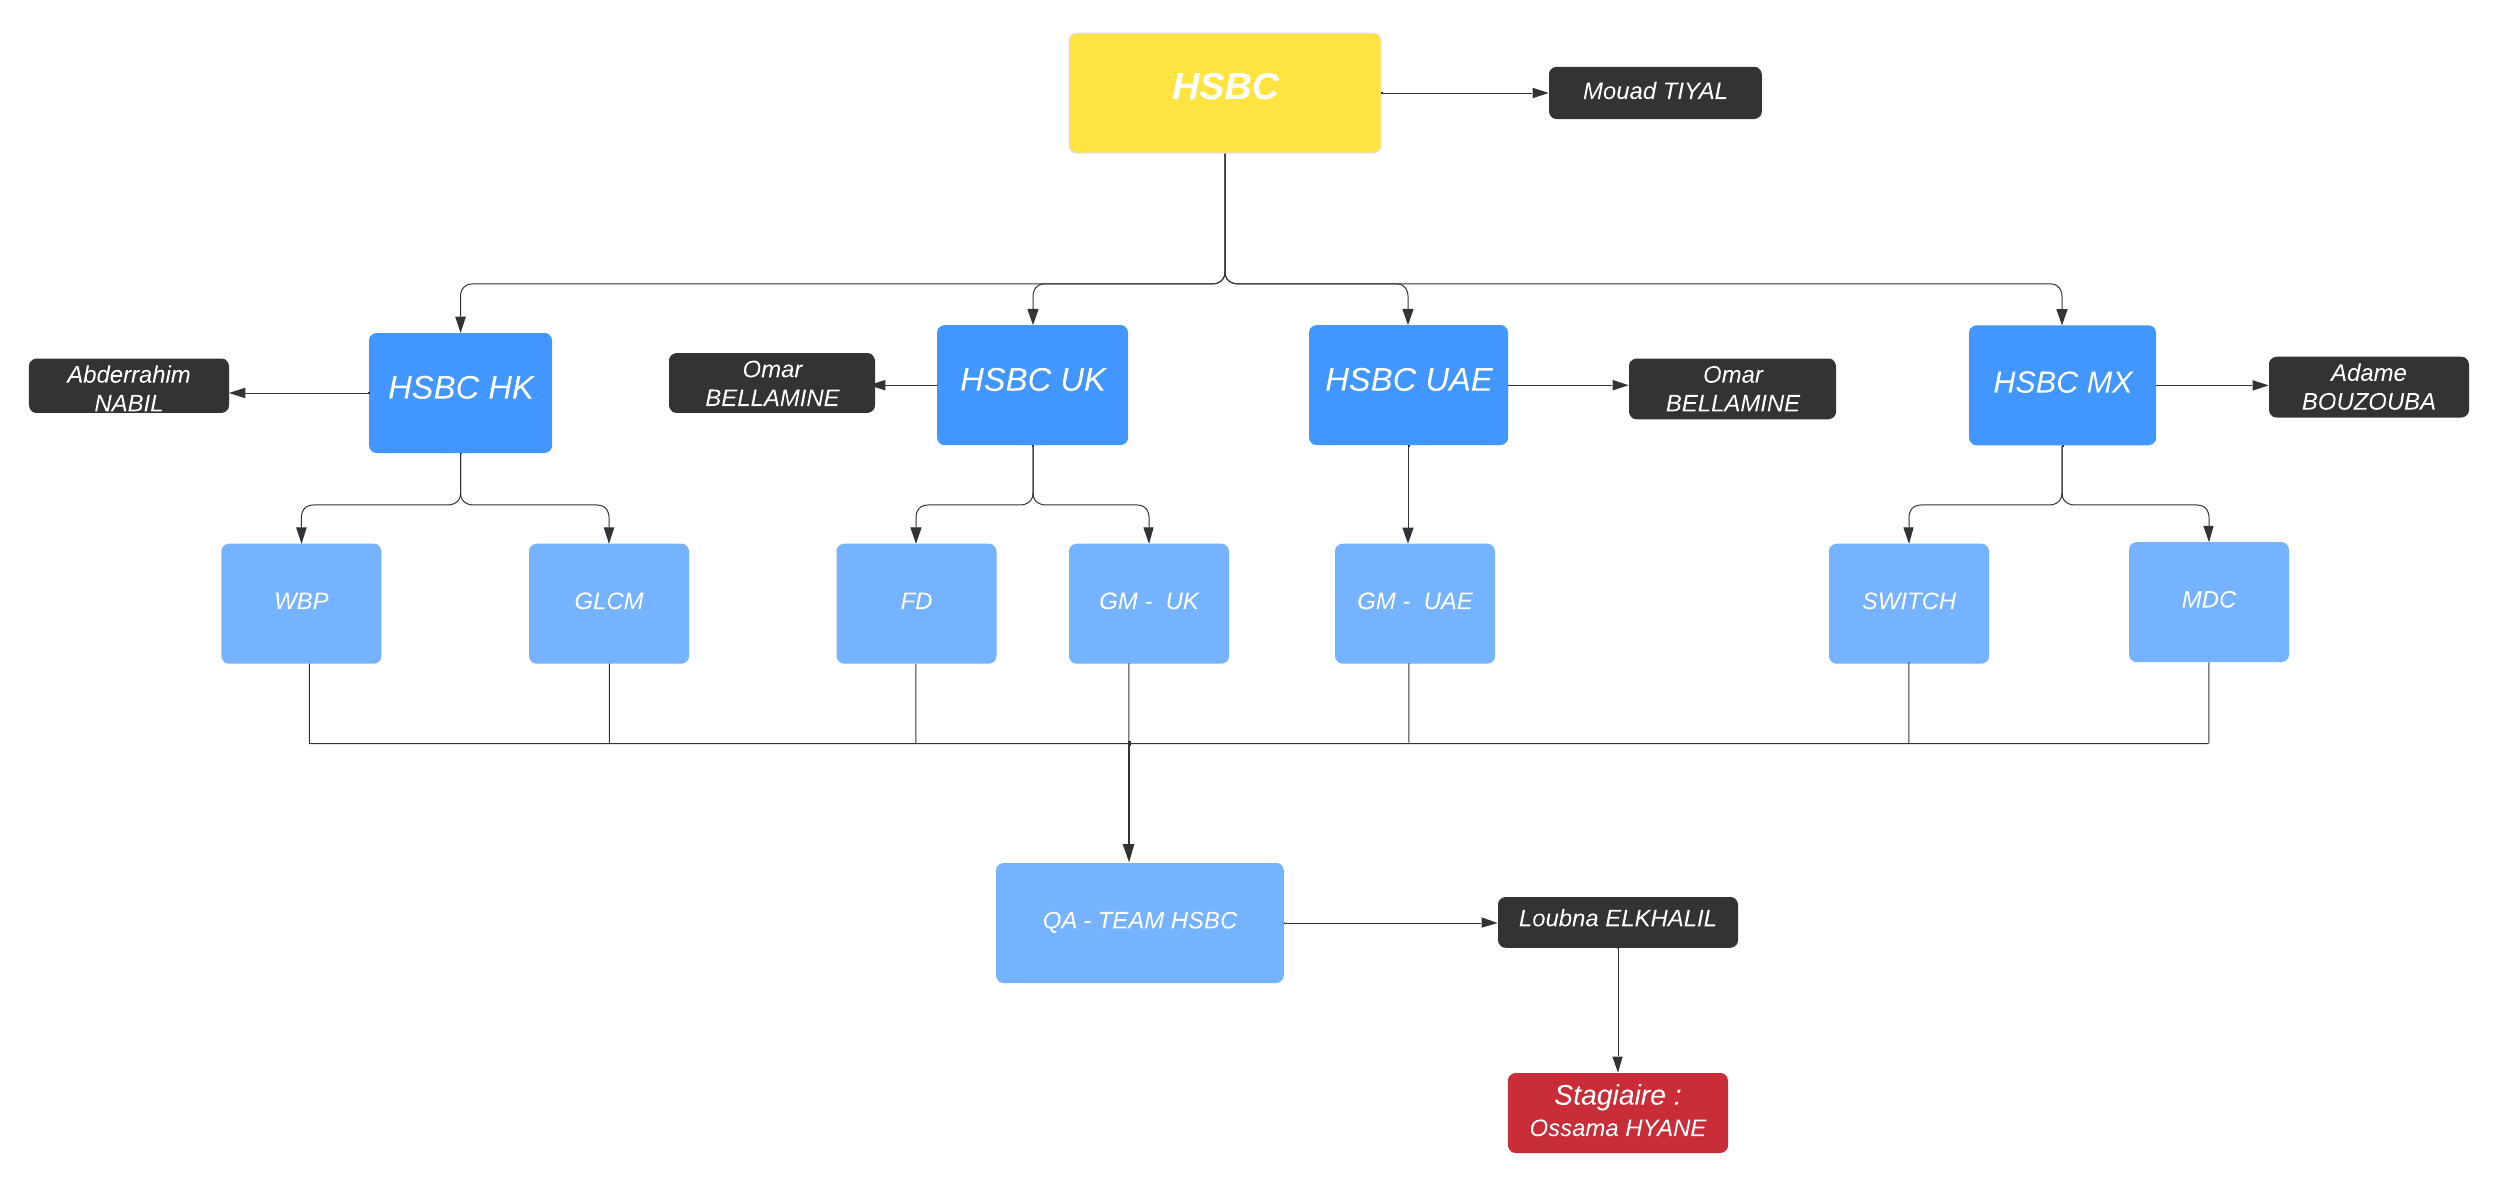
\includegraphics[width=0.7\textwidth]{page19_img02.png}
\caption{Décomposition de projets}
\end{figure}

\subsection{Livrables projet}

\begin{table}[H]
\centering\footnotesize
\caption{Livrables projet}
\begin{tabularx}{\textwidth}{l X X X}
\toprule
\textbf{Livrables} & \textbf{Données d'entrée} & \textbf{Étapes} & \textbf{Données de sortie} \\
\midrule
Définition des exigences & Documents de spécifications BSD, BRD et TSF, planning de projet. & Révision et analyse des documents, Saisie des exigences sous l'outil, Définition des criticités et priorités & Gestion des exigences \\
\midrule
Conception des tests & Documents de spécifications. & Identification des conditions de test, Conception et rédaction des cas de test, Préparation des jeux de données & Cas de test, Plan de test, Campagne de test \\
\midrule
Exécution des tests & Documents de spécifications, Scénarios de test, Cas de test, Campagne de test & Exécution des campagnes, Enregistrement des résultats, Comparaison des résultats & Fiches d'anomalies, Rapport de synthèse de test \\
\midrule
Automatisation des tests & Jeux de données, Scripts d'automatisation & Identification des objectifs, Analyse de faisabilité, Configuration de l'environnement & Résultats des tests automatisés \\
\midrule
Suivi du déroulement des tests & Données d'anomalies, Données de couverture, Preuves de test & Mesure et analyse des résultats, Suivi du progrès & Leçons retenues, Améliorations \\
\bottomrule
\end{tabularx}
\end{table}

\vspace{10pt}
\textbf{Conclusion}

La définition claire du contexte, des objectifs et des livrables a permis d'établir une feuille de route solide pour la réalisation de ce projet. La transition vers une automatisation accrue des tests répond directement à la problématique de fiabilité et de gain de temps identifiée par HPS. Afin de concrétiser ces objectifs, il est indispensable de s'appuyer sur des bases méthodologiques reconnues et des outils performants. Le chapitre suivant exposera le cadre théorique du cycle de développement logiciel et les méthodologies de test adoptées pour structurer techniquement notre démarche.


% ── Chapitre III: Méthodologies et outils ──
% ══════════════════════════════════════════════════════════════════
% CHAPITRE III — Méthodologies et outils
% ══════════════════════════════════════════════════════════════════
\newpage
\chapter{Méthodologies et outils}
\vspace{1cm}
\minitoc
\newpage

\textit{Ce chapitre se propose de donner un aperçu sur les tests logiciel ; les méthodologies suivies pour la réalisation du projet ; les étapes des tests effectuées, depuis les exigences jusqu'à l'automatisation, ainsi que les technologies innovantes intégrées (IA et orchestration de workflows).}

\vspace{10pt}
\textbf{Introduction}

La réussite d'un projet d'automatisation des tests repose fondamentalement sur la rigueur des méthodes employées et l'adéquation des outils choisis. Ce chapitre aborde les concepts théoriques sous-jacents à notre travail, en mettant l'accent sur le cycle de développement logiciel en V itératif, particulièrement adapté aux exigences de traçabilité du secteur bancaire. Nous détaillerons également les différentes phases du processus de test, allant de la gestion des exigences à l'exécution et au suivi des anomalies. Enfin, nous présenterons les technologies innovantes intégrées dans notre solution : l'intelligence artificielle (Mistral AI) pour la découverte automatique d'écrans et la génération de tests, ainsi que l'outil d'orchestration n8n pour l'automatisation des workflows de préparation de données.
\vspace{10pt}

Un cycle de vie d'un projet informatique est le descriptif du processus à suivre pour mener à bien le projet. Le processus décrit les phases à réaliser pour atteindre les objectifs fixés. Le processus de test au sein des projets PowerCARD adopte un cycle itératif.

\begin{figure}[H]
\centering
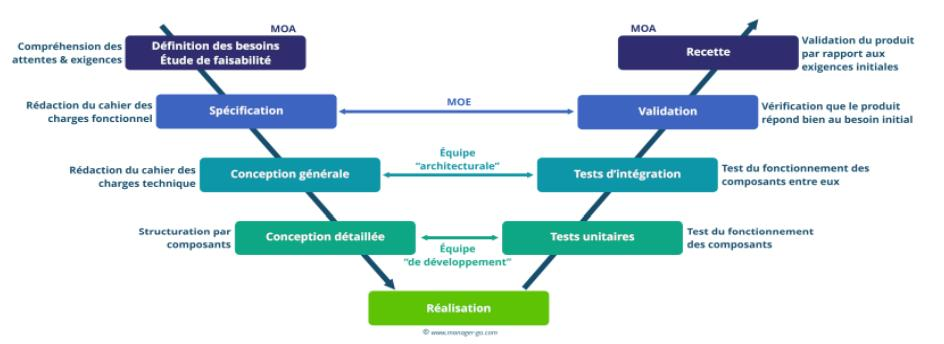
\includegraphics[width=0.7\textwidth]{page22_img02.jpeg}
\caption{Cycle en V}
\end{figure}

Le problème avec le cycle en V est sa rigidité. Afin d'adopter cette souplesse, le projet sur lequel on travaille a opté pour un cycle en V itératif.

\begin{figure}[H]
\centering
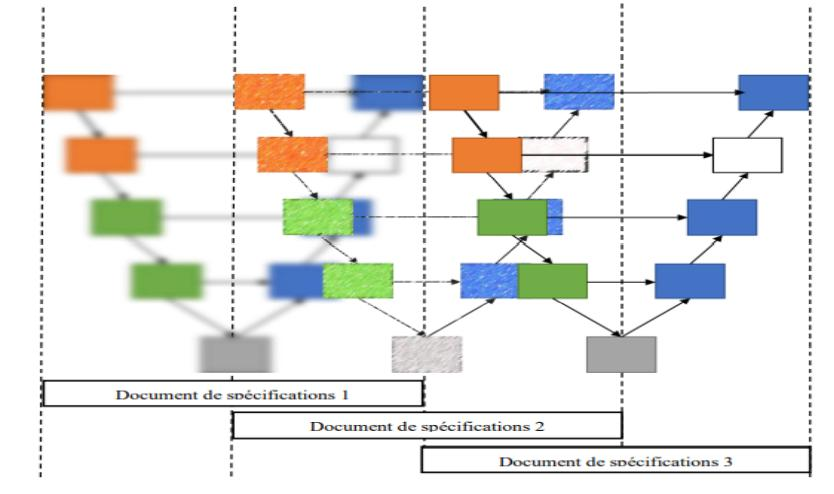
\includegraphics[width=0.8\textwidth]{page23_img02.jpeg}
\caption{Exemple de cycle en V itératif d'un Sprint de 3 documents de spécifications}
\end{figure}

\section{Périmètre et méthodes}

Un test est un ensemble de cas à tester. En général, le test logiciel est un procédé de validation et de vérification permettant de s'assurer que le produit est conforme à ses spécifications.

Les niveaux de test identifiés pour le projet sont :
\begin{itemize}[leftmargin=*]
\item \textbf{Tests systèmes}, qui permettent de traiter le comportement d'un système/logiciel complet.
\item \textbf{Tests de non-régression}, qui permettent de valider qu'une mise à jour d'un module du logiciel n'a pas provoqué un problème dans un module qui n'a pas été modifié.
\end{itemize}

\begin{figure}[H]
\centering
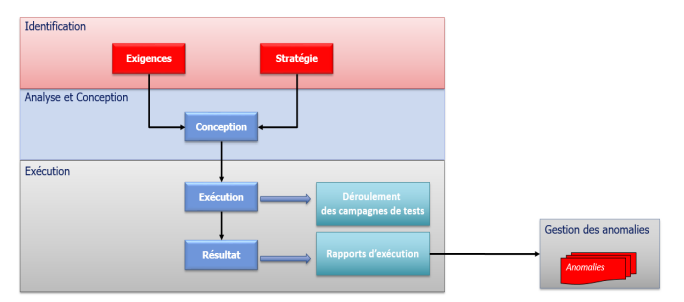
\includegraphics[width=0.6\textwidth]{page24_img02.png}
\caption{Méthodologie de test}
\end{figure}

\section{Tests manuels et automatisés}

\subsection{Tests manuels}

Un test manuel est un test exécuté par un testeur. Il est effectué dès la réception des livrables. Il permet d'exécuter manuellement les tests.

\subsection{Tests automatisés}

Un test automatisé est un test dont l'exécution ne nécessite pas l'intervention d'un testeur. L'exécution des tests automatisés requiert donc l'utilisation de solutions informatiques.

\begin{figure}[H]
\centering
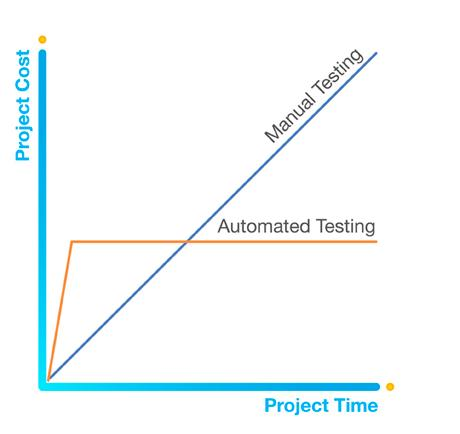
\includegraphics[width=0.7\textwidth]{page26_img02.jpeg}
\caption{Coût des tests manuels par rapport aux tests automatisés}
\end{figure}

\section{Etapes du projet}

\subsection{Gestion des exigences}

Une exigence représente l'expression de ce qui doit être implémenté dans une application. Une bonne exigence doit être : Abstraite, Non ambiguë, Traçable, Testable.

\begin{figure}[H]
\centering
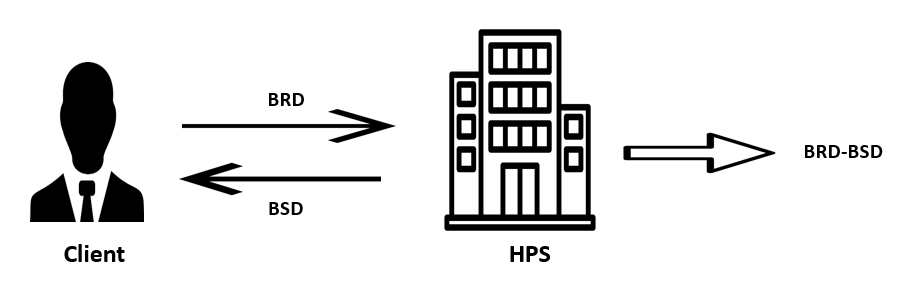
\includegraphics[width=0.7\textwidth]{page27_img02.png}
\caption{Elaboration du document de spécifications}
\end{figure}

\subsection{Conception des tests}

\begin{figure}[H]
\centering
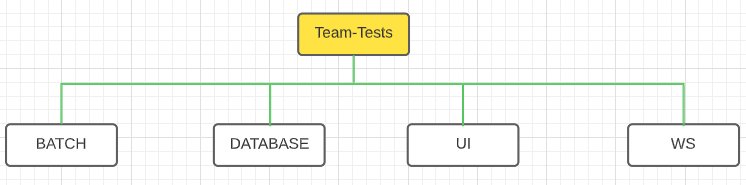
\includegraphics[width=0.7\textwidth]{page28_img02.png}
\caption{Organisation des tests dans les projets PowerCARD}
\end{figure}

\subsection{Exécution des tests}

Les intervenants sur cette phase auront pour charge de « dérouler » les cas de test dans l'ordre défini (campagne de test), puis, vérifier les résultats.

\subsection{Gestion des anomalies}

\begin{figure}[H]
\centering
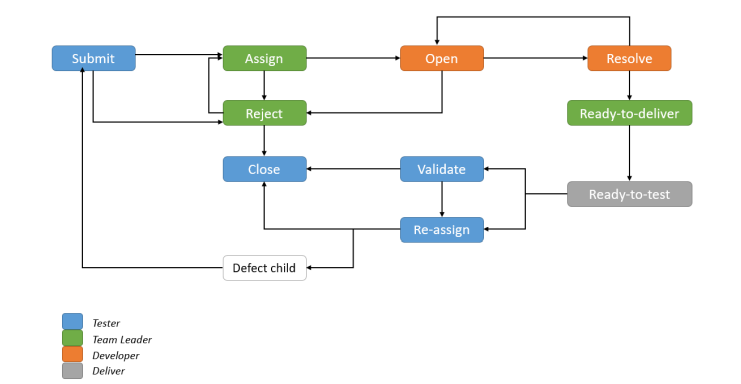
\includegraphics[width=0.7\textwidth]{page31_img02.png}
\caption{Cycle de vie d'une anomalie}
\end{figure}

\begin{itemize}[leftmargin=*]
\item \textbf{Submit} : représente une anomalie nouvellement créée,
\item \textbf{Assign} : anomalie assignée à la personne qui s'occupera de sa correction,
\item \textbf{Reject} : anomalie rejetée (redondance, non reproductible, etc.),
\item \textbf{Open} : anomalie en cours de traitement/correction,
\item \textbf{Resolve} : anomalie corrigée,
\item \textbf{Ready-to-deliver} : anomalie prête à être livrée,
\item \textbf{Ready-to-test} : anomalie prête à être re-testée,
\item \textbf{Validate} : approbation et validation de la correction,
\item \textbf{Re-assign} : anomalie réassignée car non corrigée correctement,
\item \textbf{Close} : anomalie fermée, corrigée et validée.
\end{itemize}

\subsection{Automatisation des tests}

Les tests fonctionnels manuels suivent un processus normal et maîtrisé (conception, exécution, suivi). Cependant, pour éviter la régression lors des livraisons continues, ils doivent être exécutés très régulièrement. C'est ici que la différence se fait : l'automatisation devient obligatoire. Mais coder des scripts E2E complexes en Cypress prend du temps et demande un profil technique de développeur.

\textbf{La Solution : QA Cypress Dashboard}

Pour combler le fossé entre les testeurs fonctionnels et l'automatisation technique, la solution développée durant ce stage est le \textbf{Cypress Generator Dashboard}. Ce portail Web interactif permet aux testeurs de naviguer visuellement dans les modules de PowerCARD, de renseigner les données via des formulaires, et de laisser le système générer instantanément et de façon autonome les scripts Cypress (.cy.js) et les jeux de données JSON. Le Dashboard est donc la solution d'automatisation ultime développée pour résoudre la problématique de la barrière technique.

\subsection{Suivi du déroulement des tests}

Cette activité se déroule tout au long de l'étape d'exécution de la recette fonctionnelle.

% ══════════════════════════════════════════════════════════════════
% SECTION: Intelligence Artificielle dans le Testing
% ══════════════════════════════════════════════════════════════════
\section{Intelligence Artificielle dans le Testing}

L'intégration de l'intelligence artificielle dans le processus de test représente une avancée majeure. Dans notre projet, nous utilisons \textbf{Mistral AI}, un modèle de langage de grande taille (LLM), pour automatiser deux tâches critiques :

\subsection{Découverte automatique d'écrans (AI Discovery)}

Le processus de découverte automatique fonctionne en trois étapes :

\begin{enumerate}
\item \textbf{Crawling Cypress} : Un script Cypress parcourt automatiquement tous les modules de PowerCARD (Acquirer, System, Issuer, Switch, Fraud, xPOS). Pour chaque écran, il extrait les champs de formulaire (inputs, selects, textareas), les boutons, et les métadonnées de l'interface.

\item \textbf{Analyse IA (Mistral)} : Les schémas bruts extraits sont envoyés à l'API Mistral qui les analyse pour :
\begin{itemize}[leftmargin=*]
\item Classifier chaque écran dans le bon module et workspace,
\item Générer des labels lisibles (ex: \texttt{switch-merchant-onboarding} $\rightarrow$ ``Switch - Merchant Onboarding''),
\item Identifier le type d'écran (CRUD, recherche, configuration),
\item Suggérer la meilleure stratégie de sélecteur Cypress pour chaque champ.
\end{itemize}

\item \textbf{Enrichissement du catalogue} : Les écrans enrichis sont fusionnés avec le catalogue existant (\texttt{projectCatalog.json}), créant un référentiel complet et à jour.
\end{enumerate}

\subsection{Génération de tests par IA}

Le service \texttt{generator-service} (port 8002) expose deux endpoints d'IA :

\begin{itemize}[leftmargin=*]
\item \texttt{POST /api/generate-ai-test} : Génère un script Cypress complet pour un écran donné, en injectant le contexte du projet (Page Objects, Custom Commands, conventions).
\item \texttt{POST /api/generate-ai-flow} : Génère un test multi-étapes pour un flux fonctionnel complet (ex: cycle de vie terminal, onboarding marchand).
\end{itemize}

Le modèle utilisé est \textbf{mistral-large-latest} avec une température basse (0.1) pour garantir la cohérence et la reproductibilité du code généré.

% ══════════════════════════════════════════════════════════════════
% SECTION: Orchestration avec n8n
% ══════════════════════════════════════════════════════════════════
\section{Orchestration avec n8n}

\textbf{n8n} est un outil d'automatisation de workflows open-source qui permet de créer des chaînes de traitement de données via une interface visuelle ``no-code''. Dans notre projet, n8n est utilisé pour orchestrer les tâches de préparation de données et d'archivage.

\subsection{Workflow de préparation des données}

Le workflow ``Automated Data Prep \& DB Archiving'' implémente le flux suivant :

\begin{enumerate}
\item \textbf{Trigger} : Déclenchement manuel ou planifié.
\item \textbf{Génération de carte de test} : Appel à l'endpoint \texttt{GET /api/connect/random-test-card} pour récupérer une carte de test valide depuis l'API PowerCard Connect.
\item \textbf{Création de la table} : Vérification et création de la table \texttt{generated\_test\_cards} dans SQLite si elle n'existe pas.
\item \textbf{Insertion} : Stockage du numéro de carte et du type dans la base de données avec horodatage automatique.
\item \textbf{Vérification} : Requête de vérification pour confirmer l'insertion (5 dernières entrées).
\end{enumerate}

\subsection{Avantages de l'approche n8n}

\begin{itemize}[leftmargin=*]
\item \textbf{Visuel et accessible} : Les testeurs QA peuvent créer et modifier des workflows sans coder.
\item \textbf{Extensible} : Plus de 400 n\oe{}uds natifs pour intégrer d'autres outils (Jira, Slack, email).
\item \textbf{Planifiable} : Exécution automatique via des déclencheurs temporels (cron).
\item \textbf{Reproductible} : Les workflows sont exportés en JSON et versionnés dans le dépôt Git.
\end{itemize}


% ══════════════════════════════════════════════════════════════════
% SECTION: Environnement technologique et outils
% ══════════════════════════════════════════════════════════════════
\section{Environnement technologique et outils}

Pour mener à bien les différentes phases de ce projet, de la conception des tests jusqu'au développement de la solution d'automatisation finale, un ensemble d'outils performants et de technologies modernes a été déployé.

\subsection{Outils d'Automatisation et de Tests API}
\begin{itemize}[leftmargin=*]
\item \textbf{Cypress} : Framework de test de bout en bout moderne utilisé pour l'automatisation des tests fonctionnels de l'interface utilisateur de PowerCARD. Il permet une exécution rapide et offre un rapport visuel détaillé.
\item \textbf{Postman} : Outil de collaboration pour le développement d'API, utilisé pour interagir avec les endpoints de PowerCARD (comme Connect API), comprendre les requêtes et préparer les jeux de données.
\item \textbf{Newman} : L'outil en ligne de commande de Postman, indispensable pour exécuter et automatiser les collections Postman directement depuis le terminal.
\end{itemize}

\subsection{Outils de Développement du Dashboard}
\begin{itemize}[leftmargin=*]
\item \textbf{React 18.3 \& Vite 5.4} : Bibliothèques et outils de build utilisés pour créer une interface utilisateur rapide, réactive et ergonomique pour le Dashboard.
\item \textbf{Node.js 22 LTS} : Utilisé côté serveur pour créer les microservices du Dashboard, interagir avec le système de fichiers et servir de proxy sécurisé.
\item \textbf{Monaco Editor} : L'éditeur de code de VS Code, intégré dans le Dashboard pour la visualisation et l'édition du code généré avec coloration syntaxique.
\item \textbf{SQLite} : Base de données locale légère utilisée par l'équipe QA pour gérer les configurations et les cartes de test.
\end{itemize}

\subsection{Intelligence Artificielle et Orchestration}
\begin{itemize}[leftmargin=*]
\item \textbf{Mistral AI} : Modèle de langage utilisé pour la découverte automatique d'écrans et la génération de scripts de test. Modèle \texttt{mistral-large-latest} via API REST.
\item \textbf{n8n} : Outil d'automatisation de workflows open-source pour l'orchestration des tâches de préparation de données et d'archivage dans la base SQLite.
\end{itemize}

\subsection{Infrastructure et DevOps}
\begin{itemize}[leftmargin=*]
\item \textbf{Docker \& Docker Compose} : Containerisation de l'ensemble des microservices avec orchestration des dépendances et health checks automatiques.
\item \textbf{Git \& GitHub} : Plateforme de contrôle de version pour la gestion du code source de l'ensemble du projet.
\end{itemize}

\subsection{Collaboration et Gestion de Projet}
\begin{itemize}[leftmargin=*]
\item \textbf{Jira} : Utilisé pour le suivi des anomalies (Bug Tracking) et la gestion des tâches au sein de l'équipe QA.
\end{itemize}

\begin{table}[H]
\centering
\caption{Stack technologique complète du projet}
\renewcommand{\arraystretch}{1.3}
\begin{tabularx}{\textwidth}{l l X}
\toprule
\textbf{Composant} & \textbf{Technologie} & \textbf{Version / Détail} \\
\midrule
\rowcolor{primary!5} Frontend & React + Vite & 18.3 / 5.4 \\
Code Editor & Monaco Editor & Dernière version \\
\rowcolor{primary!5} Microservices & Node.js (raw \texttt{http}) & 22 LTS \\
Test Framework & Cypress & 15.13.1 \\
\rowcolor{primary!5} IA & Mistral AI API & mistral-large-latest \\
Orchestration & n8n & Dernière version \\
\rowcolor{primary!5} Base de données & SQLite & 3.x \\
Containerisation & Docker + Compose V2 & node:22-alpine \\
\rowcolor{primary!5} Logging & JSON structuré (stdout) & Interne \\
\bottomrule
\end{tabularx}
\end{table}


\vspace{10pt}
\textbf{Conclusion}

La maîtrise des cycles de test et l'utilisation de méthodologies structurées assurent une validation exhaustive des solutions logicielles. L'automatisation, en particulier, s'impose comme une nécessité pour fiabiliser les processus de non-régression tout en optimisant les coûts et les délais. L'intégration de l'intelligence artificielle (Mistral AI) et de l'orchestration de workflows (n8n) positionne notre solution comme un outil de nouvelle génération dans le domaine de l'assurance qualité. Forts de cette base méthodologique et technologique, nous avons pu passer à la phase de concrétisation. Le chapitre suivant présentera en détail les travaux techniques réalisés durant ce stage, incluant l'automatisation effective des scénarios de test ainsi que la conception et la démonstration du Dashboard.


% ── Chapitre IV: Travaux réalisés ──
% ══════════════════════════════════════════════════════════════════
% CHAPITRE IV — Travaux réalisés
% ══════════════════════════════════════════════════════════════════
\newpage
\chapter{Travaux réalisés}
\vspace{1cm}
\minitoc
\newpage

\textit{Ce chapitre détaille les travaux techniques réalisés durant mon projet de fin d'études. Il met en évidence deux grands axes de réalisation : la conception et le développement du « Cypress Generator Dashboard » avec une démonstration pratique complète sur le flux MOTO, et l'automatisation des scénarios de test fonctionnels sur le système PowerCARD.}

\vspace{10pt}
\textbf{Introduction}

Ce chapitre constitue le cœur technique du projet et s'articule autour de la mise en pratique de l'automatisation des tests fonctionnels de bout en bout (E2E). Dans une première partie, nous détaillerons la conception, l'architecture et le développement d'un outil interne innovant : le « Cypress Generator Dashboard ». Cet outil, conçu avec l'écosystème React et Node.js, répond au besoin critique d'abstraire la complexité d'écriture du code Cypress, offrant ainsi à l'équipe qualité une interface intuitive pour auto-générer, configurer et exécuter les campagnes de tests automatisées avec une efficacité décuplée. Dans une seconde partie, nous présenterons un rapport d'exécution technique illustrant l'automatisation de flux métiers complexes sur le système PowerCARD.


% ══════════════════════════════════════════════════════════════════
% SECTION 1: ARCHITECTURE ET DIAGRAMMES UML
% ══════════════════════════════════════════════════════════════════
\newpage
\section{QA Cypress Dashboard --- Conception et Architecture}

\textit{Cette section présente la conception complète du framework d'automatisation de tests E2E développé pour l'application PowerCard v4 --- architecture, diagrammes UML, tous réalisés en TikZ.}

\vspace{10pt}

\begin{tcolorbox}[colback=primary!5, colframe=primary, title=Résumé du Projet Dashboard, arc=5pt]
Analyse architecturale complète du framework d'automatisation de tests E2E pour l'application PowerCard v4 --- diagrammes UML, architecture microservices, et démonstration visuelle de la plateforme.

\vspace{5pt}
\textbf{Métadonnées du projet :}
\begin{itemize}[leftmargin=1.5em]
    \item 32 Écrans Catalogués
    \item 5 API Endpoints
    \item 15 Templates Manuels
    \item 1585 Lignes React
\end{itemize}
\end{tcolorbox}

% ─── Contexte du Projet ───
\subsection{Contexte du Projet}
Le projet \textbf{qa-cypress-e2e} est un framework d'automatisation de tests End-to-End pour l'application bancaire \textbf{PowerCard v4}. Le module \textbf{Dashboard} est une interface React locale qui accélère la création et l'exécution de specs Cypress.

\subsubsection*{Objectif}
Automatiser les tests fonctionnels des écrans PowerCard (Switch, Issuer) en générant des specs Cypress et des fixtures JSON à partir d'une interface graphique intuitive.

\subsubsection*{Utilisateurs}
Équipe QA / Testeurs qui ont besoin de créer rapidement des scénarios de tests sans écrire du code Cypress manuellement.

\subsubsection*{Livrables}
Dashboard React + Vite, scripts de génération automatique, API d'export vers le projet, terminal d'exécution intégré avec rapport visuel.

% ─── Architecture Globale ───
\newpage
\subsection{Architecture Globale}
Vue d'ensemble de l'architecture du système, montrant les interactions entre le dashboard React, le serveur API, le projet Cypress, et l'API PowerCard Connect.

\begin{figure}[H]
\centering
\resizebox{\textwidth}{!}{%
\begin{tikzpicture}[node distance=1.2cm and 1.8cm]
  % ── Frontend Layer ──
  \node[ndBlue, minimum width=4cm, minimum height=1.2cm] (react) {\textbf{React + Vite}\\\footnotesize Port 5175};
  \node[ndBlue, minimum width=2.8cm, right=1cm of react] (monaco) {Monaco Editor};
  \node[ndBlue, minimum width=2.8cm, right=0.5cm of monaco] (forms) {Formulaires\\Dynamiques};
  \node[ndBlue, minimum width=2.8cm, right=0.5cm of forms] (terminal) {Terminal\\SSE};

  \begin{scope}[on background layer]
    \node[bxBlue, fit=(react)(monaco)(forms)(terminal), label={[lB]above:Frontend (Dashboard React)}] (fbox) {};
  \end{scope}

  % ── Backend Layer ──
  \node[ndGreen, minimum width=3cm, below=2cm of react] (gateway) {\textbf{API Gateway}\\\footnotesize Port 8000};
  \node[ndGreen, minimum width=2.5cm, right=0.8cm of gateway] (ref) {Referential\\\footnotesize Port 8001};
  \node[ndGreen, minimum width=2.5cm, right=0.5cm of ref] (gen) {Generator\\\footnotesize Port 8002};
  \node[ndGreen, minimum width=2.5cm, right=0.5cm of gen] (runner) {Runner\\\footnotesize Port 8003};
  \node[ndGreen, minimum width=2.5cm, right=0.5cm of runner] (connect) {Connect\\\footnotesize Port 8004};

  \begin{scope}[on background layer]
    \node[bxGreen, fit=(gateway)(ref)(gen)(runner)(connect), label={[lG]above:Backend (Microservices Node.js)}] (bbox) {};
  \end{scope}

  % ── Cypress Layer ──
  \node[ndPurple, minimum width=3cm, below=2cm of ref] (specs) {Specs\\(.cy.js)};
  \node[ndPurple, minimum width=3cm, right=0.8cm of specs] (fixtures) {Fixtures\\(.json)};
  \node[ndPurple, minimum width=3cm, right=0.8cm of fixtures] (po) {Page Objects\\Commands};

  \begin{scope}[on background layer]
    \node[bxPurple, fit=(specs)(fixtures)(po), label={[lP]above:Projet Cypress E2E}] (cbox) {};
  \end{scope}

  % ── External ──
  \node[ndOrange, minimum width=3.5cm, below=2cm of fixtures] (pwcapi) {\textbf{PowerCard}\\\textbf{Connect API}};
  \node[ndOrange, minimum width=3.5cm, right=1.5cm of pwcapi] (pwcapp) {\textbf{PowerCard V4}\\\textbf{Application}};

  \begin{scope}[on background layer]
    \node[bxOrange, fit=(pwcapi)(pwcapp), label={[lO]above:Services Externes}] (ebox) {};
  \end{scope}

  % ── Arrows ──
  \draw[arw] (react) -- node[lbl]{Vite Proxy /api/*} (gateway);
  \draw[arw] (gateway) -- (ref);
  \draw[arw] (gateway) -- (gen);
  \draw[arw] (gateway) -- (runner);
  \draw[arw] (gateway) -- (connect);
  \draw[arw] (gen) -- node[lbl, left]{write} (specs);
  \draw[arw] (gen) -- node[lbl]{write} (fixtures);
  \draw[arw] (ref) -- node[lbl, left]{read} (specs);
  \draw[arw] (runner) -- node[lbl, right]{exec} (po);
  \draw[arw] (connect) -- node[lbl]{JWT Auth} (pwcapi);
  \draw[arw] (runner.south) -- ++(0,-0.5) -| node[lbl, near start]{tests E2E} (pwcapp);
\end{tikzpicture}
}%
\caption{Diagramme d'Architecture Globale du Dashboard}
\end{figure}

Ce diagramme illustre l'architecture tri-couche du système. La couche \textit{Frontend} (React + Vite) orchestre l'interface utilisateur, les formulaires dynamiques et les éditeurs Monaco. La couche \textit{Backend} (API Gateway + Microservices) expose cinq services REST/SSE assurant l'export des fichiers, le proxy vers l'API Connect, et le streaming des logs d'exécution. La couche \textit{Cypress E2E Project} contient les specs, fixtures et Page Objects générés. Les \textit{Services Externes} (PowerCard Connect API et PowerCard v4 App) sont interrogés respectivement pour les données de carte et comme cible des tests automatisés.


% ─── Cas d'Utilisation ───
\newpage
\subsection{Diagramme de Cas d'Utilisation}
Les différents acteurs et les fonctionnalités offertes par le système.

\begin{figure}[H]
\centering
\resizebox{0.95\textwidth}{!}{%
\begin{tikzpicture}[node distance=0.7cm]
  % ── Actors ──
  \node[actG] (tester) {QA};
  \node[below=0.1cm of tester, font=\tiny\bfseries, text=accent] {Testeur QA};

  \node[actP, right=12cm of tester] (admin) {ADM};
  \node[below=0.1cm of admin, font=\tiny\bfseries, text=purpleC] {Admin};

  % ── Use Cases (Testeur) ──
  \node[ucG, right=2cm of tester] (uc1) {UC1: Sélectionner un écran};
  \node[ucG, below=0.5cm of uc1] (uc2) {UC2: Remplir le formulaire};
  \node[ucG, below=0.5cm of uc2] (uc3) {UC3: Auto-Fill API};
  \node[ucG, below=0.5cm of uc3] (uc4) {UC4: Charger cas prédéfini};
  \node[ucG, below=0.5cm of uc4] (uc5) {UC5: Générer JSON};
  \node[ucG, below=0.5cm of uc5] (uc6) {UC6: Générer Spec Cypress};
  \node[ucG, below=0.5cm of uc6] (uc7) {UC7: Copier / Télécharger};
  \node[ucG, below=0.5cm of uc7] (uc8) {UC8: Exporter vers projet};
  \node[ucG, below=0.5cm of uc8] (uc9) {UC9: Exécuter test};
  \node[ucG, below=0.5cm of uc9] (uc10) {UC10: Voir rapport visuel};
  \node[ucG, below=0.5cm of uc10] (uc11) {UC11: Ouvrir page PowerCard};

  % ── Use Cases (Admin) ──
  \node[ucB, left=2cm of admin] (uc12) {UC12: Scanner specs};
  \node[ucB, below=0.5cm of uc12] (uc13) {UC13: Inférer templates};
  \node[ucB, below=0.5cm of uc13] (uc14) {UC14: Générer catalogue};

  % ── System boundary ──
  \begin{scope}[on background layer]
    \node[rectangle, rounded corners=8pt, draw=grayC, fill=graylight, fit=(uc1)(uc2)(uc3)(uc4)(uc5)(uc6)(uc7)(uc8)(uc9)(uc10)(uc11)(uc12)(uc13)(uc14), inner sep=12pt, label={[font=\small\bfseries, text=primary]above:QA Cypress Dashboard}] {};
  \end{scope}

  % ── Actor connections ──
  \foreach \uc in {uc1,uc2,uc3,uc4,uc5,uc6,uc7,uc8,uc9,uc10,uc11}
    \draw[arw, color=accent] (tester) -- (\uc);
  \foreach \uc in {uc12,uc13,uc14}
    \draw[arw, color=purpleC] (admin) -- (\uc);

  % ── Include relationships ──
  \draw[darw, color=blueC] (uc5) -- node[lbl]{\scriptsize\guillemotleft include\guillemotright} (uc2);
  \draw[darw, color=blueC] (uc8) -- node[lbl]{\scriptsize\guillemotleft include\guillemotright} (uc5);
  \draw[darw, color=blueC] (uc9) -- node[lbl]{\scriptsize\guillemotleft include\guillemotright} (uc8);
\end{tikzpicture}
}%
\caption{Diagramme de Cas d'Utilisation du Dashboard}
\end{figure}

\begin{table}[H]
\centering\footnotesize
\caption{Description des cas d'utilisation du Dashboard}
\begin{tabularx}{\textwidth}{l l X}
\toprule
\textbf{Cas d'Utilisation} & \textbf{Acteur} & \textbf{Description} \\
\midrule
UC1 --- Sélectionner un écran & Testeur & Choisir parmi 32 écrans PowerCard catalogués \\
UC2 --- Remplir le formulaire & Testeur & Saisir les paramètres via formulaire dynamique \\
UC3 --- Auto-Fill API & Testeur & Récupérer carte, date depuis l'API Connect \\
UC4 --- Cas prédéfini & Testeur & Charger un jeu de données des référentiels \\
UC5 --- Générer JSON & Testeur & Construire le payload JSON fixture \\
UC6 --- Générer Spec & Testeur & Produire un fichier .cy.js complet \\
UC7 --- Copier / Download & Testeur & Copier ou télécharger les fichiers \\
UC8 --- Exporter & Testeur & Écrire les fichiers dans le projet Cypress \\
UC9 --- Exécuter Test & Testeur & Lancer \texttt{npx cypress run} \\
UC10 --- Rapport visuel & Testeur & Voir le taux de réussite en temps réel \\
UC11 --- Ouvrir page & Testeur & Ouvrir l'écran PowerCard cible \\
UC12 --- Scanner specs & Admin & Parcourir cypress/e2e/ pour détecter les specs \\
UC13 --- Inférer templates & Admin & Analyser les fixtures JSON \\
UC14 --- Générer catalogue & Admin & Produire projectCatalog.json \\
\bottomrule
\end{tabularx}
\end{table}

% ─── Diagramme de Séquence 1 ───
\newpage
\subsection{Diagrammes de Séquence}

\subsubsection{Séquence 1 --- Générer et Exporter un Test}

\begin{figure}[H]
\centering
\resizebox{\textwidth}{!}{%
\begin{tikzpicture}
  % ── Lifelines ──
  \node[ndBlue, minimum width=2.2cm] (user) {\textbf{Testeur QA}};
  \node[ndGreen, minimum width=2.2cm, right=2.5cm of user] (dash) {\textbf{Dashboard}};
  \node[ndPurple, minimum width=2.2cm, right=2.5cm of dash] (api) {\textbf{API Server}};
  \node[ndOrange, minimum width=2.2cm, right=2.5cm of api] (connect) {\textbf{Connect API}};
  \node[ndGreenC, minimum width=2.2cm, right=2.5cm of connect] (fs) {\textbf{File System}};

  % ── Lifeline bars ──
  \foreach \n in {user,dash,api,connect,fs}
    \draw[dashed, gray!50] (\n.south) -- ++(0,-14);

  % ── Phase 1: Sélection ──
  \node[snote, below=0.8cm of dash] (p1) {\textbf{Phase 1: Sélection}};
  \draw[arw, blueC] ([yshift=-1.5cm]user.south) -- node[lbl, above]{1. Sélectionner écran} ([yshift=-1.5cm]dash.south);
  \draw[arw, accent] ([yshift=-2.2cm]dash.south) -- node[lbl, above]{2. Charger template} ([yshift=-2.2cm]api.south);
  \draw[arw, accent, dashed] ([yshift=-2.8cm]api.south) -- node[lbl, above]{3. template + cas prédéfinis} ([yshift=-2.8cm]dash.south);

  % ── Phase 2: Auto-Fill ──
  \node[snote, below=4cm of dash] (p2) {\textbf{Phase 2: Auto-Fill}};
  \draw[arw, blueC] ([yshift=-4.5cm]user.south) -- node[lbl, above]{4. Clic Auto-Fill} ([yshift=-4.5cm]dash.south);
  \draw[arw, accent] ([yshift=-5.2cm]dash.south) -- node[lbl, above]{5. GET /api/connect/random-test-card} ([yshift=-5.2cm]api.south);
  \draw[arw, orangeC] ([yshift=-5.8cm]api.south) -- node[lbl, above]{6. Auth JWT + search\_card} ([yshift=-5.8cm]connect.south);
  \draw[arw, orangeC, dashed] ([yshift=-6.4cm]connect.south) -- node[lbl, above]{7. cardNumber, expDate} ([yshift=-6.4cm]api.south);
  \draw[arw, accent, dashed] ([yshift=-7cm]api.south) -- node[lbl, above]{8. données carte} ([yshift=-7cm]dash.south);

  % ── Phase 3: Génération ──
  \node[snote, below=8cm of dash] (p3) {\textbf{Phase 3: Génération}};
  \draw[arw, blueC] ([yshift=-8.5cm]user.south) -- node[lbl, above]{9. Clic Générer} ([yshift=-8.5cm]dash.south);
  \draw[arw, accent, dotted] ([yshift=-9.2cm]dash.south) -- ++(0,-0.5) node[lbl, right]{\footnotesize buildPayload() + patchSpec()};

  % ── Phase 4: Export ──
  \node[snote, below=10.5cm of dash] (p4) {\textbf{Phase 4: Export}};
  \draw[arw, blueC] ([yshift=-11cm]user.south) -- node[lbl, above]{10. Clic Exporter} ([yshift=-11cm]dash.south);
  \draw[arw, accent] ([yshift=-11.7cm]dash.south) -- node[lbl, above]{11. POST /api/export-to-project} ([yshift=-11.7cm]api.south);
  \draw[arw, greenC] ([yshift=-12.3cm]api.south) -- node[lbl, above]{12. writeFileSync()} ([yshift=-12.3cm]fs.south);
  \draw[arw, greenC, dashed] ([yshift=-12.9cm]fs.south) -- node[lbl, above]{13. OK} ([yshift=-12.9cm]api.south);
  \draw[arw, accent, dashed] ([yshift=-13.5cm]api.south) -- node[lbl, above]{14. success} ([yshift=-13.5cm]dash.south);
\end{tikzpicture}
}%
\caption{Séquence 1 --- Générer et Exporter un Test}
\end{figure}

Ce diagramme de séquence détaille le flux complet en quatre phases. La \textit{Phase 1 (Sélection)} charge le template et les cas prédéfinis. La \textit{Phase 2 (Auto-Fill)} illustre le mécanisme d'auto-complétion via l'API Connect (authentification JWT puis recherche de carte). La \textit{Phase 3 (Génération)} déclenche le moteur de \texttt{buildPayload()} et \texttt{patchSpec()}. La \textit{Phase 4 (Export)} écrit physiquement les fichiers dans l'arborescence Cypress.

% ─── Séquence 2 ───
\newpage
\subsubsection{Séquence 2 --- Exécution du Test}

\begin{figure}[H]
\centering
\resizebox{\textwidth}{!}{%
\begin{tikzpicture}
  % ── Lifelines ──
  \node[ndBlue, minimum width=2.5cm] (user2) {\textbf{Testeur QA}};
  \node[ndGreen, minimum width=2.5cm, right=3cm of user2] (dash2) {\textbf{Dashboard}};
  \node[ndPurple, minimum width=2.5cm, right=3cm of dash2] (runner2) {\textbf{Runner Service}};
  \node[ndOrange, minimum width=2.5cm, right=3cm of runner2] (cypress2) {\textbf{Cypress Process}};

  \foreach \n in {user2,dash2,runner2,cypress2}
    \draw[dashed, gray!50] (\n.south) -- ++(0,-11);

  \draw[arw, blueC] ([yshift=-1cm]user2.south) -- node[lbl, above]{1. Clic Exécuter} ([yshift=-1cm]dash2.south);
  \draw[arw, accent] ([yshift=-1.8cm]dash2.south) -- node[lbl, above]{2. GET /api/run-cypress-spec (SSE)} ([yshift=-1.8cm]runner2.south);
  \draw[arw, purpleC] ([yshift=-2.6cm]runner2.south) -- node[lbl, above]{3. spawn('npx cypress run')} ([yshift=-2.6cm]cypress2.south);

  % ── SSE Loop ──
  \node[rectangle, rounded corners=2pt, draw=grayC, fill=graylight, inner sep=3pt] at ([yshift=-4cm]$(runner2.south)!0.5!(cypress2.south)$) {\footnotesize\textbf{Boucle SSE}};
  \draw[arw, orangeC] ([yshift=-4.8cm]cypress2.south) -- node[lbl, above]{4. stdout/stderr} ([yshift=-4.8cm]runner2.south);
  \draw[arw, accent] ([yshift=-5.4cm]runner2.south) -- node[lbl, above]{5. event: data (SSE)} ([yshift=-5.4cm]dash2.south);
  \draw[arw, blueC, dotted] ([yshift=-6cm]dash2.south) -- ++(0,-0.5) node[lbl, right]{\footnotesize parseCypressLogs() → rapport visuel};

  % ── End ──
  \draw[arw, orangeC, dashed] ([yshift=-7.5cm]cypress2.south) -- node[lbl, above]{6. exit code} ([yshift=-7.5cm]runner2.south);
  \draw[arw, accent] ([yshift=-8.2cm]runner2.south) -- node[lbl, above]{7. event: end} ([yshift=-8.2cm]dash2.south);
  \draw[arw, accent, dashed] ([yshift=-9cm]dash2.south) -- node[lbl, above]{8. Résumé final} ([yshift=-9cm]user2.south);
\end{tikzpicture}
}%
\caption{Séquence 2 --- Exécution du Test et Rapport}
\end{figure}

Ce diagramme modélise le flux d'exécution des tests. Le serveur instancie un processus enfant Cypress (\texttt{spawn}) dont les logs \textit{stdout} sont transmis en continu au Dashboard via un flux SSE (Server-Sent Events). Une boucle de réception parse les séquences ANSI pour produire un rapport visuel structuré.

% ─── Séquence 3 ───
\newpage
\subsubsection{Séquence 3 --- Génération Automatique du Catalogue}

\begin{figure}[H]
\centering
\resizebox{\textwidth}{!}{%
\begin{tikzpicture}
  \node[ndGreen, minimum width=2.5cm] (vite) {\textbf{Vite Dev Server}};
  \node[ndPurple, minimum width=2.5cm, right=3cm of vite] (catalog) {\textbf{catalog.mjs}};
  \node[ndOrange, minimum width=2.5cm, right=3cm of catalog] (fsys) {\textbf{File System}};
  \node[ndBlue, minimum width=2.5cm, right=3cm of fsys] (output) {\textbf{JSON Output}};

  \foreach \n in {vite,catalog,fsys,output}
    \draw[dashed, gray!50] (\n.south) -- ++(0,-10);

  \draw[arw, accent] ([yshift=-1cm]vite.south) -- node[lbl, above]{1. npm run dev} ([yshift=-1cm]catalog.south);
  \draw[arw, purpleC] ([yshift=-2cm]catalog.south) -- node[lbl, above]{2. glob('cypress/e2e/**/*.cy.js')} ([yshift=-2cm]fsys.south);
  \draw[arw, orangeC, dashed] ([yshift=-2.8cm]fsys.south) -- node[lbl, above]{3. liste des specs} ([yshift=-2.8cm]catalog.south);
  \draw[arw, purpleC] ([yshift=-3.8cm]catalog.south) -- node[lbl, above]{4. readFile(fixtures)} ([yshift=-3.8cm]fsys.south);
  \draw[arw, orangeC, dashed] ([yshift=-4.6cm]fsys.south) -- node[lbl, above]{5. JSON fixtures} ([yshift=-4.6cm]catalog.south);

  \draw[arw, purpleC, dotted] ([yshift=-5.6cm]catalog.south) -- ++(0,-0.5) node[lbl, right]{\footnotesize inferTemplateFromFixture()};

  \draw[arw, blueC] ([yshift=-7cm]catalog.south) -- node[lbl, above]{6. writeFileSync} ([yshift=-7cm]output.south);
  \node[snote] at ([yshift=-8cm]output.south) {\footnotesize projectCatalog.json\\+ generatedFormTemplates.json};
\end{tikzpicture}
}%
\caption{Séquence 3 --- Génération Automatique du Catalogue}
\end{figure}

Ce diagramme illustre le processus de génération automatique du catalogue lors du démarrage du serveur. Le script \texttt{catalog.mjs} (583 lignes) parcourt récursivement l'arborescence \texttt{cypress/e2e/}, extrait les configurations de chaque spec, résout les chemins des fixtures, et infère les templates de formulaires.


% ─── Diagramme de Classes ───
\newpage
\subsection{Diagramme de Classes}
Modélisation orientée objet des entités principales du système.

\begin{figure}[H]
\centering
\resizebox{\textwidth}{!}{%
\begin{tikzpicture}[node distance=0.8cm and 1.5cm]
  % ── Screen ──
  \node[cls, text width=4.8cm] (screen) {
    \textbf{\textcolor{blueC}{Screen}}\\
    \rule{\linewidth}{0.4pt}\\
    - id: string\\
    - label: string\\
    - moduleName: string\\
    - workspace: string\\
    - specPath: string\\
    - fixturePath: string\\
    \rule{\linewidth}{0.4pt}\\
    + getFullPath(): string\\
    + getModule(): Module
  };

  % ── FormTemplate ──
  \node[cls, text width=4.8cm, right=1.5cm of screen] (template) {
    \textbf{\textcolor{blueC}{FormTemplate}}\\
    \rule{\linewidth}{0.4pt}\\
    - screenId: string\\
    - fields: FormField[]\\
    - predefinedCases: object[]\\
    \rule{\linewidth}{0.4pt}\\
    + getField(key): FormField\\
    + loadPredefined(name): void
  };

  % ── FormField ──
  \node[cls, text width=4.8cm, right=1.5cm of template] (field) {
    \textbf{\textcolor{blueC}{FormField}}\\
    \rule{\linewidth}{0.4pt}\\
    - key: string\\
    - label: string\\
    - type: enum\\
    - required: boolean\\
    - defaultValue: any\\
    \rule{\linewidth}{0.4pt}\\
    + validate(): boolean
  };

  % ── GenerationEngine ──
  \node[cls, text width=4.8cm, below=1.5cm of screen] (engine) {
    \textbf{\textcolor{accent}{GenerationEngine}}\\
    \rule{\linewidth}{0.4pt}\\
    - screen: Screen\\
    - formData: object\\
    - specSource: string\\
    \rule{\linewidth}{0.4pt}\\
    + buildPayload(): JSON\\
    + patchSpec(): string\\
    + generateOutput(): Output
  };

  % ── ExportAPI ──
  \node[cls, text width=4.8cm, below=1.5cm of template] (exportapi) {
    \textbf{\textcolor{accent}{ExportAPI}}\\
    \rule{\linewidth}{0.4pt}\\
    - port: number\\
    - projectRoot: string\\
    \rule{\linewidth}{0.4pt}\\
    + exportToProject(payload): void\\
    + getSpecSource(path): string\\
    + runCypressSpec(spec): SSE\\
    + getReferenciel(): JSON\\
    + getTestCard(): CardData
  };

  % ── CatalogGenerator ──
  \node[cls, text width=4.8cm, below=1.5cm of field] (catgen) {
    \textbf{\textcolor{purpleC}{CatalogGenerator}}\\
    \rule{\linewidth}{0.4pt}\\
    - specsDir: string\\
    - fixturesDir: string\\
    \rule{\linewidth}{0.4pt}\\
    + scanSpecs(): Screen[]\\
    + inferTemplates(): Template[]\\
    + writeCatalog(): void
  };

  % ── CardData ──
  \node[cls, text width=4.8cm, below=1.5cm of engine] (card) {
    \textbf{\textcolor{orangeC}{CardData}}\\
    \rule{\linewidth}{0.4pt}\\
    - cardNumber: string\\
    - expiryDate: string\\
    - clientCode: string\\
    \rule{\linewidth}{0.4pt}\\
    + format(): string
  };

  % ── TestResult ──
  \node[cls, text width=4.8cm, below=1.5cm of exportapi] (result) {
    \textbf{\textcolor{orangeC}{TestResult}}\\
    \rule{\linewidth}{0.4pt}\\
    - specName: string\\
    - passed: number\\
    - failed: number\\
    - duration: number\\
    - cases: TestCase[]
  };

  % ── TestCase ──
  \node[cls, text width=4.8cm, below=1.5cm of catgen] (testcase) {
    \textbf{\textcolor{orangeC}{TestCase}}\\
    \rule{\linewidth}{0.4pt}\\
    - title: string\\
    - status: enum\\
    - error: string | null\\
    - duration: number
  };

  % ── Relationships ──
  \draw[arw, blueC] (screen) -- node[lbl]{1..*} (template);
  \draw[arw, blueC] (template) -- node[lbl]{1..*} (field);
  \draw[arw, accent] (engine) -- node[lbl]{uses} (screen);
  \draw[arw, accent] (engine) -- (template);
  \draw[arw, accent] (exportapi) -- node[lbl]{uses} (engine);
  \draw[arw, purpleC] (catgen) -- node[lbl]{creates} (screen);
  \draw[arw, purpleC] (catgen) -- node[lbl]{creates} (template);
  \draw[arw, orangeC] (exportapi) -- node[lbl]{returns} (card);
  \draw[arw, orangeC] (exportapi) -- node[lbl]{produces} (result);
  \draw[arw, orangeC] (result) -- node[lbl]{1..*} (testcase);
\end{tikzpicture}
}%
\caption{Diagramme de Classes --- Modèle Métier du Dashboard}
\end{figure}

Le diagramme de classes modélise les neuf entités principales du système. La classe \texttt{Screen} est associée à un \texttt{FormTemplate} composé de \texttt{FormField}. Le \texttt{GenerationEngine} consomme ces entités pour produire les fichiers. L'\texttt{ExportAPI} orchestre les cinq endpoints serveur, tandis que le \texttt{CatalogGenerator} automatise la découverte des écrans.


% ─── Architecture Microservices ───
\newpage
\subsection{Architecture Microservices}

\begin{table}[H]
\centering\footnotesize
\caption{Tableau des services et endpoints API}
\renewcommand{\arraystretch}{1.3}
\begin{tabularx}{\textwidth}{l l l X}
\toprule
\textbf{Service} & \textbf{Endpoint} & \textbf{Protocole} & \textbf{Responsabilité} \\
\midrule
\rowcolor{primary!5} Export & \texttt{POST /api/export-to-project} & REST & Écriture sécurisée de fichiers \\
Export & \texttt{GET /api/spec-source} & REST & Lecture du code source d'un spec \\
\rowcolor{primary!5} Export & \texttt{GET /api/referenciel} & REST & Chargement des cas prédéfinis \\
Connect & \texttt{GET /api/connect/random-test-card} & REST & Proxy vers l'API PowerCard \\
\rowcolor{primary!5} Runner & \texttt{GET /api/run-cypress-spec} & SSE & Exécution avec streaming logs \\
\bottomrule
\end{tabularx}
\end{table}

\begin{figure}[H]
\centering
\resizebox{\textwidth}{!}{%
\begin{tikzpicture}[node distance=1cm and 1.5cm]
  % ── Client ──
  \node[ndBlue, minimum width=3.5cm, minimum height=1.3cm] (client) {\textbf{Dashboard React}\\\footnotesize SPA (localhost:5175)};

  % ── Gateway ──
  \node[ndGreen, minimum width=3.5cm, minimum height=1.3cm, below=1.5cm of client] (gw) {\textbf{API Gateway}\\\footnotesize localhost:8000};

  % ── Services ──
  \node[ndPurple, minimum width=2.8cm, below left=2cm and 3cm of gw] (ref) {\textbf{Referential}\\\footnotesize :8001};
  \node[ndPurple, minimum width=2.8cm, below left=2cm and 0cm of gw] (gen) {\textbf{Generator}\\\footnotesize :8002};
  \node[ndPurple, minimum width=2.8cm, below right=2cm and 0cm of gw] (run) {\textbf{Runner}\\\footnotesize :8003};
  \node[ndPurple, minimum width=2.8cm, below right=2cm and 3cm of gw] (conn) {\textbf{Connect}\\\footnotesize :8004};

  % ── Storage ──
  \node[ndGray, minimum width=3cm, below=2cm of $(gen)!0.5!(run)$] (storage) {\textbf{Stockage Partagé}\\\footnotesize cypress/ (R/W)};

  % ── External ──
  \node[ndOrange, minimum width=3cm, below=1.5cm of conn] (pwc) {\textbf{PowerCard API}\\\footnotesize Connect + App};

  % ── Arrows ──
  \draw[arw] (client) -- node[lbl]{Vite Proxy} (gw);
  \draw[arw] (gw) -- node[lbl, left]{\footnotesize /api/referenciel} (ref);
  \draw[arw] (gw) -- node[lbl, left]{\footnotesize /api/export} (gen);
  \draw[arw] (gw) -- node[lbl, right]{\footnotesize /api/run (SSE)} (run);
  \draw[arw] (gw) -- node[lbl, right]{\footnotesize /api/connect} (conn);
  \draw[arw] (ref) -- (storage);
  \draw[arw] (gen) -- (storage);
  \draw[arw] (run) -- (storage);
  \draw[arw] (conn) -- node[lbl]{JWT Auth} (pwc);
\end{tikzpicture}
}%
\caption{Architecture Microservices --- Vue Logique}
\end{figure}


% ─── Diagramme de Composants ───
\newpage
\subsection{Diagramme de Composants}
Organisation interne du code source du dashboard.

\begin{figure}[H]
\centering
\resizebox{\textwidth}{!}{%
\begin{tikzpicture}[node distance=0.6cm and 1cm]
  % ── Entry Point ──
  \node[ndGray, minimum width=2.5cm] (html) {index.html};
  \node[ndGray, minimum width=2.5cm, right=0.5cm of html] (main) {main.jsx};
  \node[ndBlue, minimum width=3cm, minimum height=1.2cm, right=0.5cm of main] (app) {\textbf{App.jsx}\\\footnotesize 1585 lignes};

  \begin{scope}[on background layer]
    \node[bxGray, fit=(html)(main)(app), label={[lGr]above:Point d'Entrée}] {};
  \end{scope}

  % ── Data Layer ──
  \node[ndGreen, minimum width=2.5cm, below=2.5cm of html] (screens) {screens.js};
  \node[ndGreen, minimum width=2.8cm, right=0.5cm of screens] (templates) {formTemplates.js\\\footnotesize 15 templates};
  \node[ndGreen, minimum width=3cm, right=0.5cm of templates] (catalog) {projectCatalog.json\\\footnotesize 32 écrans};
  \node[ndGreen, minimum width=3cm, right=0.5cm of catalog] (gentemp) {generatedForm\\Templates.json};

  \begin{scope}[on background layer]
    \node[bxGreen, fit=(screens)(templates)(catalog)(gentemp), label={[lG]above:Couche Données}] {};
  \end{scope}

  % ── Services Layer ──
  \node[ndPurple, minimum width=3cm, below=2.5cm of screens] (connectsvc) {connectApi.js};
  \node[ndPurple, minimum width=3cm, right=0.5cm of connectsvc] (mistral) {mistralApi.js\\\footnotesize AI Gen};
  \node[ndPurple, minimum width=3cm, right=0.5cm of mistral] (aidiscovery) {aiDiscovery.js\\\footnotesize AI Crawl};

  \begin{scope}[on background layer]
    \node[bxPurple, fit=(connectsvc)(mistral)(aidiscovery), label={[lP]above:Couche Services}] {};
  \end{scope}

  % ── Server Layer ──
  \node[ndOrange, minimum width=3.5cm, below=2.5cm of connectsvc] (exportapi) {exportApi.js\\\footnotesize 5 endpoints};
  \node[ndOrange, minimum width=3.5cm, right=0.8cm of exportapi] (catalogmjs) {catalog.mjs\\\footnotesize 583 lignes};
  \node[ndOrange, minimum width=3.5cm, right=0.8cm of catalogmjs] (viteconf) {vite.config.js};

  \begin{scope}[on background layer]
    \node[bxOrange, fit=(exportapi)(catalogmjs)(viteconf), label={[lO]above:Couche Serveur (Build + API)}] {};
  \end{scope}

  % ── Arrows ──
  \draw[arw] (html) -- (main);
  \draw[arw] (main) -- (app);
  \draw[arw] (app) -- (screens);
  \draw[arw] (app) -- (templates);
  \draw[arw] (app) -- (catalog);
  \draw[arw] (app) -- (connectsvc);
  \draw[arw] (app) -- (mistral);
  \draw[arw] (catalogmjs) -- (catalog);
  \draw[arw] (catalogmjs) -- (gentemp);
  \draw[arw] (viteconf) -- (exportapi);
\end{tikzpicture}
}%
\caption{Composants --- Structure du Code Source}
\end{figure}

% ══════════════════════════════════════════════════════════════════
% SECTION 2: DÉMONSTRATION PRATIQUE (MOTO)
% ══════════════════════════════════════════════════════════════════
\newpage
\section{Démonstration Pratique --- Flux MOTO}

\textit{Cette section présente une démonstration complète du Dashboard en utilisant le flux \textbf{MOTO (Mail Order / Telephone Order)} comme exemple concret. Chaque étape est illustrée par une capture d'écran réelle de l'application.}

\subsection{Étape 1 --- Page d'accueil du Dashboard}

\begin{figure}[H]
\centering
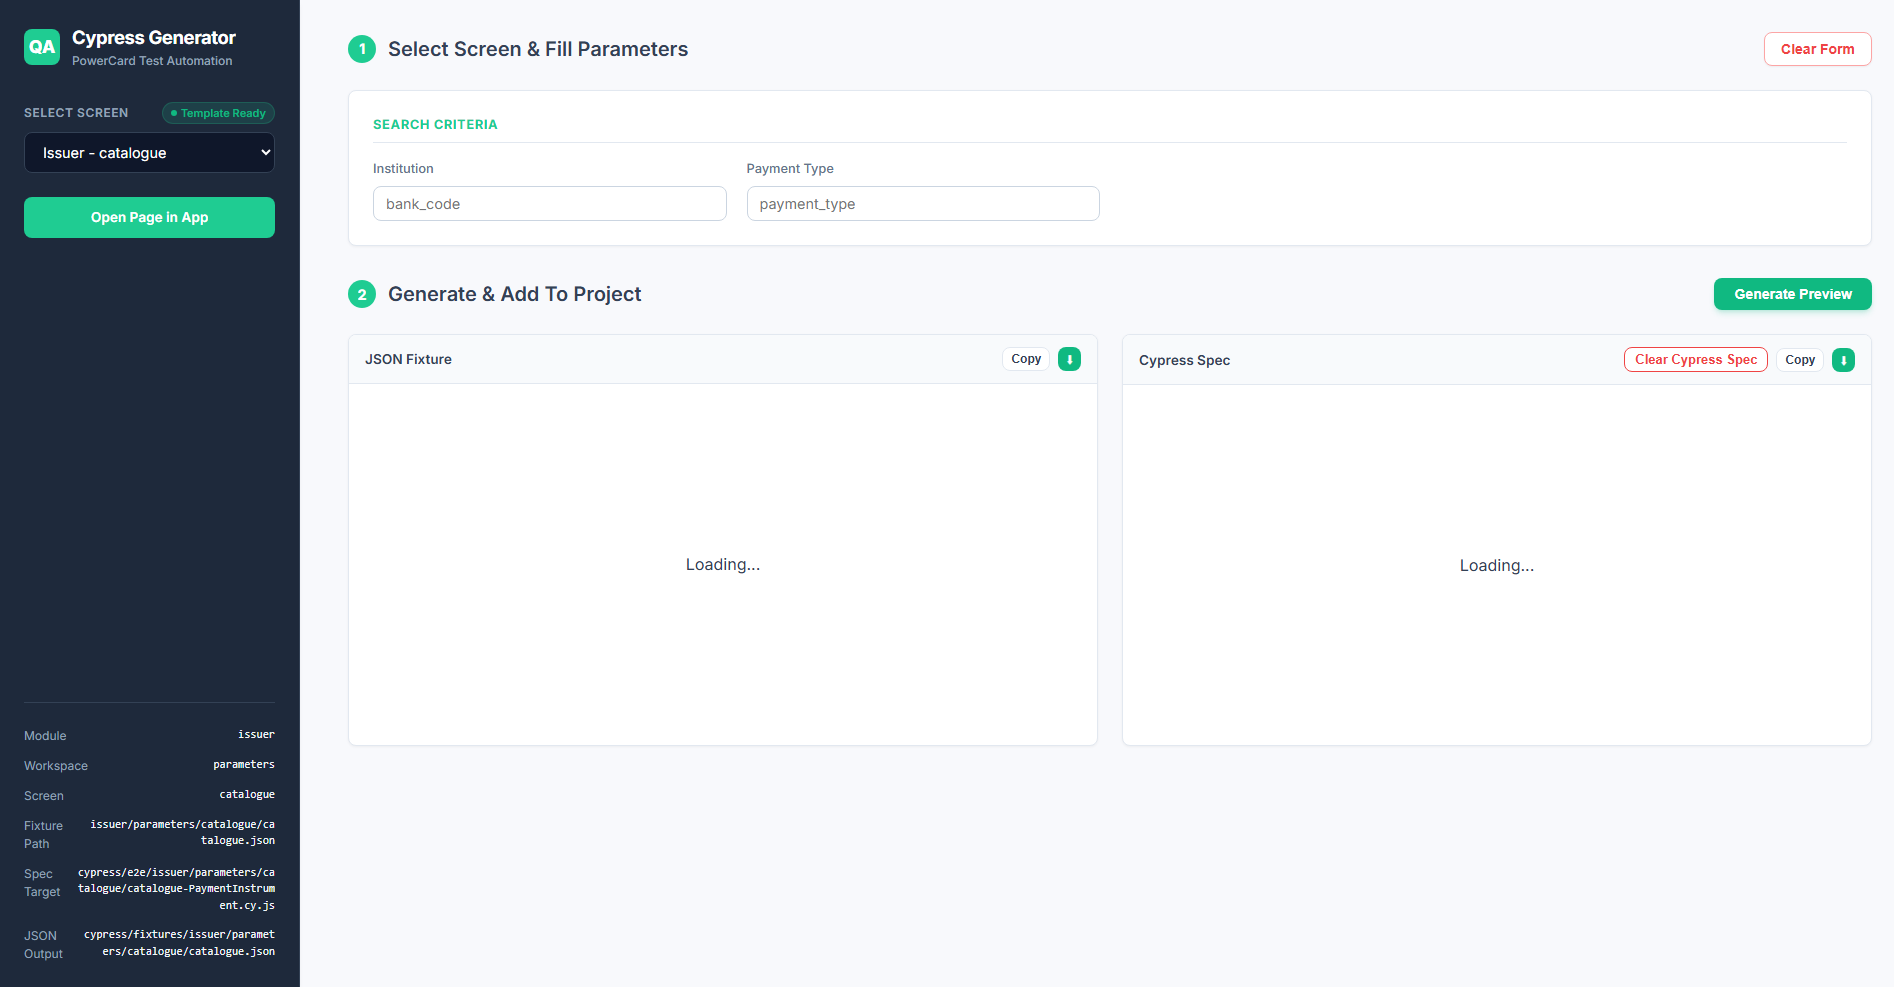
\includegraphics[width=\textwidth]{screenshots/chap-01.png}
\caption{Page d'accueil du Dashboard --- Vue globale de l'interface}
\end{figure}

L'interface d'accueil du Dashboard présente le menu latéral gauche (\textit{sidebar}) qui liste les 32 écrans PowerCARD catalogués, organisés par module (Switch, Issuer, Online, Acquiring). La zone centrale affiche les formulaires dynamiques et les éditeurs de code. Le design adopte un thème sombre professionnel avec des accents colorés pour la navigation.

\subsection{Étape 2 --- Sélection de l'écran MOTO}

\begin{figure}[H]
\centering
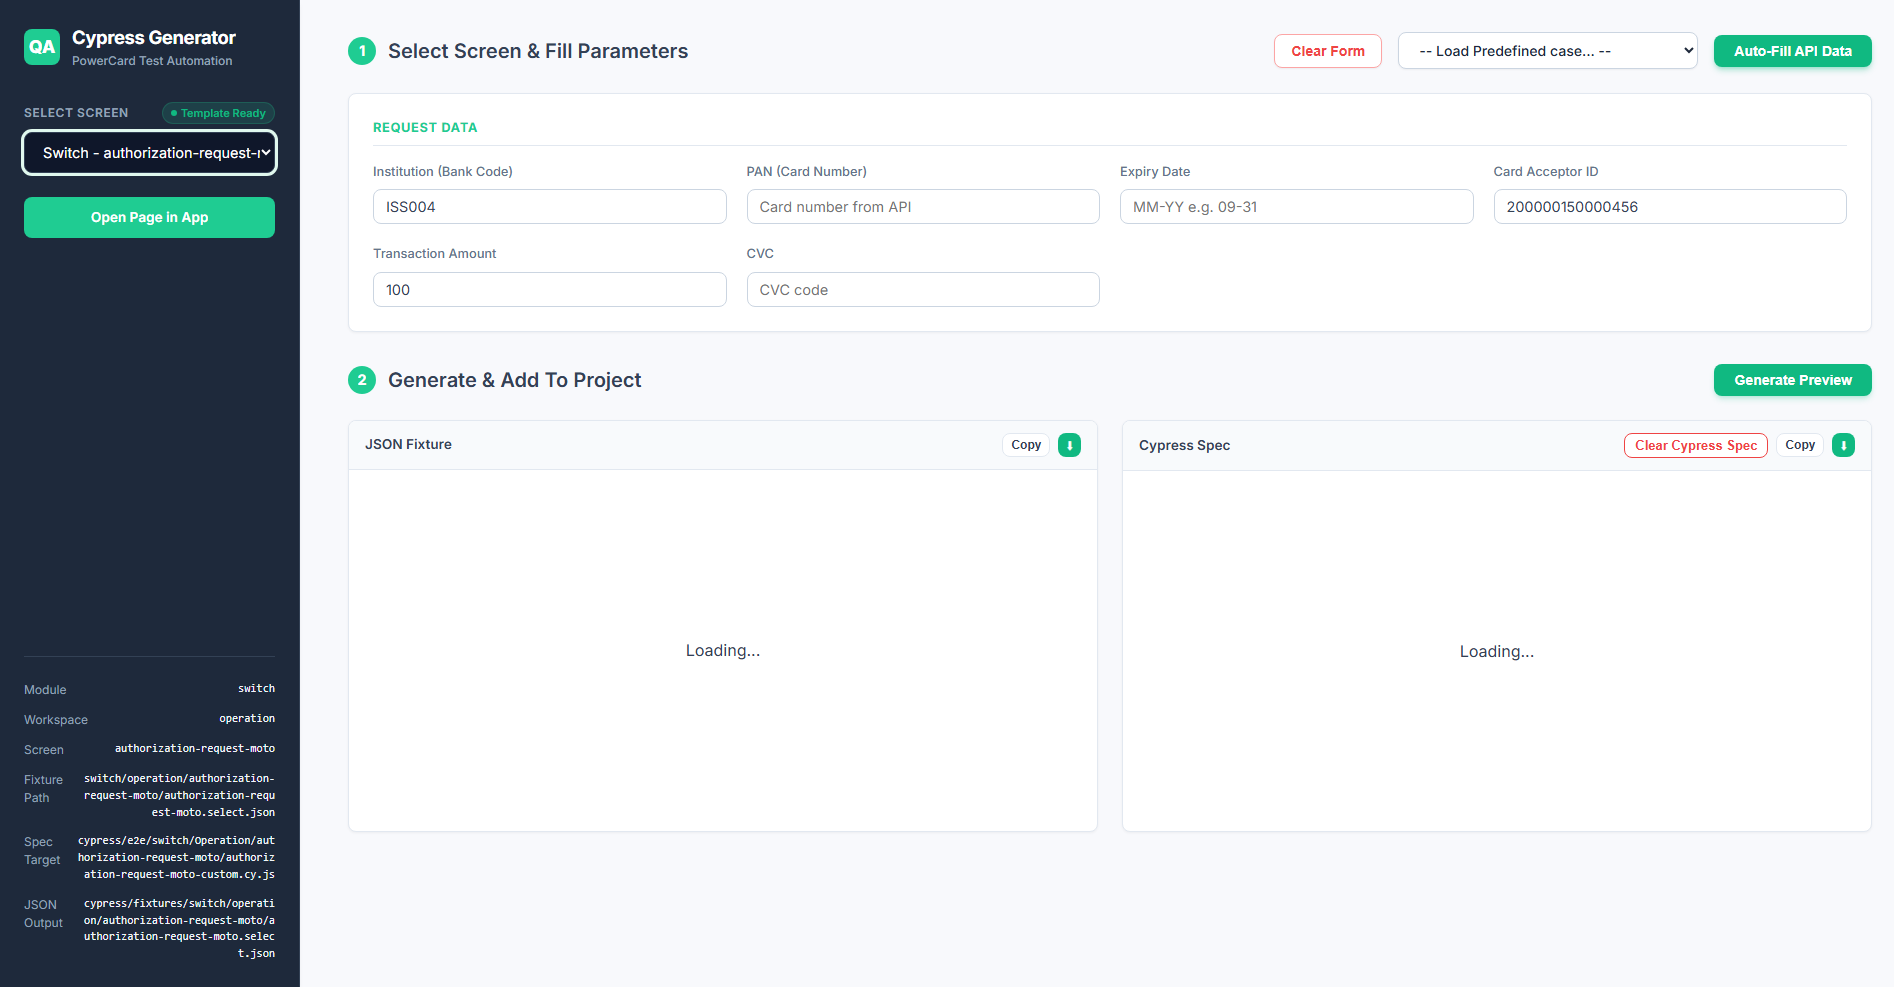
\includegraphics[width=\textwidth]{screenshots/chap-06.png}
\caption{Sélection de l'écran MOTO --- Le formulaire dynamique s'affiche automatiquement}
\end{figure}

En cliquant sur l'écran « Authorization Request MOTO » dans la sidebar, le Dashboard charge automatiquement le template de formulaire correspondant. Les champs affichés (Card Number, Expiry Date, Amount, Currency, etc.) sont spécifiques à ce type de transaction. Le système détecte le module (\texttt{switch}), le workspace (\texttt{operation}), et le chemin du spec Cypress associé.

\subsection{Étape 3 --- Auto-Fill API Data}

\begin{figure}[H]
\centering
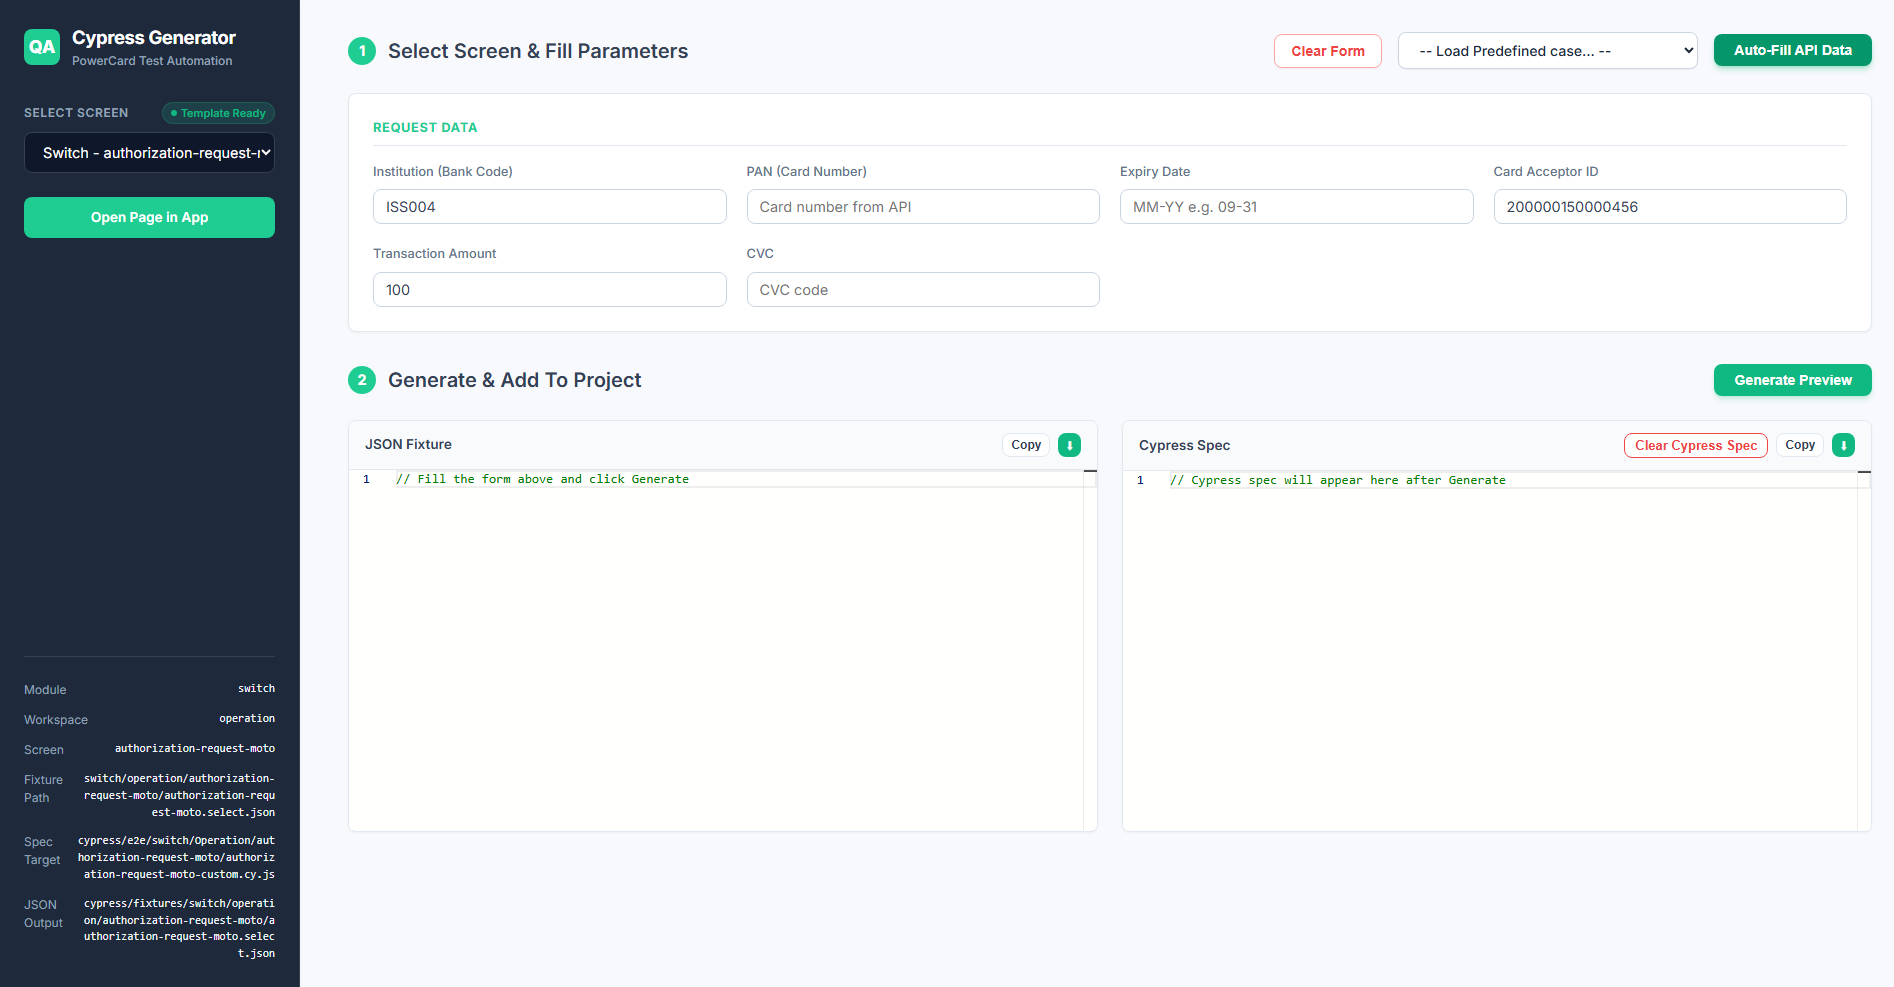
\includegraphics[width=\textwidth]{screenshots/chap-07.png}
\caption{Auto-Fill API Data --- Les données de carte sont récupérées automatiquement depuis l'API Connect}
\end{figure}

Le bouton « Auto-Fill API » déclenche un appel au proxy serveur qui s'authentifie auprès de l'API PowerCard Connect via JWT. Le système récupère automatiquement un numéro de carte de test valide, sa date d'expiration, et le code client associé. Ces données sont injectées dans les champs du formulaire, éliminant le besoin de saisie manuelle et garantissant la validité des données de test.

\subsection{Étape 4 --- Chargement d'un cas prédéfini}

\begin{figure}[H]
\centering
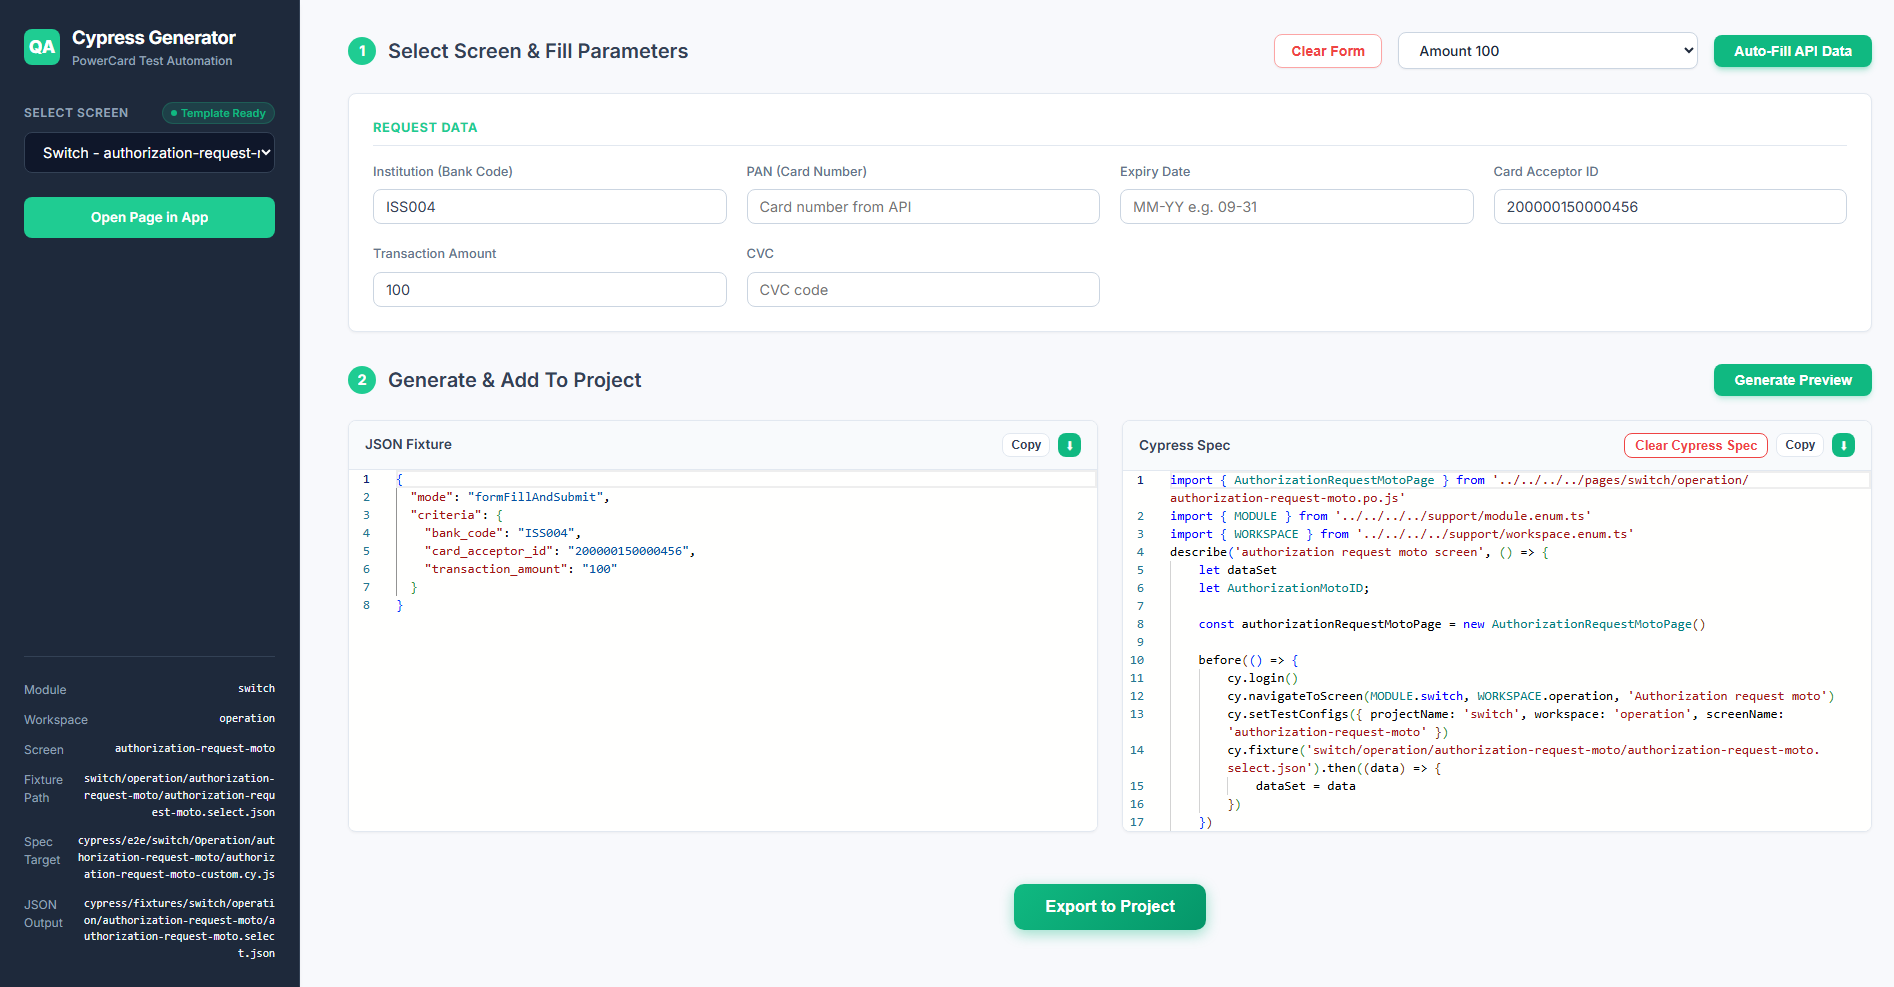
\includegraphics[width=\textwidth]{screenshots/chap-08.png}
\caption{Chargement d'un cas prédéfini --- Le montant de 100 est appliqué automatiquement}
\end{figure}

Le menu déroulant « Predefined Cases » permet de charger des jeux de données pré-configurés. Dans cet exemple, le cas « Amount 100 » remplit automatiquement le champ montant avec la valeur 100 et ajuste les autres paramètres de la transaction. Les cas prédéfinis sont définis dans \texttt{formTemplates.js} et permettent aux testeurs de reproduire rapidement des scénarios standards.

\subsection{Étape 5 --- Résultat de la génération}

\begin{figure}[H]
\centering
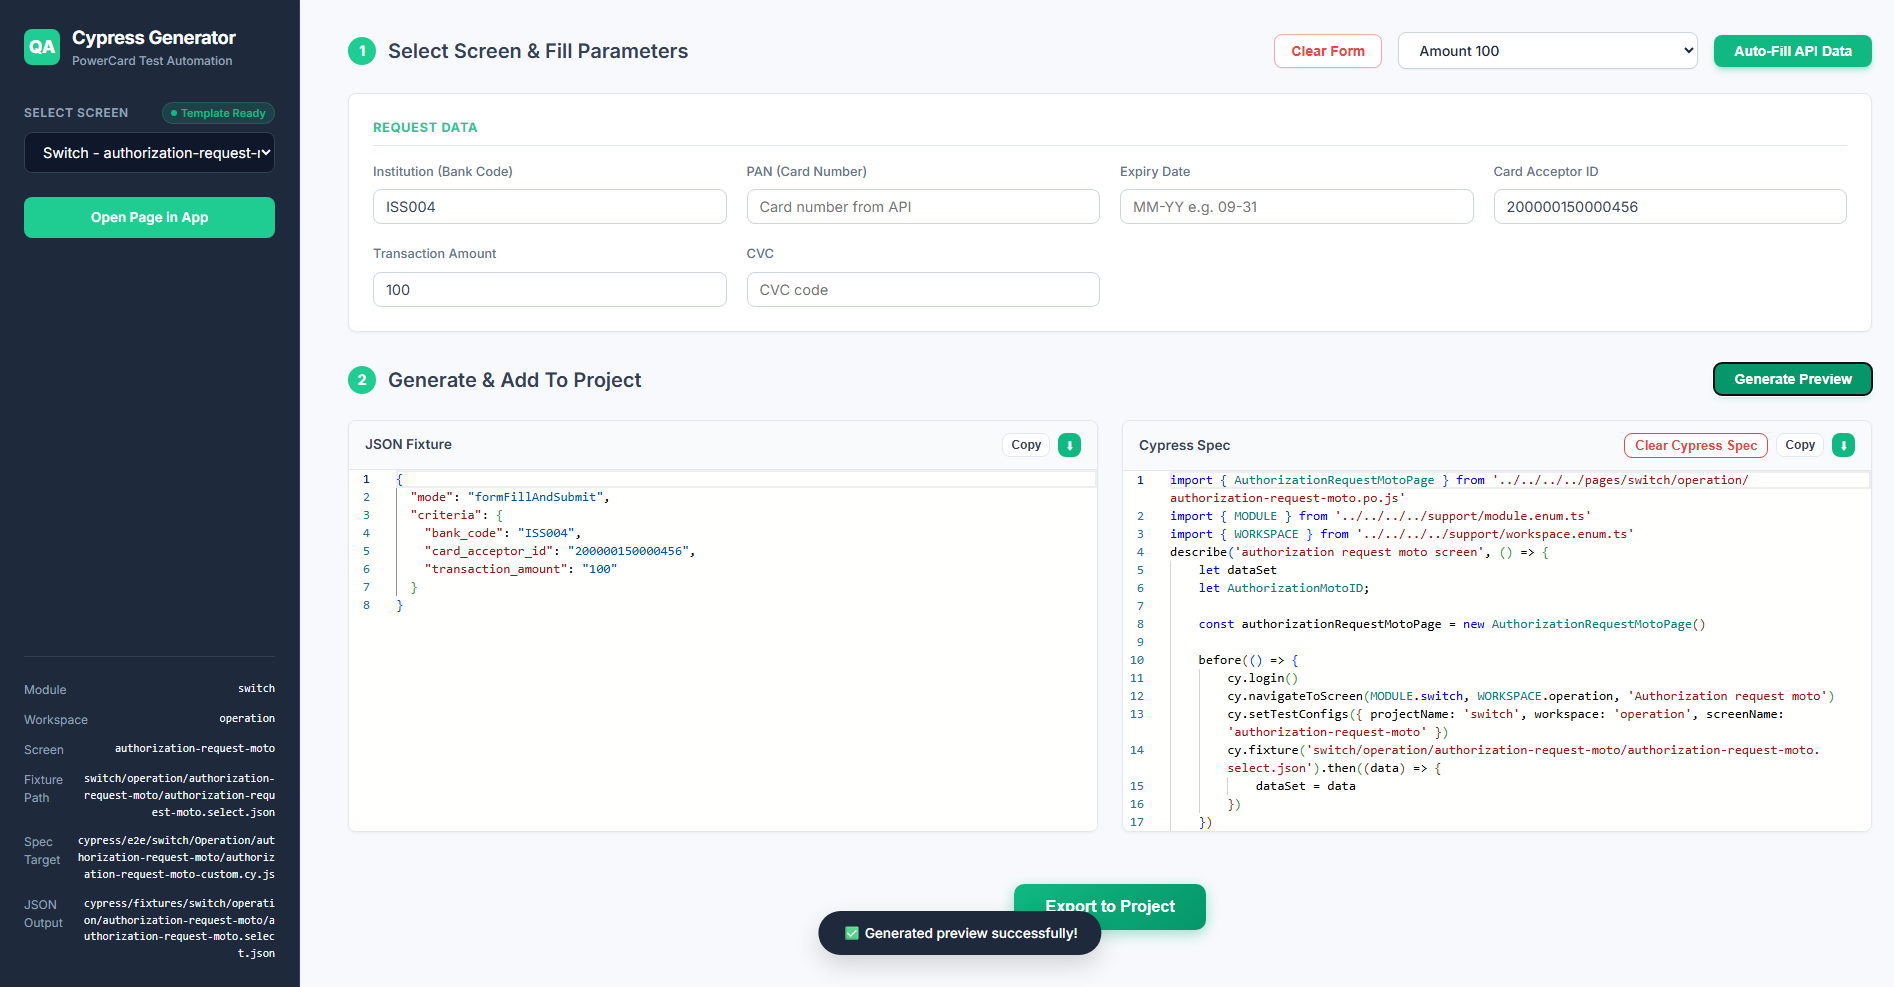
\includegraphics[width=\textwidth]{screenshots/chap-09.png}
\caption{Résultat de la génération --- Le JSON fixture et le Cypress Spec sont produits simultanément}
\end{figure}

Après avoir cliqué sur « Generate », le moteur de génération (\texttt{buildPayload()} + \texttt{patchSpec()}) produit simultanément deux fichiers : le \textbf{JSON fixture} contenant les données de test structurées, et le \textbf{Cypress Spec} (.cy.js) contenant le script de test complet. Les deux sont affichés côte à côte dans des éditeurs Monaco avec coloration syntaxique.

\subsection{Étape 6 --- Éditeurs Monaco}

\begin{figure}[H]
\centering
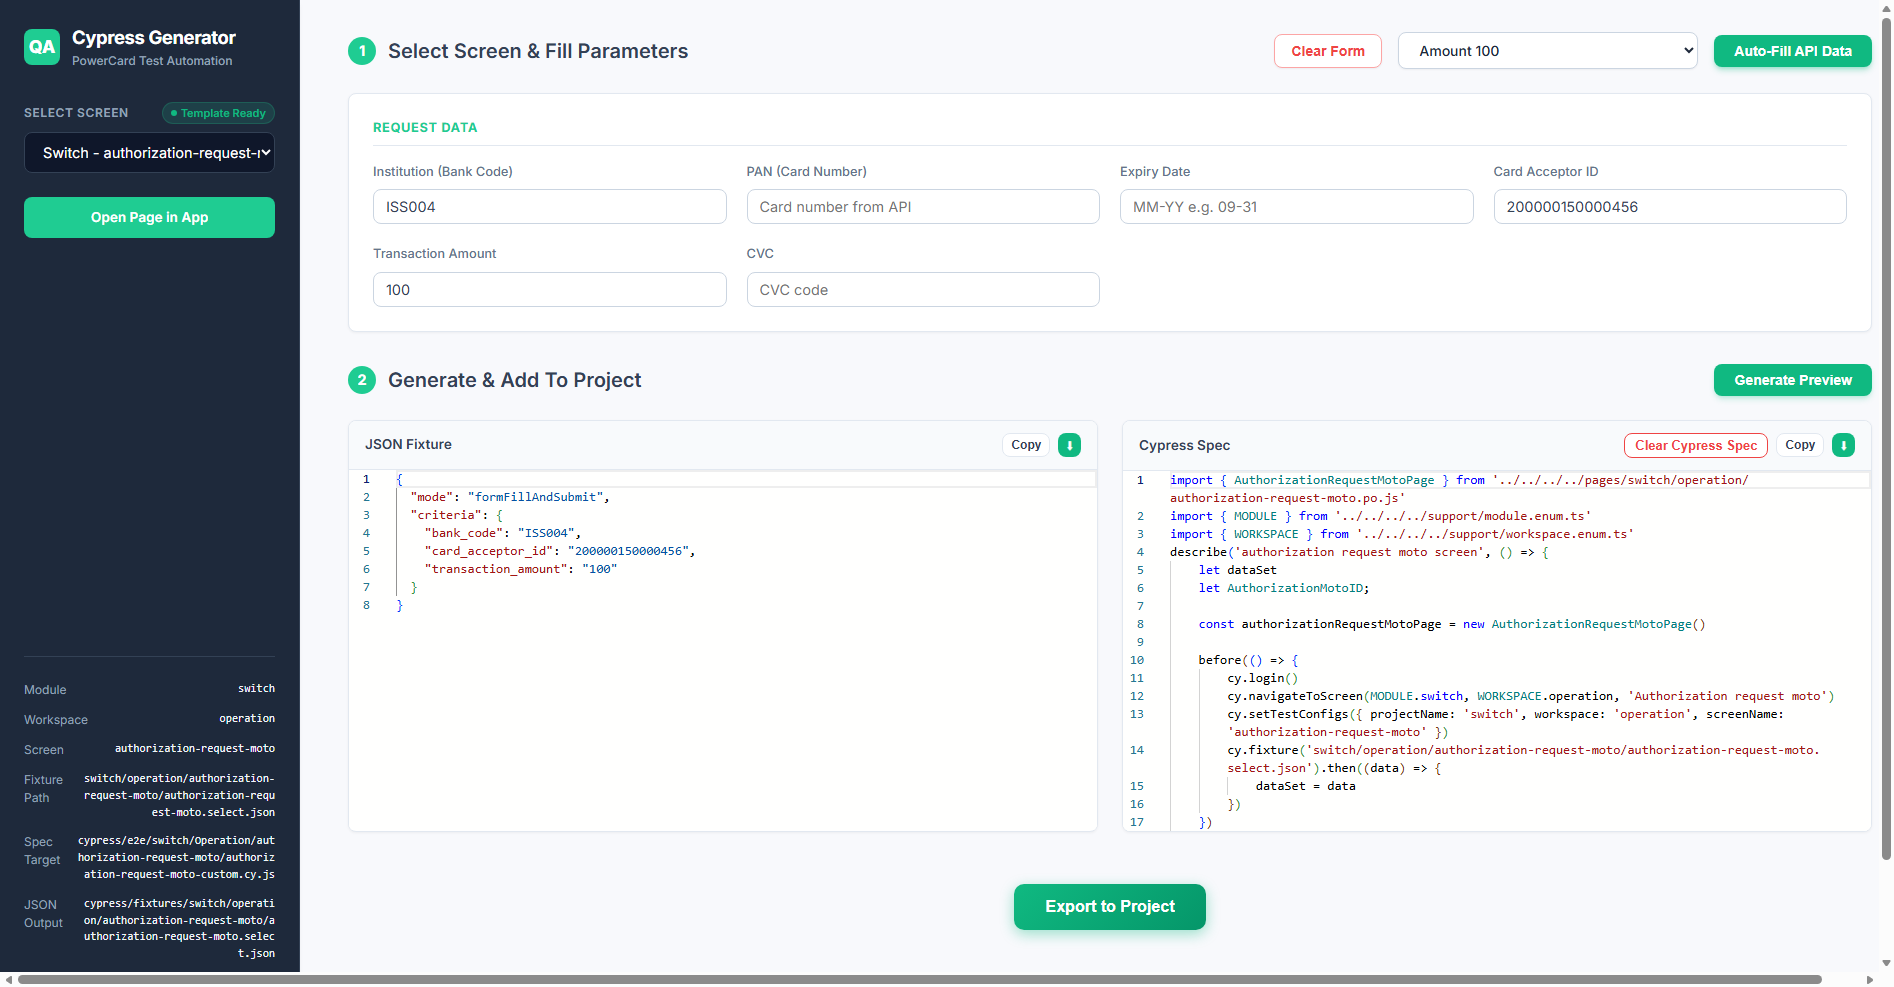
\includegraphics[width=\textwidth]{screenshots/chap-10.png}
\caption{Éditeurs Monaco --- Vue rapprochée avec coloration syntaxique JavaScript et JSON}
\end{figure}

Les éditeurs Monaco (le même moteur que VS Code) offrent une expérience de développement complète : coloration syntaxique, numérotation des lignes, pliage de code, et recherche. Le testeur peut vérifier et modifier le code généré avant de l'exporter. La partie gauche affiche le JSON fixture, la partie droite le script Cypress.

\subsection{Étape 7 --- Métadonnées dans la Sidebar}

\begin{figure}[H]
\centering
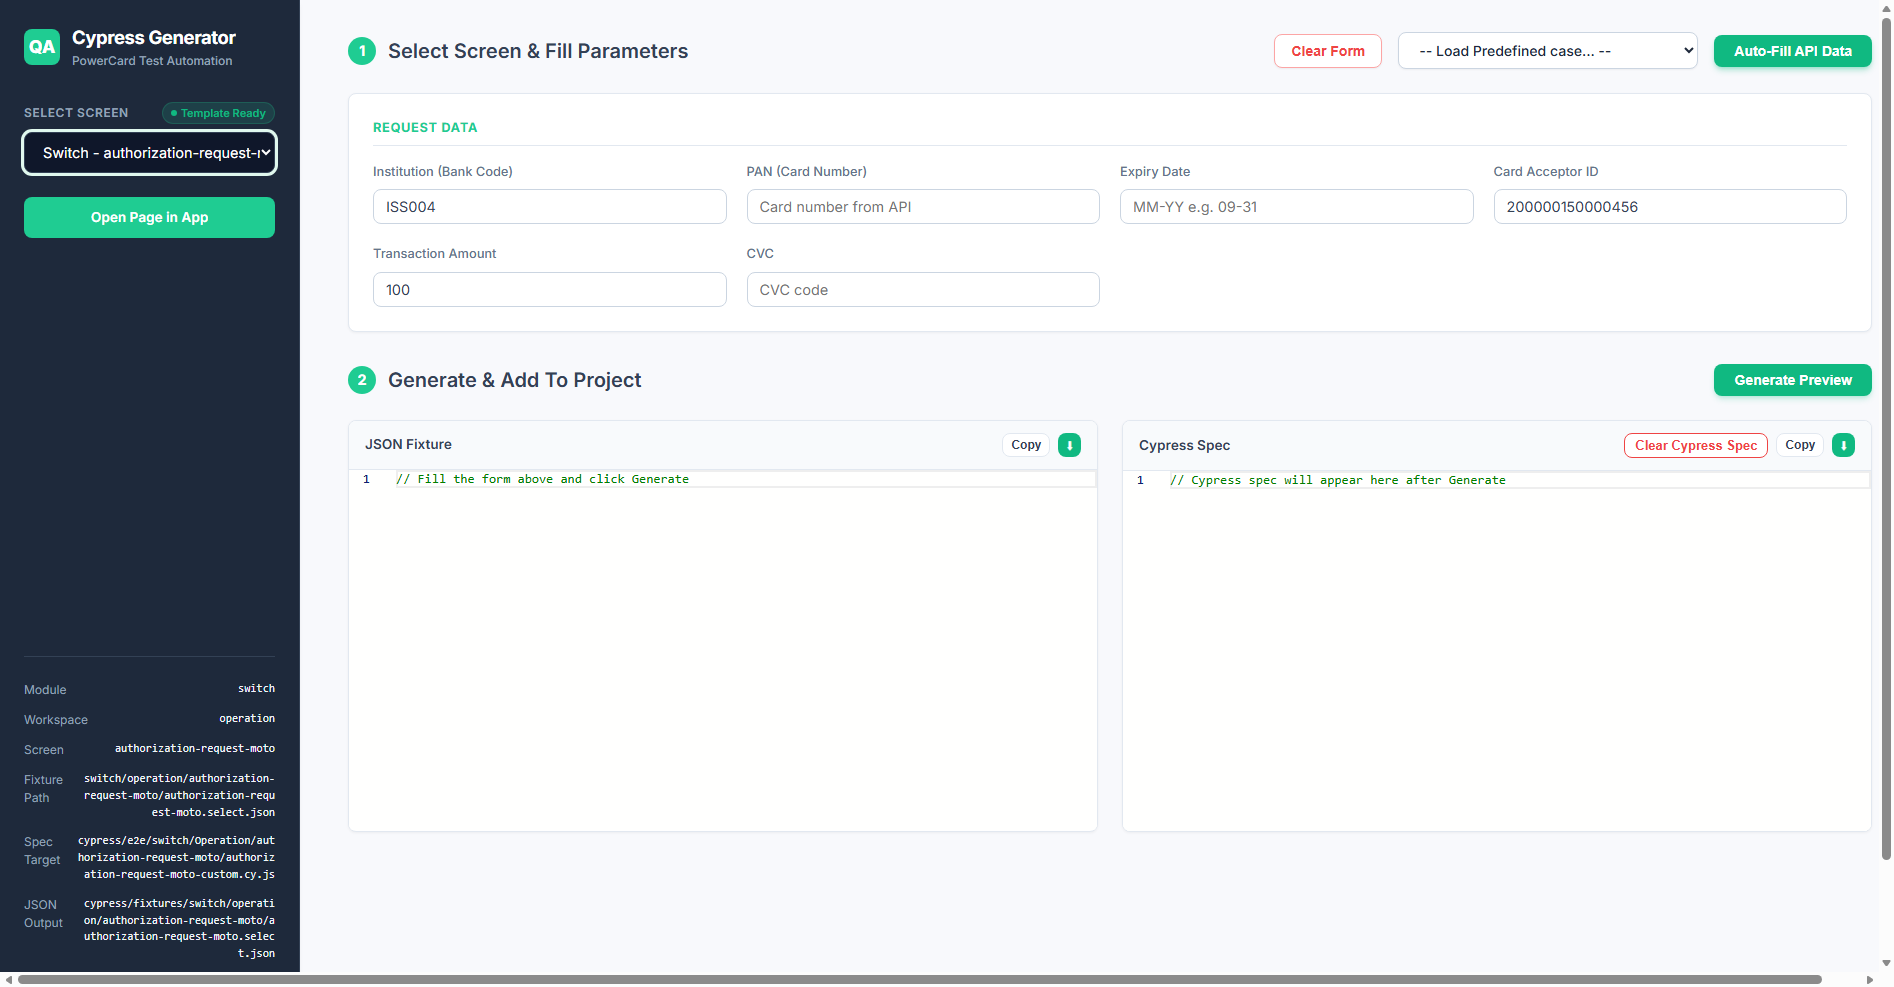
\includegraphics[width=\textwidth]{screenshots/chap-11.png}
\caption{Métadonnées de l'écran sélectionné --- Module, workspace, chemins des fichiers}
\end{figure}

La sidebar affiche les métadonnées complètes de l'écran sélectionné : le module (\texttt{switch}), le workspace (\texttt{operation}), le chemin du spec Cypress, le chemin du fixture JSON, et le nombre de champs du formulaire. Ces informations aident le testeur à comprendre l'organisation du projet et à localiser les fichiers générés.

\subsection{Étape 8 --- Module Issuer (autre exemple)}

\begin{figure}[H]
\centering
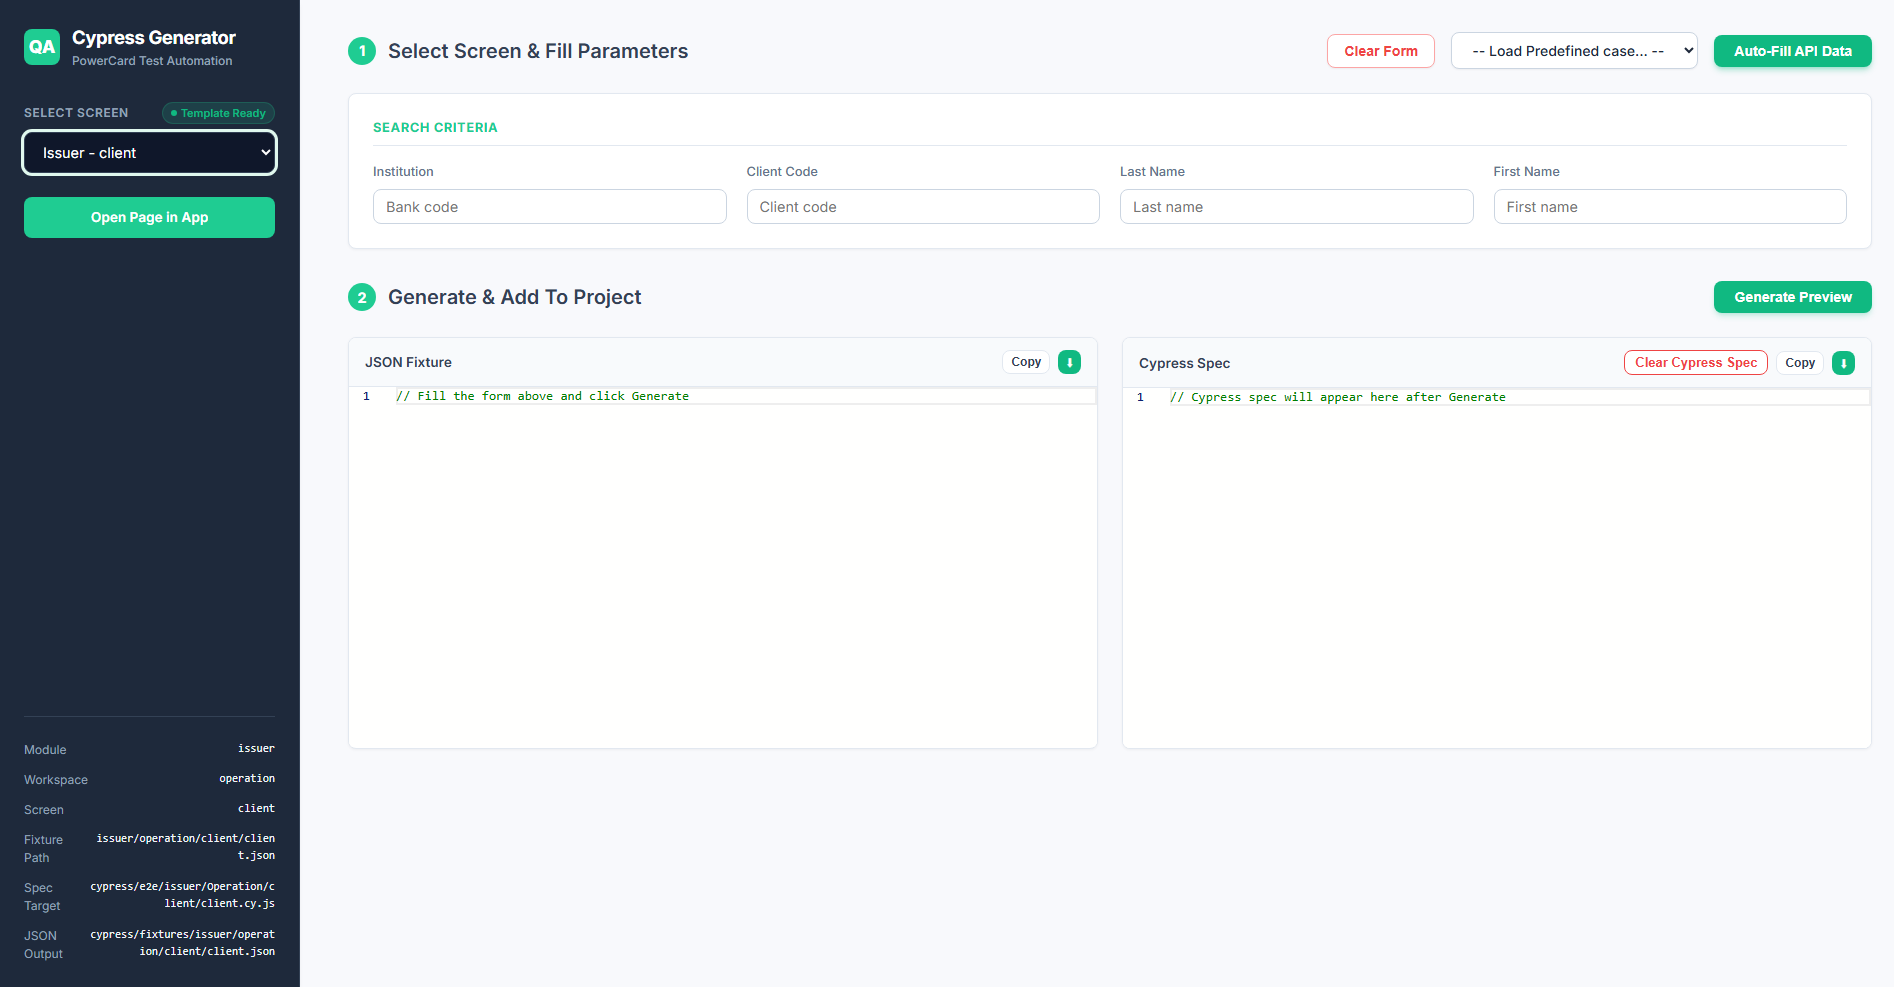
\includegraphics[width=\textwidth]{screenshots/chap-12.png}
\caption{Module Issuer --- L'écran Client avec ses champs spécifiques adaptés au contexte}
\end{figure}

Le Dashboard s'adapte dynamiquement au module sélectionné. Ici, l'écran « Client » du module Issuer affiche des champs différents de ceux du Switch MOTO : code institution, identifiant client, nom, adresse, etc. Cette flexibilité est rendue possible par le système de templates (\texttt{formTemplates.js}) qui mappe chaque écran à son formulaire spécifique.

\subsection{Étape 9 --- Export vers le projet}

\begin{figure}[H]
\centering
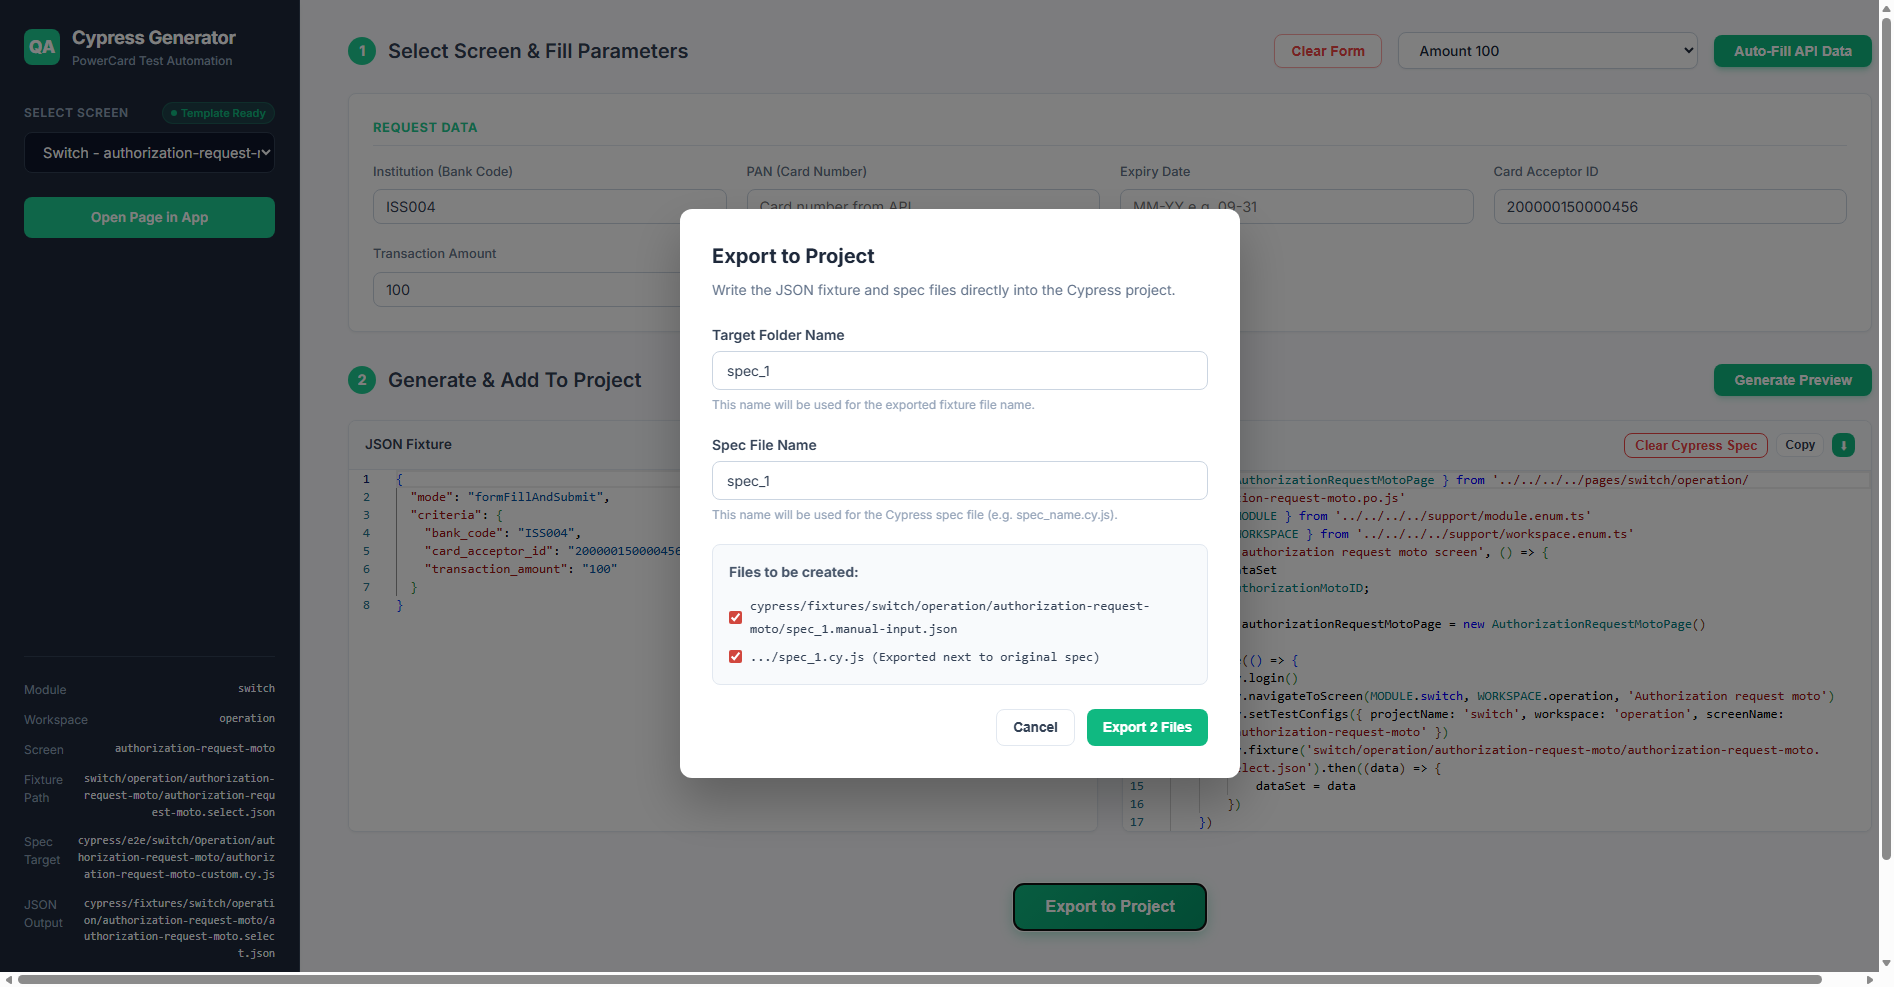
\includegraphics[width=\textwidth]{screenshots/chap-17-modal.png}
\caption{Modal d'export --- Confirmation avant écriture des fichiers dans l'arborescence Cypress}
\end{figure}

Le bouton « Export to Project » ouvre une modale de confirmation affichant les chemins exacts où les fichiers seront écrits : le fixture JSON dans \texttt{cypress/fixtures/} et le spec dans \texttt{cypress/e2e/}. Le serveur utilise \texttt{resolveSafeChildPath()} pour prévenir toute attaque de traversée de chemin avant d'écrire les fichiers via \texttt{fs.writeFileSync}.

\subsection{Étape 10 --- Exécution et rapport en temps réel}

\begin{figure}[H]
\centering
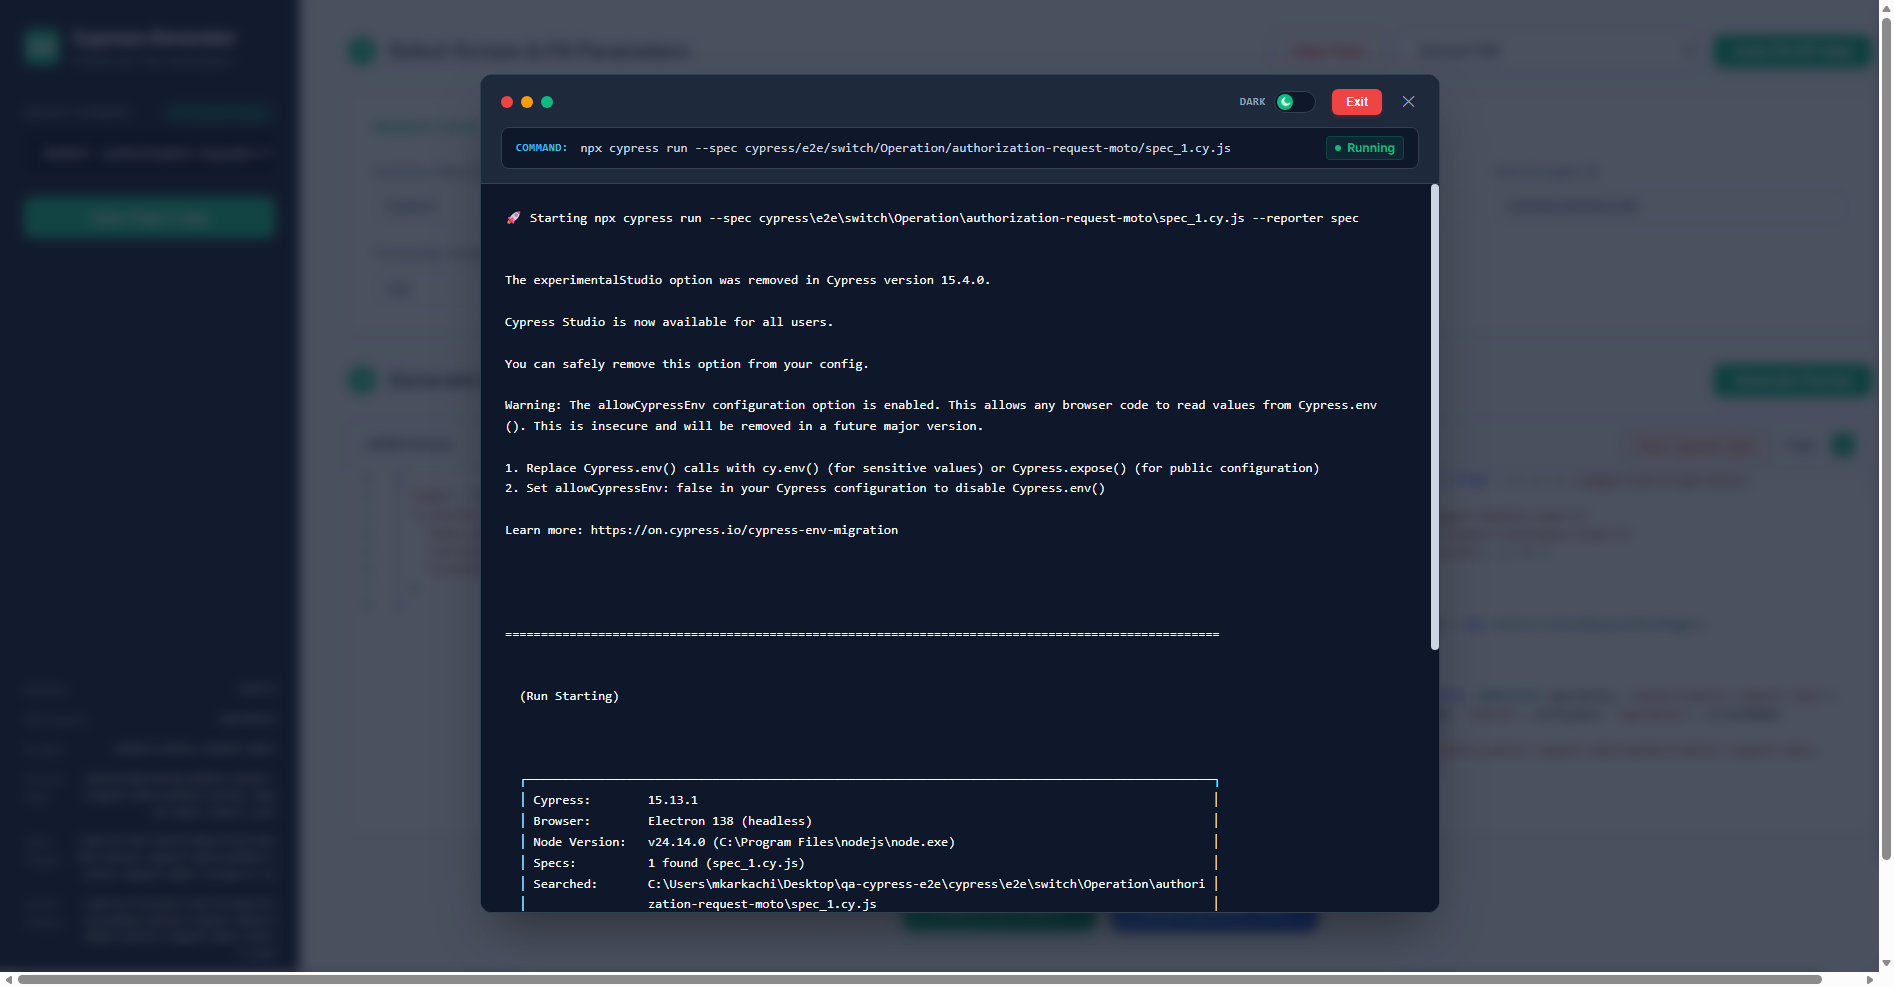
\includegraphics[width=\textwidth]{screenshots/chap-17-runner.png}
\caption{Terminal d'exécution intégré --- Les logs Cypress sont streamés en temps réel via SSE}
\end{figure}

Le terminal intégré dans le Dashboard affiche en temps réel les logs d'exécution du test Cypress. Le serveur Runner instancie un processus enfant (\texttt{spawn('npx cypress run --spec ...')}) et streame les sorties stdout/stderr via Server-Sent Events (SSE). Le parser \texttt{parseCypressLogs()} interprète les séquences d'échappement ANSI et colore les tests réussis en vert et les échecs en rouge.

\subsection{Étape 11 --- Résumé de l'exécution}

\begin{figure}[H]
\centering
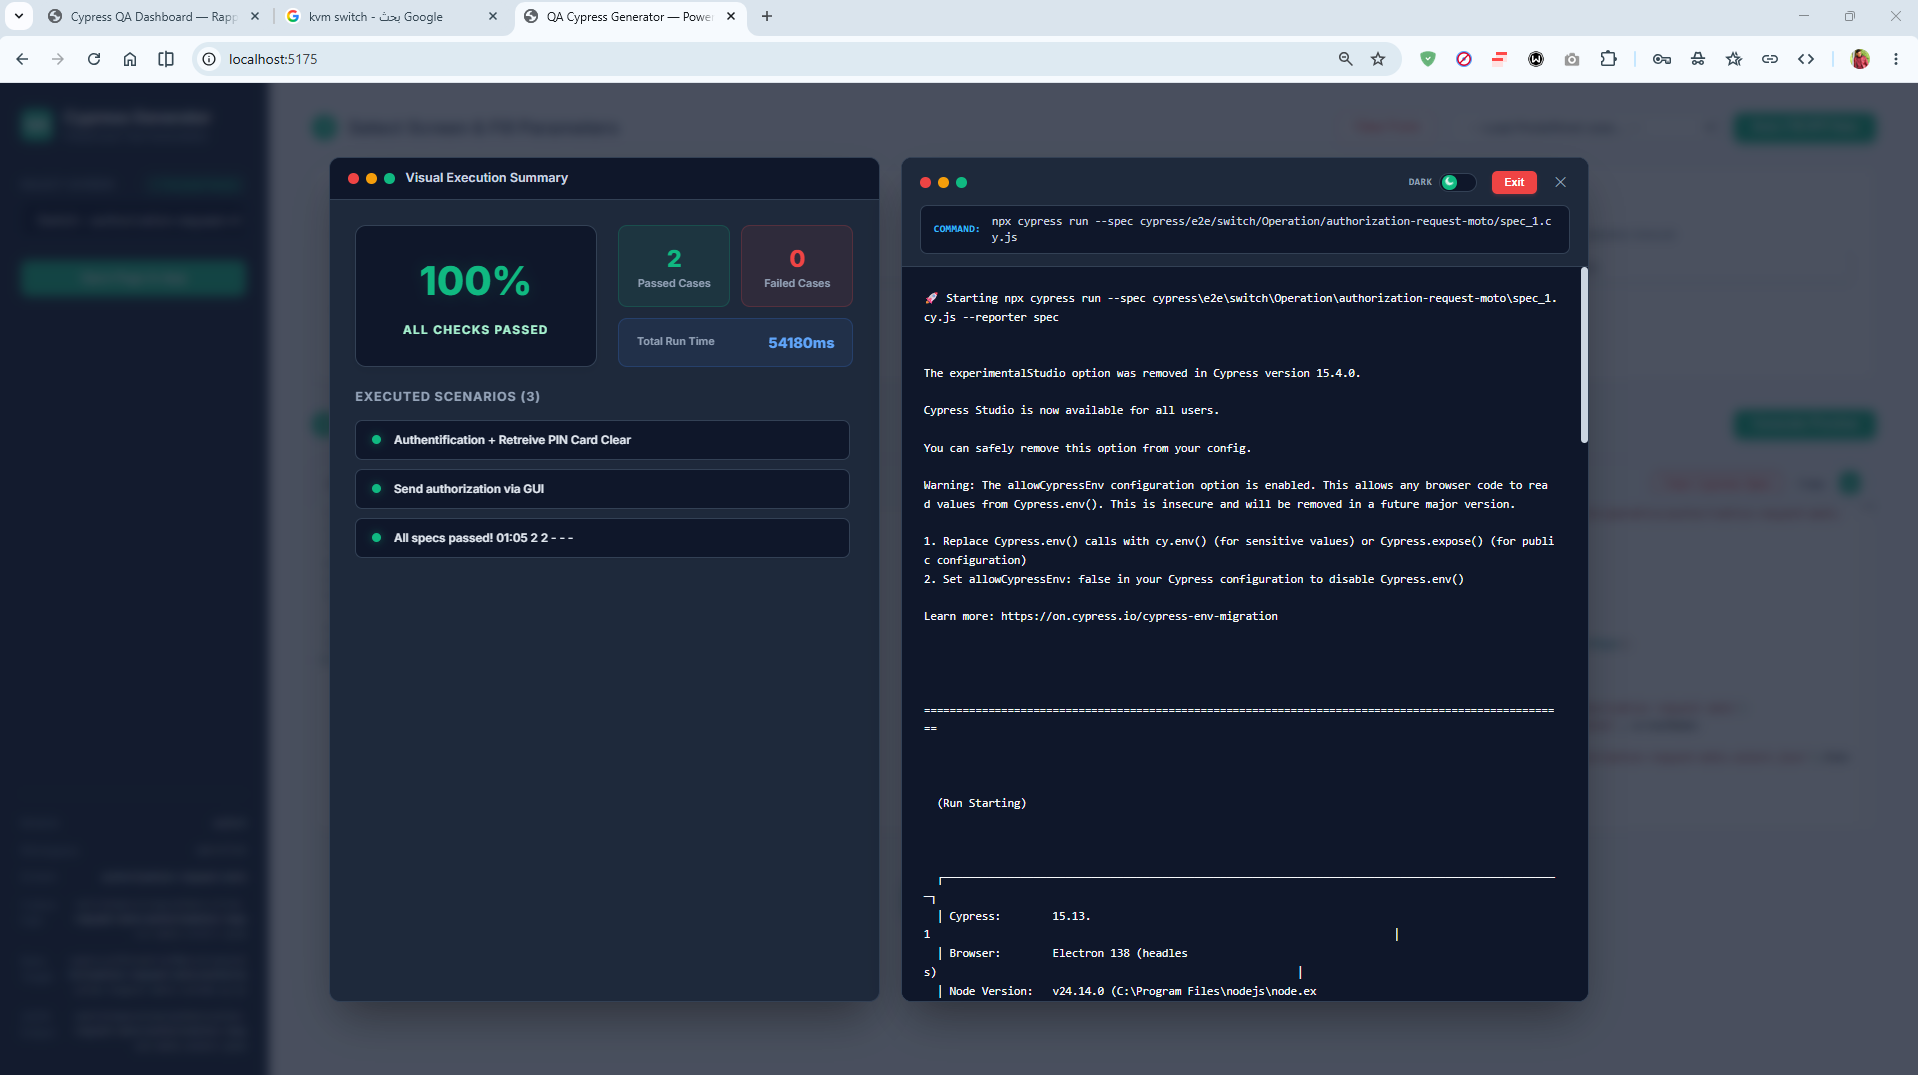
\includegraphics[width=\textwidth]{screenshots/chap-19-summary.png}
\caption{Résumé de l'exécution --- Pourcentage de succès, nombre de tests, et temps total}
\end{figure}

À la fin de l'exécution, le Dashboard affiche un résumé structuré : le pourcentage de réussite, le nombre de tests passés/échoués, et le temps total d'exécution. Cette vue synthétique permet aux testeurs de rapidement évaluer la qualité du module testé sans avoir à analyser les logs bruts.


% ══════════════════════════════════════════════════════════════════
% SECTION 3: RAPPORT QA --- CYCLE DE VIE DU TERMINAL
% ══════════════════════════════════════════════════════════════════
\newpage
\section{Rapport QA --- Cycle de vie du Terminal}

\textit{Cette section présente le rapport d'automatisation QA pour le scénario de test du Cycle de vie du Terminal, couvrant les fonctionnalités Network MCC Mapping et Merchant Onboarding sur PowerCARD V4.3.1-develop.}

\vspace{10pt}


\begin{tcolorbox}[colback=primary!5, colframe=primary, title=Aperçu du Projet \& Constats Critiques, arc=5pt]
    \begin{itemize}[leftmargin=1.5em]
        \item \textbf{Sujet :} Validation du Mapping Network MCC
        \item \textbf{Environnement :} Espaces de travail Administration \& Opération (V4.3.1-develop)
        \item \textbf{Statut d'exécution :} \textcolor{success}{8 Réussis}, \textcolor{warning}{0 Ignorés}, \textcolor{danger}{2 Échoués (Défauts)}
        \item \textbf{Date :} 2026-05-12
    \end{itemize}
    
    \vspace{0.3cm}
    \textbf{\large Résumé des bugs principaux (Journal Jira) :}
    \begin{itemize}[leftmargin=1.5em, itemsep=3pt]
        \item \textbf{BF-911 (Défaut) :} Les données ne sont pas conservées dans le champ obligatoire « Ville » après la confirmation de l'enregistrement.
        \item \textbf{BF-912 (Défaut) :} Interface - L'indicateur d'onglet dans la navigation latérale reste vert lorsqu'un champ obligatoire est en état d'erreur.
        \item \textbf{BF-916 (Défaut/Processus) :} [Network Mcc Mapping] Améliorations de la validation du tableau et du flux de travail.
        \item \textbf{BF-921 (Défaut Critique) :} [Network Mcc Mapping] L'enregistrement échoue avec une fenêtre d'erreur lorsque tous les champs sont remplis.
    \end{itemize}
\end{tcolorbox}

\subsection{Résumé de l'Exécution des Tests}

\begin{tcolorbox}[colback=primary!5, colframe=primary, title=\textbf{Résumé Exécutif}]
Ce cycle de test s'est concentré sur la fonctionnalité de \textbf{Mapping Network MCC du Marchand}. Sur 10 scénarios testés, 8 ont réussi, confirmant que la configuration de base et la navigation fonctionnent comme prévu. Cependant, un \textbf{problème bloquant critique} a été identifié lors de l'enregistrement d'une grille complète de mappings.
\end{tcolorbox}

\begin{center}
\renewcommand{\arraystretch}{1.5}
\begin{tabular}{|c|c|c|c|}
\hline
\textbf{Total CT} & \cellcolor{successbg}\textcolor{white}{\textbf{Réussis}} & \cellcolor{warningbg}\textcolor{white}{\textbf{Ignorés}} & \cellcolor{dangerbg}\textcolor{white}{\textbf{Échoués}} \\
\hline
\textbf{10} & \textcolor{successbg}{\textbf{8}} & \textcolor{warningbg}{\textbf{0}} & \textcolor{dangerbg}{\textbf{2}} \\
\hline
\end{tabular}
\end{center}

\subsection{Mapping Network MCC (\texttt{network-mcc-mapping.cy.js})}

\vspace{0.3cm}
\noindent
\begin{minipage}{\textwidth}
\renewcommand{\arraystretch}{1.5}
\begin{tabular}{|p{3cm}|p{12.5cm}|}
\hline
\rowcolor{primary}
\textcolor{white}{\textbf{Section}} & \textcolor{white}{\textbf{Détails}} \\
\hline
\multicolumn{2}{|c|}{\cellcolor{gray!20}\textbf{OPÉRATION DE LECTURE}} \\
\hline
\textbf{Bloc it()} & \texttt{it('READ: Verify screen and search MCC')} \\
\hline
\textbf{Actions} & $\bullet$ Vérifier les éléments de l'écran (champs MCC, bouton Ajouter).\newline $\bullet$ Rechercher en utilisant le code MCC 3847. \\
\hline
\textbf{Statut} & \textcolor{success}{\textbf{RÉUSSI}} \\
\hline
\end{tabular}
\end{minipage}

\vspace{0.5cm}
\noindent
\begin{minipage}{\textwidth}
\renewcommand{\arraystretch}{1.5}
\begin{tabular}{|p{3cm}|p{12.5cm}|}
\hline
\rowcolor{primary}
\textcolor{white}{\textbf{Section}} & \textcolor{white}{\textbf{Détails}} \\
\hline
\multicolumn{2}{|c|}{\cellcolor{gray!20}\textbf{OPÉRATION DE CRÉATION}} \\
\hline
\textbf{Bloc it()} & \texttt{it('CREATE: Add all networks, save and verify success')} \\
\hline
\textbf{Actions} & $\bullet$ Ajouter la première ligne (UPI) avec le MCC 7011.\newline $\bullet$ Ajouter récursivement tous les réseaux restants.\newline $\bullet$ Cliquer sur le bouton Enregistrer. \\
\hline
\textbf{Statut} & \textcolor{danger}{\textbf{ÉCHOUÉ}} (Défaut Critique \textbf{BF-921} - 500 Erreur interne) \\
\hline
\end{tabular}
\end{minipage}

\vspace{0.5cm}
\noindent
\begin{minipage}{\textwidth}
\renewcommand{\arraystretch}{1.5}
\begin{tabular}{|p{3cm}|p{12.5cm}|}
\hline
\rowcolor{primary}
\textcolor{white}{\textbf{Section}} & \textcolor{white}{\textbf{Détails}} \\
\hline
\multicolumn{2}{|c|}{\cellcolor{gray!20}\textbf{OPÉRATION DE MISE À JOUR}} \\
\hline
\textbf{Bloc it()} & \texttt{it('UPDATE: Modify MCC value, save and verify success')} \\
\hline
\textbf{Actions} & $\bullet$ Mettre à jour le code MCC de la première ligne (8888).\newline $\bullet$ Cliquer sur Enregistrer. \\
\hline
\textbf{Statut} & \textcolor{success}{\textbf{RÉUSSI}} \\
\hline
\end{tabular}
\end{minipage}

\vspace{0.5cm}
\noindent
\begin{minipage}{\textwidth}
\renewcommand{\arraystretch}{1.5}
\begin{tabular}{|p{3cm}|p{12.5cm}|}
\hline
\rowcolor{primary}
\textcolor{white}{\textbf{Section}} & \textcolor{white}{\textbf{Détails}} \\
\hline
\multicolumn{2}{|c|}{\cellcolor{gray!20}\textbf{OPÉRATION DE SUPPRESSION}} \\
\hline
\textbf{Bloc it()} & \texttt{it('DELETE: Remove a single row and verify')} \\
\hline
\textbf{Actions} & $\bullet$ Cliquer sur supprimer sur une ligne spécifique et confirmer. \\
\hline
\textbf{Statut} & \textcolor{success}{\textbf{RÉUSSI}} \\
\hline
\end{tabular}
\end{minipage}


\subsection{Merchant Onboarding (\texttt{merchant-onboarding.cy.js})}

\vspace{0.3cm}
\noindent
\begin{minipage}{\textwidth}
\renewcommand{\arraystretch}{1.5}
\begin{tabular}{|p{3cm}|p{12.5cm}|}
\hline
\rowcolor{primary}
\textcolor{white}{\textbf{Section}} & \textcolor{white}{\textbf{Détails}} \\
\hline
\multicolumn{2}{|c|}{\cellcolor{gray!20}\textbf{CRÉATION DU MARCHAND}} \\
\hline
\textbf{Bloc it()} & \texttt{it('CREATE: Fill all tabs and save Merchant')} \\
\hline
\textbf{Actions} & $\bullet$ Cliquer sur Nouveau.\newline $\bullet$ Remplir les onglets Description, Statut, Localisation.\newline $\bullet$ Cliquer sur Enregistrer. \\
\hline
\textbf{Statut} & \textcolor{success}{\textbf{RÉUSSI}} \\
\hline
\end{tabular}
\end{minipage}

\vspace{0.5cm}
\noindent
\begin{minipage}{\textwidth}
\renewcommand{\arraystretch}{1.5}
\begin{tabular}{|p{3cm}|p{12.5cm}|}
\hline
\rowcolor{primary}
\textcolor{white}{\textbf{Section}} & \textcolor{white}{\textbf{Détails}} \\
\hline
\multicolumn{2}{|c|}{\cellcolor{gray!20}\textbf{VÉRIFICATION PERSISTANCE}} \\
\hline
\textbf{Bloc it()} & \texttt{it('UPDATE: Open merchant, check City field')} \\
\hline
\textbf{Actions} & $\bullet$ Double-cliquer pour ouvrir les détails.\newline $\bullet$ Naviguer vers l'onglet Localisation.\newline $\bullet$ Vérifier si la valeur du champ Ville est conservée. \\
\hline
\textbf{Statut} & \textcolor{danger}{\textbf{ÉCHOUÉ}} (\textbf{BF-911} - Données non conservées dans le champ Ville) \\
\hline
\end{tabular}
\end{minipage}


% ── Étapes de Test avec Captures ──
\newpage
\subsection{Étapes de Test --- Captures d'écran}

\subsubsection{Connexion à PowerCARD}

\twoimages{login_empty.png}{Connexion PowerCARD --- Formulaire vide}
          {login_filled.png}{Connexion PowerCARD --- Identifiants remplis (ISS007)}

\begin{lstlisting}[caption={Code de connexion}]
cy.clearCookies()
cy.clearLocalStorage()
cy.login('ISS007', '*********')
cy.waitBusy()
\end{lstlisting}

\subsubsection{Navigation vers le Mapping Network MCC}

\twoimages{search_mcc.png}{Rechercher ``Network MCC mapping''}
          {empty_mcc.png}{Mapping Network MCC --- Formulaire vide}

\subsubsection{Saisie du Code MCC et Tests Négatifs}

\twoimages{loaded_mcc.png}{MCC 3847 chargé avec les données d'institution}
          {tc8.png}{Validation : Erreur de clé étrangère (test négatif)}

\subsubsection{Ajout des Mappings et Enregistrement}

\begin{figure}[H]
    \centering
    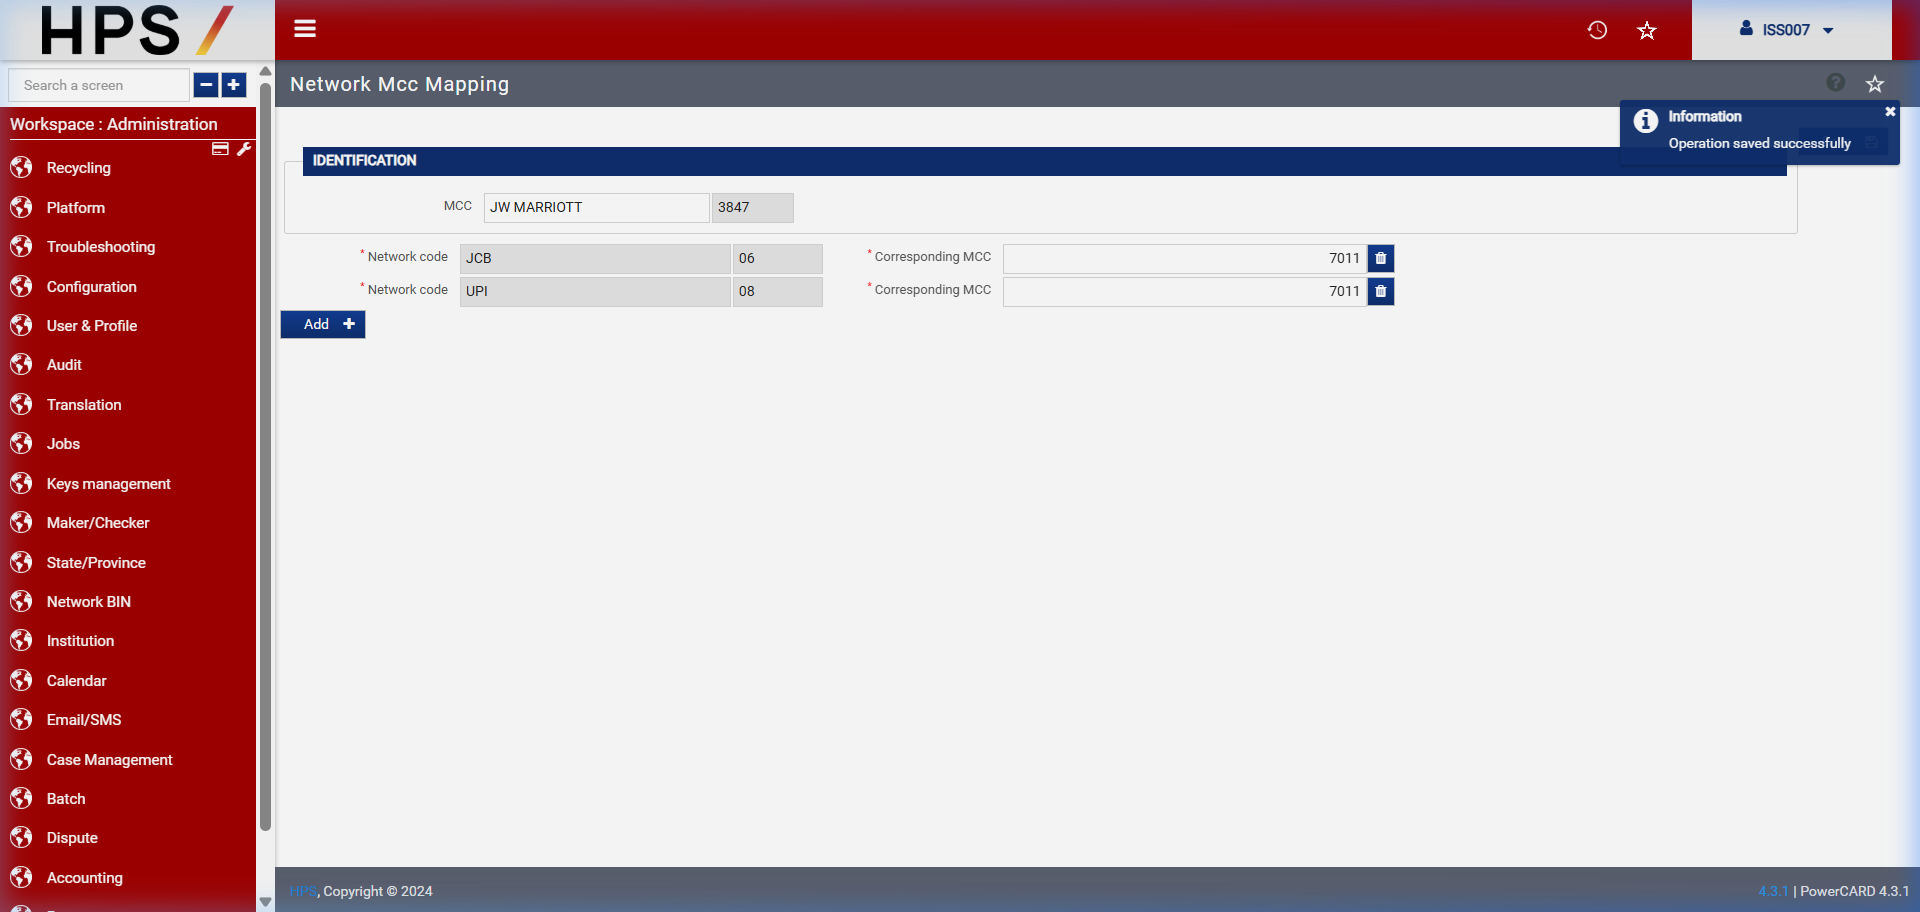
\includegraphics[width=0.8\textwidth]{save_success.png}
    \caption{Opération enregistrée avec succès}
\end{figure}

\subsubsection{Intégration du Marchand (Espace Opération)}

\twoimages{op_dashboard.png}{Tableau de bord Opération}
          {pos_module.png}{Barre latérale du module Pos}

\twoimages{step12_empty.png}{Formulaire de marchand vide}
          {step13_desc.png}{Onglet Description rempli}

\twoimages{step14_loc.png}{Onglet Localisation}
          {step15_success.png}{Opération enregistrée avec succès}

\subsubsection{Vérification Finale}

\begin{figure}[H]
    \centering
    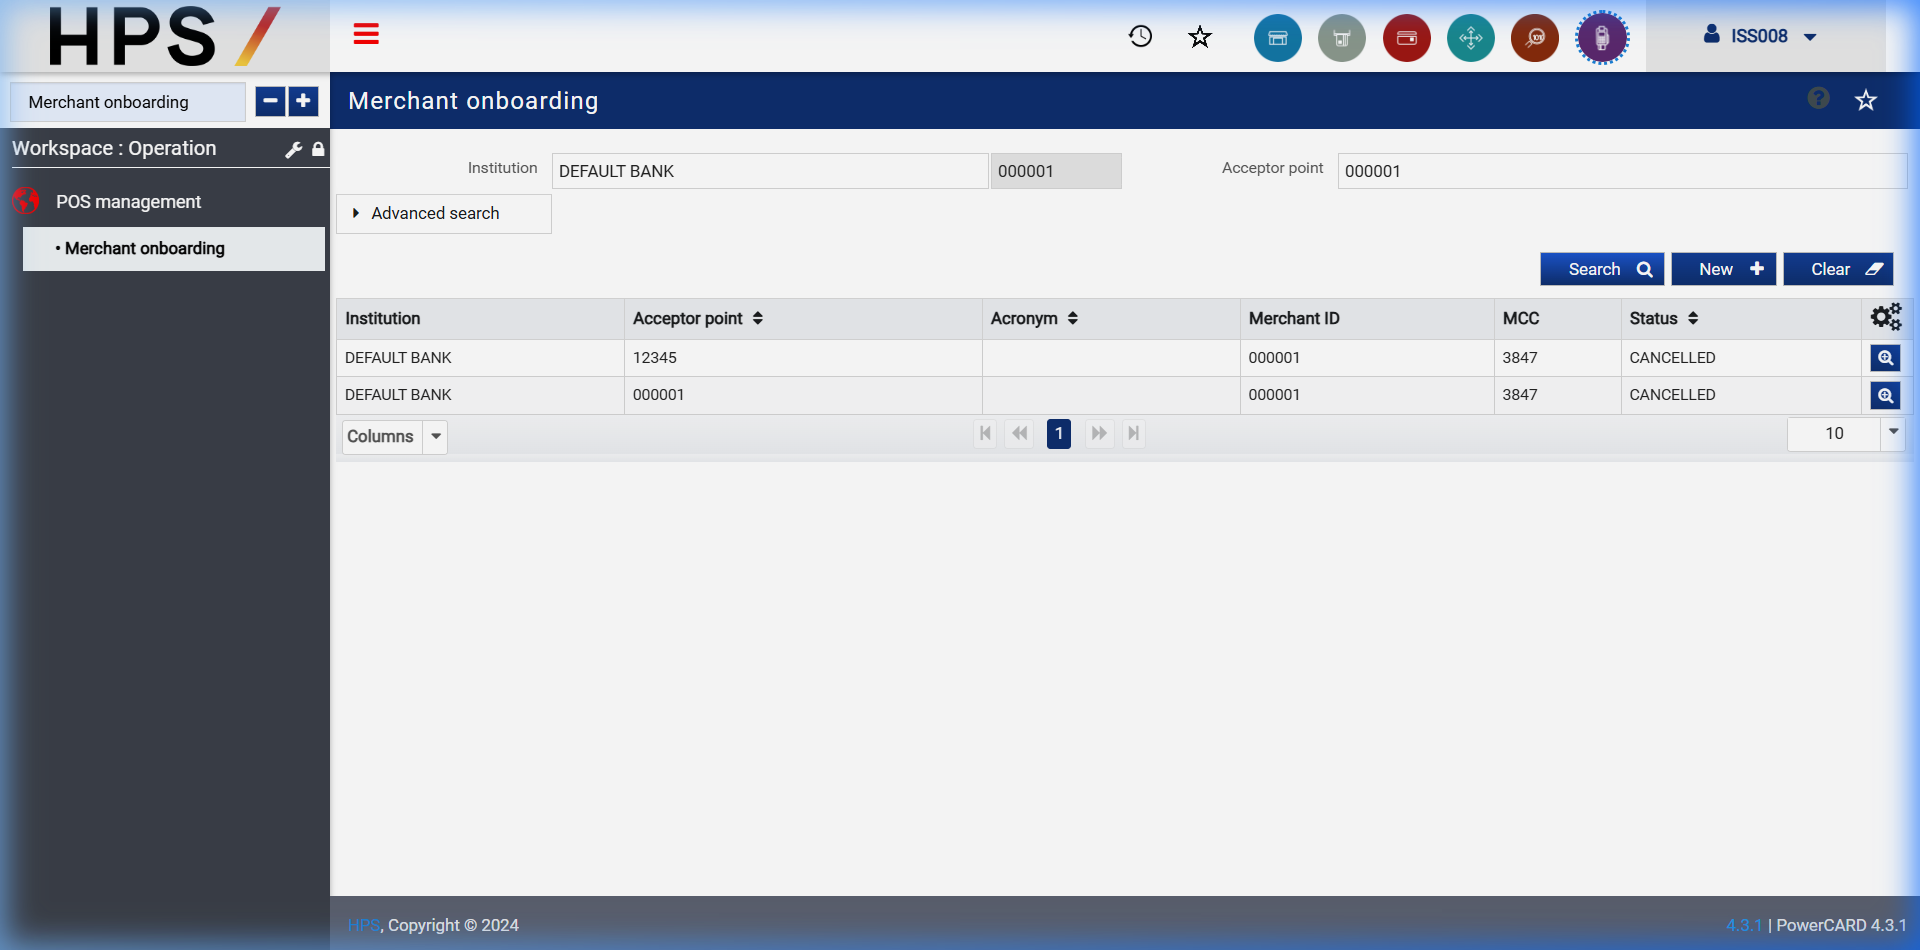
\includegraphics[width=0.8\textwidth]{step16_result.png}
    \caption{Résultat final de la recherche --- Le marchand est trouvé dans la liste}
\end{figure}


% ── Journal des Tickets Jira ──
\newpage
\subsection{Journal Officiel des Tickets Jira}

\subsubsection{[BF-911] Données non conservées dans le champ Ville}

\begin{tcolorbox}[colback=white, colframe=primary, title=\textbf{Ticket Jira : BF-911}, fonttitle=\bfseries]
\textbf{Environnement :} \texttt{bo\_fe\_develop} | \textbf{Cluster :} \texttt{Andromed}

\textbf{Étapes :}
\begin{enumerate}[leftmargin=1.5em]
    \item Écran d'intégration du marchand → Nouveau → Remplir tous les champs → Enregistrer.
    \item Retour → Rechercher l'enregistrement → Double-cliquer → Aller à Localisation.
\end{enumerate}

\bugtable{Le champ \textbf{Ville} ne doit pas être vide.}
         {Le champ \textbf{Ville} est vide.}
\end{tcolorbox}

\subsubsection{[BF-912] Indicateur d'onglet incorrect}

\begin{tcolorbox}[colback=white, colframe=primary, title=\textbf{Ticket Jira : BF-912}, fonttitle=\bfseries]
\textbf{Environnement :} \texttt{bo-fe-develop} | \textbf{Cluster :} \texttt{Andromed}

\bugtable{L'onglet doit devenir rouge si des champs obligatoires sont manquants.}
         {L'onglet reste vert.}
\end{tcolorbox}

\twoimages{user_img4.png}{Résultat Attendu (L'onglet devient ROUGE)}
          {user_img3.png}{Résultat Obtenu (L'onglet reste VERT)}

\subsubsection{[BF-921] Enregistrement échoue --- Erreur critique}

\begin{tcolorbox}[colback=white, colframe=primary, title=\textbf{Ticket Jira : BF-921}, fonttitle=\bfseries]
\textbf{Environnement :} \texttt{bo-fe-develop} | \textbf{Cluster :} \texttt{Andromed}

\bugtable{Le mapping doit être enregistré avec succès.}
         {Erreur 500 : « Create Problem. Objects creation could not be performed ».}
\end{tcolorbox}

\begin{figure}[H]
    \centering
    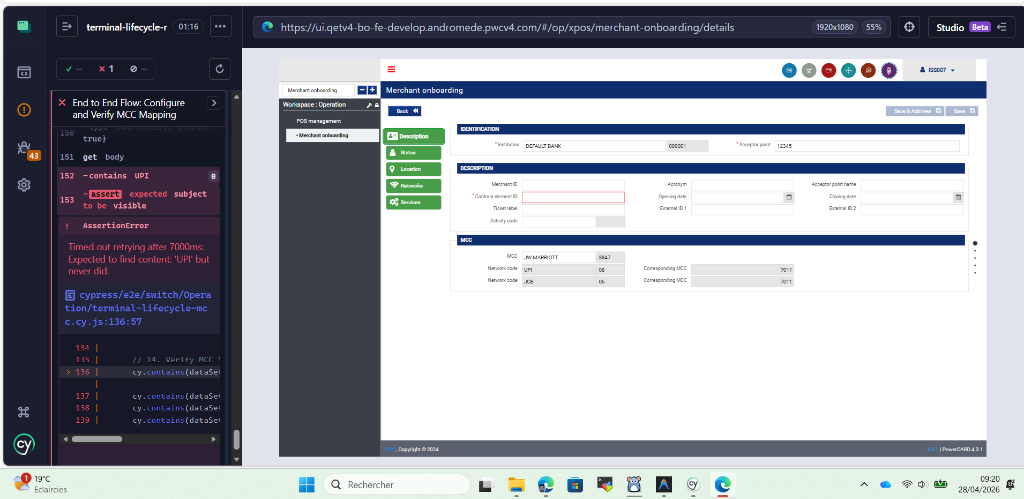
\includegraphics[width=0.8\textwidth]{failure.png}
    \caption{Preuve : Fenêtre d'erreur rouge lors de l'enregistrement}
\end{figure}


% ── Résumé des Bugs ──
\subsection{Résumé des Bugs}

\begin{center}
\renewcommand{\arraystretch}{1.4}
\begin{tabularx}{\textwidth}{|c|c|c|R|R|}
\hline
\rowcolor{primary!15}\textbf{\#} & \textbf{Type} & \textbf{Clé Jira} & \textbf{Titre} & \textbf{Description} \\
\hline
1 & \textcolor{danger}{\textbf{Défaut}} & BF-911 & Données non conservées dans le champ ``Ville'' & Le champ ville s'affiche vide après confirmation et réouverture. \\
\hline
2 & \textcolor{danger}{\textbf{Défaut}} & BF-912 & L'indicateur d'onglet reste vert & L'onglet reste VERT même avec des champs obligatoires en erreur. \\
\hline
3 & \textcolor{warning}{\textbf{Défaut/Processus}} & BF-916 & Validation du tableau & Lignes infinies, validation longueur manquante, infobulles absentes. \\
\hline
4 & \textcolor{danger}{\textbf{Défaut Critique}} & BF-921 & Enregistrement échoue & Erreur 500 lors de l'enregistrement de l'ensemble des mappings. \\
\hline
\end{tabularx}
\end{center}


\vspace{10pt}
\textbf{Conclusion}

En conclusion, ce chapitre a concrétisé l'aboutissement de mon projet de fin d'études en démontrant la viabilité technique des solutions proposées. L'automatisation réussie des flux fonctionnels PowerCARD garantit une détection rapide et fiable des régressions. La démonstration pratique du flux MOTO a illustré de manière concrète comment le Dashboard permet à un testeur de générer, exporter et exécuter un test complet en quelques minutes, sans écrire une seule ligne de code. Parallèlement, le rapport QA a mis en évidence la capacité de l'outil à identifier des défauts critiques dans l'application. Le dernier chapitre s'attachera à évaluer le bilan de ce projet et ses apports globaux.


% ── Chapitre V: Les apports du projet ──
% ══════════════════════════════════════════════════════════════════
% CHAPITRE V — Les apports du projet
% ══════════════════════════════════════════════════════════════════
\newpage
\chapter{Les apports du projet}
\vspace{1cm}
\minitoc
\newpage

\textbf{Introduction}

L'évaluation d'un stage de fin d'études ne se limite pas à la simple énumération des tâches techniques accomplies ; elle réside également dans l'analyse de la valeur ajoutée apportée à l'entreprise et des bénéfices tirés par le stagiaire. Ce cinquième et dernier chapitre propose une réflexion rétrospective sur l'ensemble de l'expérience vécue au sein d'HPS. Nous aborderons d'abord l'impact du projet d'automatisation sur l'efficacité opérationnelle des équipes de test, avant de dresser un bilan des compétences techniques, méthodologiques et comportementales acquises tout au long de cette période d'immersion professionnelle.
\vspace{10pt}

Durant les six mois de stage que j'ai passé à la société HPS, j'ai pu contribuer efficacement au processus de tests dans un des produits PowerCARD. Les tests que j'ai menés avec mon équipe ont permis de vérifier le fonctionnement du produit.

L'équipe au sein de laquelle j'ai travaillé a l'expérience et le savoir-faire nécessaires pour produire la meilleure qualité possible, garantir que le produit ne présent pas de bogues ou d'erreurs, et par conséquent, satisfaire les besoins de la clientèle.

Grâce aux preuves tangibles des tests, l'entreprise a pu collecter des domaines pour les améliorations possibles nécessaires pour le développement de son produit. Le produit que doit livrer au client permettra sûrement à la société de se faire une image de marque, chose indispensable pour son développement et sa croissance.

\section{Bénéfices du Dashboard pour l'entreprise}

Le développement du QA Cypress Generator Dashboard a apporté des bénéfices concrets et mesurables à l'équipe QA d'HPS :

\begin{table}[H]
\centering
\caption{Comparaison avant/après l'automatisation}
\renewcommand{\arraystretch}{1.4}
\begin{tabularx}{\textwidth}{l X X}
\toprule
\textbf{Critère} & \textbf{Avant (Manuel)} & \textbf{Après (Dashboard)} \\
\midrule
\rowcolor{primary!5} Temps de création d'un test & 30--60 min (écriture code) & 3--5 min (formulaire) \\
Compétences requises & JavaScript avancé, Cypress API & Aucune compétence code \\
\rowcolor{primary!5} Risque d'erreurs & Élevé (typos sélecteurs) & Faible (auto-génération) \\
Couverture des écrans & Limitée (écrans connus) & 32 écrans catalogués \\
\rowcolor{primary!5} Données de test & Manuelles (copier/coller) & Auto-Fill via API Connect \\
Exécution des tests & Terminal séparé & Intégrée dans le Dashboard \\
\rowcolor{primary!5} Rapport de résultats & Logs bruts Cypress & Rapport visuel temps réel \\
\bottomrule
\end{tabularx}
\end{table}

\subsection{Gains quantitatifs}

\begin{itemize}[leftmargin=*]
\item \textbf{Réduction du temps de 85\%} : La génération automatique des scripts réduit le temps de création d'un scénario de test de 45 minutes en moyenne à moins de 5 minutes.
\item \textbf{32 écrans catalogués automatiquement} : Le scanner de catalogue détecte et indexe les specs existantes sans intervention manuelle.
\item \textbf{5 endpoints API} : L'architecture microservices expose 5 endpoints REST/SSE couvrant l'ensemble du cycle de vie du test.
\item \textbf{Zéro ligne de code requise} : Les testeurs fonctionnels peuvent générer des tests complets via l'interface graphique.
\end{itemize}

\subsection{Gains qualitatifs}

\begin{itemize}[leftmargin=*]
\item \textbf{Démocratisation de l'automatisation} : Les testeurs non-développeurs peuvent désormais participer à l'effort d'automatisation.
\item \textbf{Standardisation des scripts} : Tous les tests générés suivent la même structure et les mêmes conventions.
\item \textbf{Traçabilité} : Chaque test généré est lié à un écran PowerCARD identifié dans le catalogue.
\item \textbf{Intégrité des données} : L'auto-remplissage via l'API Connect garantit l'utilisation de données de test valides.
\end{itemize}

\section{Apport de l'Intelligence Artificielle}

L'intégration de Mistral AI dans le Dashboard a ouvert de nouvelles perspectives :

\begin{itemize}[leftmargin=*]
\item \textbf{Découverte automatique d'écrans} : Le crawler Cypress parcourt les modules PowerCARD et extrait les schémas d'écrans bruts. Mistral AI analyse ces schémas pour les classifier (module, workspace), générer des labels lisibles, et suggérer les meilleures stratégies de sélection pour chaque champ.
\item \textbf{Génération de tests par IA} : Le service \texttt{generator-service} utilise Mistral pour produire des scripts Cypress complets à partir de descriptions fonctionnelles.
\item \textbf{Enrichissement du catalogue} : L'IA comble les lacunes des templates manuels en inférant automatiquement les types de champs et les valeurs de test suggérées.
\end{itemize}

\section{Apport de n8n}

L'intégration de n8n comme outil d'orchestration a permis :

\begin{itemize}[leftmargin=*]
\item \textbf{Automatisation de la préparation des données} : Les workflows n8n récupèrent automatiquement les cartes de test via l'API Connect et les stockent dans la base SQLite.
\item \textbf{Archivage automatique} : Les résultats de tests sont archivés dans la base de données pour suivi historique.
\item \textbf{Orchestration sans code} : Les testeurs peuvent créer des workflows complexes de préparation de données via l'interface visuelle de n8n.
\end{itemize}

\section{Apports personnels}

Grace à ce stage, j'ai pu réaliser, au sein de mon équipe, différentes tâches dans le processus de test. Ceci m'a permis d'améliorer davantage mes compétences techniques, professionnelles et humaines.

Ce projet, très riches en enseignements, m'a confirmé l'importance du test dans les projets de développement logiciel. Ce qui m'a incité à persévérer et s'impliquer davantage dans ce métier.

\subsection{En termes de compétences techniques}

\begin{itemize}[leftmargin=*]
\item Maîtrise du framework Cypress pour l'automatisation de tests E2E,
\item Développement full-stack avec React, Node.js et Vite,
\item Architecture microservices et containerisation Docker,
\item Intégration d'APIs d'intelligence artificielle (Mistral AI),
\item Mise en place de workflows d'automatisation avec n8n,
\item Gestion de bases de données SQLite,
\item Utilisation de Server-Sent Events (SSE) pour le streaming temps réel.
\end{itemize}

\subsection{En termes de travail en équipe}

Le projet m'a permis de développer diverses capacités, entre autres :
\begin{itemize}[leftmargin=*]
\item La communication entre équipes ou membres d'une même équipe, en temps réel,
\item La coordination avec les autres équipes pour le lancement des scripts d'automatisation,
\item L'adaptation aux méthodes de travail des parties prenantes du projet.
\end{itemize}

\subsection{En termes de travail sur le terrain}

Ceci, qui est nouveau pour moi, m'a apporté :
\begin{itemize}[leftmargin=*]
\item Une certaine maturité quasi-immédiate, qui m'a permis de comprendre comment cibler les problèmes prioritaires,
\item L'aptitude à améliorer mon autonomie vis-à-vis de la prise de décision,
\item L'importance de la rigueur, du respect des engagements, des délais.
\end{itemize}

\vspace{10pt}
\textbf{Conclusion}

L'ensemble de ces apports témoigne de l'impact positif de cette expérience sur mon profil d'ingénieur. Ce projet m'a permis non seulement de valider mes compétences techniques, mais également d'acquérir une posture professionnelle solide et de comprendre les enjeux réels de la qualité logicielle en entreprise. L'intégration de technologies de pointe comme l'intelligence artificielle et l'orchestration de workflows positionne ce projet comme une contribution significative à la modernisation des processus QA chez HPS.


% ── Conclusion Générale et Perspectives ──
% ══════════════════════════════════════════════════════════════════
% CONCLUSION GÉNÉRALE ET PERSPECTIVES
% ══════════════════════════════════════════════════════════════════
\newpage
\chapter*{Conclusion Générale et Perspectives}
\addcontentsline{toc}{chapter}{Conclusion Générale et Perspectives}

Ce stage de projet de fin d'études pendant 6 mois était intéressant et bénéfique pour moi, car j'ai pu mettre en pratique les connaissances théoriques et techniques acquises à l'université EMSI, en travaillant sur un projet concret et en contribuant activement à l'amélioration d'un système logiciel fourni par la société d'accueil.

Je suis à la fois fier et satisfait de mon stage au sein de la Société HPS Group. Car, ce stage m'a permis d'apprécier de plus près la vie professionnelle au sein d'une société, travailler en parfaite harmonie au sein d'une équipe et découvrir dans le détail comment gérer et réaliser un projet du début jusqu'à la fin.

Au sein d'HPS, j'ai pu m'ouvrir sur le domaine de test qui m'a permis de travailler sur des sujets qui partagent le même contexte. Ce projet m'a permis d'approfondir mes connaissances dans le métier de test avec une formation sur l'ISTQB et les sujets d'automatisation.

J'ai beaucoup apprécié les missions qui m'ont été confiés. Car, d'abord, elles s'inscrivent dans le cadre de mon projet personnel, ensuite elles m'ont permis de découvrir les étapes du processus de test, de l'expression des besoins jusqu'à la fin.

Tout au long de ce stage, j'avais un suivi et un encadrement de qualité, trois réunions par semaine avec l'équipe de test pour suivre mon avancement, et pour faire le point sur les points de blocage et tâches à venir.

Les difficultés que j'ai vécu durant mon stage sont principalement liées à l'incomplétude des cahiers de spécification et l'environnement technique de travail. Travailler sur cette difficulté m'a donné la possibilité de communiquer avec plusieurs personnes et de ne pas rester renfermée sur moi-même, et donc de s'intégrer plus facilement au sein de l'entreprise.

Pour conclure, ce stage de fin d'études a constitué une opportunité exceptionnelle d'évoluer au sein d'un environnement professionnel exigeant, centré sur l'innovation et la qualité des systèmes de paiement. La réalisation du Cypress Generator Dashboard et l'automatisation des tests fonctionnels ont répondu concrètement à un besoin d'optimisation des processus QA. L'intégration de l'intelligence artificielle (Mistral AI) pour la découverte automatique d'écrans et la génération de tests, combinée à l'orchestration des workflows via n8n, positionne cette solution comme un outil de nouvelle génération dans le domaine de l'assurance qualité logicielle.

Les connaissances acquises en ingénierie logicielle, couplées à une immersion dans les méthodologies de travail collaboratives, consolident ma formation d'ingénieur. Ce projet confirme l'importance stratégique de l'automatisation dans le cycle de vie logiciel moderne, ouvrant des perspectives prometteuses pour ma carrière future dans le domaine de la qualité et du développement logiciel.

\textbf{Perspectives d'amélioration :}
\begin{itemize}[leftmargin=*]
\item Intégration d'un modèle d'IA local (type LLM auto-hébergé) pour éliminer la dépendance aux API externes,
\item Extension du crawling AI à l'ensemble des modules PowerCARD pour couvrir 100\% des écrans,
\item Mise en place d'un pipeline CI/CD complet intégrant le Dashboard comme étape de génération automatique des tests de régression,
\item Développement d'un mode batch pour l'exécution parallèle de multiples scénarios de test,
\item Ajout d'un système de reporting avancé avec historique des exécutions et tendances de qualité.
\end{itemize}


% ── Références ──
% ══════════════════════════════════════════════════════════════════
% BIBLIOGRAPHIE & WEBOGRAPHIE
% ══════════════════════════════════════════════════════════════════
\newpage
\chapter*{Références}
\addcontentsline{toc}{chapter}{Références}

\section*{Bibliographie}
\begin{enumerate}
\item HPS, Documentation interne PowerCARD, 2022
\item ISTQB, \textit{Certified Tester Foundation Level Syllabus}, Version 4.0, 2023
\item Rex Black, Dorothy Graham, Erik van Veenendaal, \textit{Foundations of Software Testing: ISTQB Certification}, Cengage Learning, 2012
\end{enumerate}

\section*{Webographie}
\begin{enumerate}
\item {[En ligne]}: HPS Worldwide - Feel good about payments --- \url{https://hps-worldwide.com}
\item {[En ligne]}: HPS eAcademy: Se connecter sur le site --- \url{https://hps-eacademy.com}
\item {[En ligne]}: Refertest, votre solution de management de tests --- \url{https://referty.com}
\item {[En ligne]}: HPS Fluid Topics Documentation --- \url{https://hps.fluidtopics.net/}
\item {[En ligne]}: Cypress Documentation officielle --- \url{https://docs.cypress.io}
\item {[En ligne]}: React Documentation --- \url{https://react.dev}
\item {[En ligne]}: Vite --- Next Generation Frontend Tooling --- \url{https://vitejs.dev}
\item {[En ligne]}: Node.js Documentation --- \url{https://nodejs.org/docs}
\item {[En ligne]}: Mistral AI --- Documentation API --- \url{https://docs.mistral.ai}
\item {[En ligne]}: n8n --- Workflow Automation Tool --- \url{https://docs.n8n.io}
\item {[En ligne]}: Monaco Editor --- \url{https://microsoft.github.io/monaco-editor}
\item {[En ligne]}: Docker Documentation --- \url{https://docs.docker.com}
\item {[En ligne]}: SQLite Documentation --- \url{https://www.sqlite.org/docs.html}
\end{enumerate}


\end{document}